\documentclass[UTF8, fontset=none]{ctexart}
\usepackage{fontspec}
% \usepackage[utf8]{inputenc}
\usepackage{authblk} % for author affiliations
\usepackage{hyperref}
\usepackage{graphicx}
\usepackage{amsmath}
\usepackage{amssymb}
\usepackage{pgfplotstable}
\usepackage{booktabs} % for table formatting
\usepackage{caption}
\usepackage{subcaption}
\usepackage{enumitem}
\usepackage{geometry}
\usepackage{float}
\usepackage{pgffor}
\usepackage{longtable}
\setCJKmainfont{Noto Serif CJK TC Black}
% \geometry{margin=1cm}
\geometry{a4paper, margin=2.5cm}




\title{Visual Prompt Engineering for ChatGPT-4o: A Low-Resource Fine-Tuning Approach}

\author[1]{You-Jia Syu}
\author[1]{Sheng-An Yang}
\affil[1]{Independent Researcher}

\date{\today}

\begin{document}

\maketitle

\begin{abstract}
在在本研究中,我們探索了視覺語言模型(VLMs)於鋼材識別任務中的應用潛力。任務目標為:輸入包含鋼材形狀結構與尺寸標註的圖像,模型需自動判斷該鋼材對應的類型(如 A001、A002 等)與邊長資訊。圖像中雖包含數字與結構線條,卻未直接標示類別代碼,模型需藉由圖形幾何配置與數值關係進行推理。我們在不擴充訓練資料的前提下,提出數種輸入設計與提示策略,有效提升模型辨識準確率。實驗結果顯示,即便在低資源條件下,透過適當的輸入結構與視覺提示設計,VLM 仍能在實務場景中展現良好的識別效果。
\end{abstract}

\section{前言}
近年來,隨著 ChatGPT \cite{openai2024gpt4o}等大型語言模型(LLMs)技術迅速發展,其跨領域的應用潛力也日益受到重視。許多企業與研究單位開始思考,是否能藉由這類通用型人工智慧,解決實際產業場域中的自動化挑戰。本研究便是在這樣的背景下展開:我們嘗試將 ChatGPT 應用於鋼鐵產業中的圖形識別任務,以協助業主進行生產流程的智慧化轉型。

我們的合作對象為一家鋼材加工廠商。過往,該公司需仰賴具備專業背景的人工操作人員,手動將鋼材圖面資訊(包含幾何結構與尺寸標註)轉錄至其內部的 ERP 系統中。此流程不僅耗時費工,也容易因人工輸入失誤導致後續錯誤。我們希望透過 AI 模型導入,能將該流程自動化,以降低成本並提升資料正確性。

然而,自動化流程中最具挑戰性的一步,便是「圖形識別」。這些鋼材圖像通常僅包含幾何線條與數字標註,未附上明確的類別代碼,因此模型需具備一定程度的空間理解與邏輯推理能力。為此,我們選擇探索使用 ChatGPT 進行圖像分析的可能性,並透過不同的提示設計與輸入編排方式,嘗試引導其正確解讀圖像資訊。

本研究記錄了我們在這一過程中的實驗設計與關鍵觀察,並初步驗證 ChatGPT 在特定條件下確實具備一定的圖形理解能力,對未來跨模態的產業應用提供了有價值的參考。
\section{實驗設計}

為驗證大型語言模型於鋼材圖形識別任務中的應用效能,我們設計了一系列基於 ChatGPT-4o 的微調實驗。本節將說明資料來源與處理方式,以及實際訓練時所採用的模型與參數設定。
\subsection{模型能力目標}
在本任務中,我們預期模型能夠具備以下能力:
\begin{itemize}
  \item 根據幾何結構與尺寸標註,推論對應的鋼材類別
  \item 識別手寫與印刷混合的文字標註
  \item 處理圖像的旋轉與翻轉變化,保持識別準確度
  \item 解讀圖形中未明確標示但可推論出的邊長資訊
\end{itemize}

\begin{figure}[H]
    \centering
    \includegraphics[width=0.9\textwidth]{figure/Model_Capability_Objectives.png}
    \caption{Model Capability Objectives}
    \label{fig:model-capability}
\end{figure}
\subsection{資料來源與建構方式}

本研究所使用的鋼材圖面資料,原始來源為合作廠商所提供的部分真實圖像。這些圖面採工程繪圖格式,包含鋼材的幾何結構與尺寸標註,內容接近實務中輸入 ERP 系統所需的格式。然而,因涉及商業機密,原始圖像無法直接用於模型訓練或公開發表。

為兼顧資料保密與研究需求,我們參考原始圖面的風格與構成邏輯,人為合成一批具代表性的鋼材圖面資料集。該資料模擬實際場景中的圖形樣式,包括常見的 L 型、U 型、方形鋼材輪廓,以及多種尺寸標示方式,作為模型訓練與測試使用。

\paragraph{鋼材種類與風格}
\begin{itemize}
  \item \textbf{鋼材種類}:共構建 6 種鋼材類別,分別為 C105、C106、C413、C445、C505、C603。
  \item \textbf{書寫風格}:每種鋼材各包含三種變異風格:
    \begin{enumerate}
      \item 全印刷(Printed Only)
      \item 圖形印刷+手寫尺寸(Mixed)
      \item 全手寫(Handwritten Only)
    \end{enumerate}
\end{itemize}

\paragraph{資料生成與處理方式}
\begin{itemize}
  \item 印刷部分以小畫家繪製(線條粗細為 5pt,字型使用 \texttt{Calibri}),經印表機列印輸出。
  \item 手寫部分由六位同事獨立填入隨機數字(1--100),確保筆跡與內容具備多樣性與獨立性。
  \item 列印後之圖像以掃描方式數位化,再依圖形區域進行裁切,取得標準化樣本。
\end{itemize}

\paragraph{資料擴增策略}
每張圖像樣本進行以下變換操作,以提升模型的泛化能力:
\begin{itemize}
  \item 旋轉四個角度:$0^\circ$, $90^\circ$, $180^\circ$, $270^\circ$
  \item 搭配水平翻轉(flip)後再旋轉,共計 8 種資料版本
\end{itemize}
此外,每張圖像皆搭配一組人工標註的標籤(label),作為模型訓練與評估之依據。由於翻轉搭配旋轉的變換與原始圖像在幾何結構上等價,因此其標註結果應保持一致,確保模型學習專注於圖形內容而非圖像位置。

\paragraph{資料命名與屬性欄位}
每張圖像資料皆對應一組組合屬性,以利於後續分類與實驗設計。命名結構由以下欄位組成:

\begin{itemize}
  \item \texttt{classes}:鋼材類別,共 6 種:\texttt{C105}、\texttt{C106}、\texttt{C413}、\texttt{C445}、\texttt{C505}、\texttt{C603}
  \item \texttt{hand\_types}:書寫風格類型,共 3 種:\texttt{printed\_only}、\texttt{mixed\_print\_hand}、\texttt{handwritten\_only}
  \item \texttt{flip}:是否經水平翻轉,包含 \texttt{flip} 與 \texttt{no\_flip}
  \item \texttt{rot}:旋轉角度,包含 \texttt{rot0}、\texttt{rot1}、\texttt{rot2}、\texttt{rot3}
  \item \texttt{groups}:資料分組,分為 \texttt{train} 與 \texttt{test}
\end{itemize}

每張圖像都會對應一組標籤(tag),以管線符號(\texttt{|})串接各屬性資訊。例如:\texttt{C105\textbar{}handwritten\_only\textbar{}flip\textbar{}rot1\textbar{}test},表示該圖像屬於 C105 類型、手寫風格,並經翻轉與 $90^\circ$ 旋轉處理。最後的分組標籤(如 \texttt{train} 或 \texttt{test})視實驗需求而定,並非固定劃分。


\paragraph{資料集規模}
\begin{itemize}
  \item 每種類鋼材原始樣本數:24 張
  \item 擴增後每類:$24 \times 8 = 192$ 張
  \item 資料總量:$6 \times 192 = \mathbf{1,152}$ 張圖像
\end{itemize}

為提升主文清晰度,完整圖像範例與表格展示另收錄於附錄中。

\subsection{模型設定與訓練參數}

考量目前僅有 GPT-4o (版本日期:2024-08-06) 支援視覺語言模型(VLM)的微調功能,本研究即採用該版本進行後續實驗。模型訓練採用監督式學習(Supervised Fine-tuning)方式進行,相關訓練參數設定如下:

\begin{itemize}[leftmargin=2em]
  \item \textbf{模型版本}:GPT-4o (gpt-4o-2024-08-06)
  \item \textbf{訓練方法}:監督式微調(Supervised Fine-tuning)
  \item \textbf{訓練輪數(Epochs)}:3
  \item \textbf{每批樣本數(Batch size)}:4
  \item \textbf{學習率倍率(LR multiplier)}:2
  \item \textbf{隨機種子(Seed)}:3407
\end{itemize}



以上設定在 OpenAI 提供之微調平台上完成,並針對我們建構的資料集進行多輪訓練與評估。
\paragraph{評分指標定義}
為衡量模型輸出的完整性與正確性,我們設計四項遞進式指標;每通過一道「關卡」才會進入下一層評估,最終若全部滿足,則記為 \texttt{all\_correct}=1。

\begin{enumerate}[label=\textbf{\arabic*.}]
  \item \textbf{\texttt{json\_correct}}  
        模型回傳內容必須能被成功解析為合法 \textsc{JSON};若解析失敗,直接計為 0,並跳過後續評分。
        
  \item \textbf{\texttt{structure\_correct}}  
        在 \texttt{json\_correct}=1 的前提下,檢查關鍵欄位是否齊備且符合資料格式規範。  
        非必要或多餘欄位不影響此項評分。
        
  \item \textbf{\texttt{type\_correct} 與 \texttt{edge\_correct}}(獨立計算)  
        \begin{enumerate}[leftmargin=*, label*=\arabic*.]
            \item 若鋼材\emph{類型}預測正確,則 \texttt{type\_correct}=1。  
            \item 若鋼材\emph{各邊長}皆預測正確,則 \texttt{edge\_correct}=1。
        \end{enumerate}

  \item \textbf{\texttt{all\_correct}}  
        當 \texttt{json\_correct}、\texttt{structure\_correct}、\texttt{type\_correct}、\texttt{edge\_correct} 均為 1 時,\
        記為完全正確 (\texttt{all\_correct}=1)。
\end{enumerate}
\begin{figure}[H]
    \centering
    \includegraphics[width=0.9\textwidth]{figure/correctness_evaluation_flow.png}
    \caption{Correctness Evaluation Flow}
    \label{fig:correctness-flow}
\end{figure}

\section{實驗}
我們一共進行了四次的模型訓練(model0,model1,model2,model3),其中前三次成功了,最後一次不算成功

\subsection{實驗0:樸素的嘗試}
非常簡單的嘗試,就是模型接收圖片,直接吐出JSON,結果非常的糟糕,在train的正確是22(30.56\%),test是70 (6.48\%)

\subsection*{錯誤案例分析}
分析
\subsection{實驗1:加入 full\_image 改善}
train的正確是 32 (44.44\%),test是121 (11.20\%)
\subsection{實驗2:加入prefix prompt 穩定json輸出}
如圖 \ref{fig:model0:lossacc} 所示,Model 0 的 loss 在第二 epoch 後穩定下降。
json\_correct是1152 (100.00\%),相較於實驗1 1067 (92.62\%)
由於json被正確了的解析, train正確率65 (90.28\%),test正確率212 (19.63\%)
\subsection{將旋轉的圖片也加進去train資料}
這邊有點失敗
train正確率234 (81.25\%),test的正確率157 (18.17\%)
\section{Conclusion and Future Work}
We demonstrate that even with limited data, structured and iterative refinement---starting with simple prompt-based training and gradually introducing data- and process-driven enhancements---can lead to meaningful improvements in VLM performance. Future work will explore automatic error pattern mining and dynamic prompt tuning.

\bibliographystyle{plain}
\bibliography{references}
  

\appendix
\section{資料準備}
\subsection{空的圖片}
\begin{figure}[H]
  \centering

  \begin{subfigure}[b]{0.3\textwidth}
    \fbox{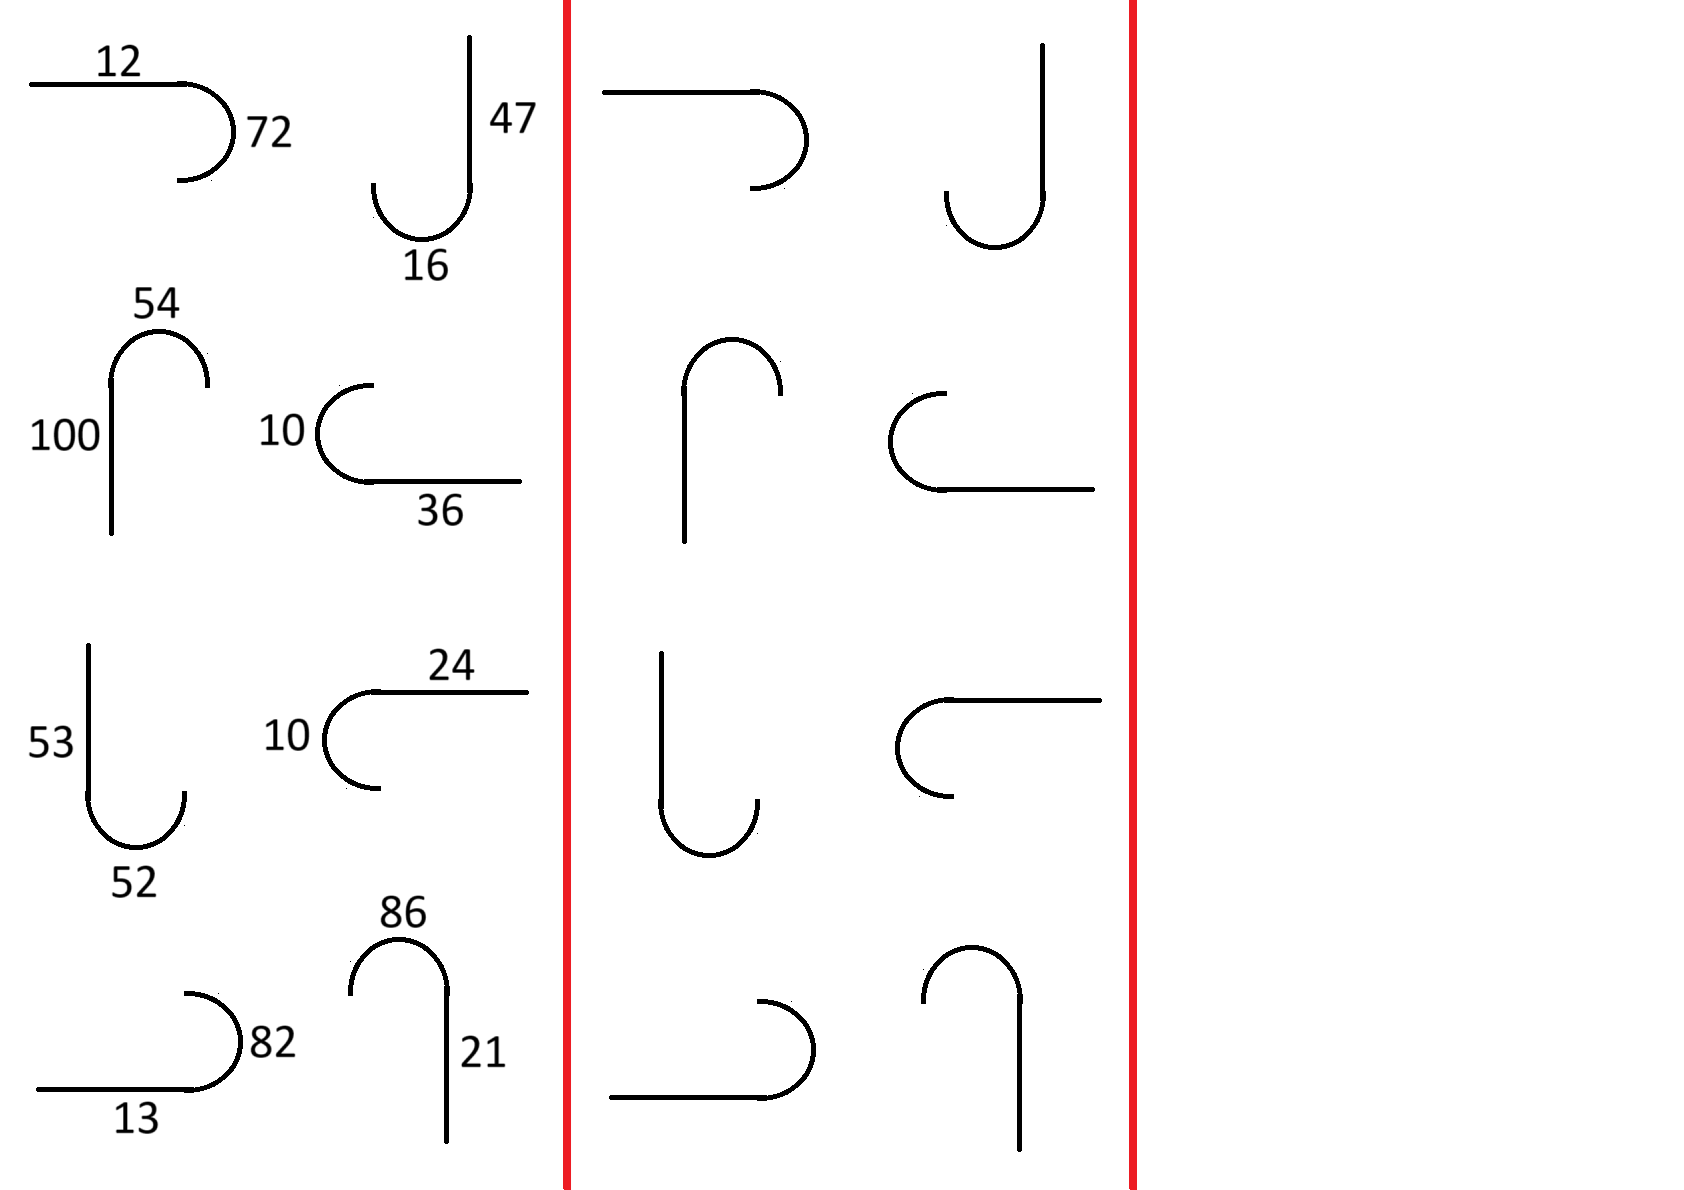
\includegraphics[width=\textwidth]{./figure/C105.png}}
    \caption{C105}
    \label{fig:C105:origin}
  \end{subfigure}
  \hfill
  \begin{subfigure}[b]{0.3\textwidth}
    \fbox{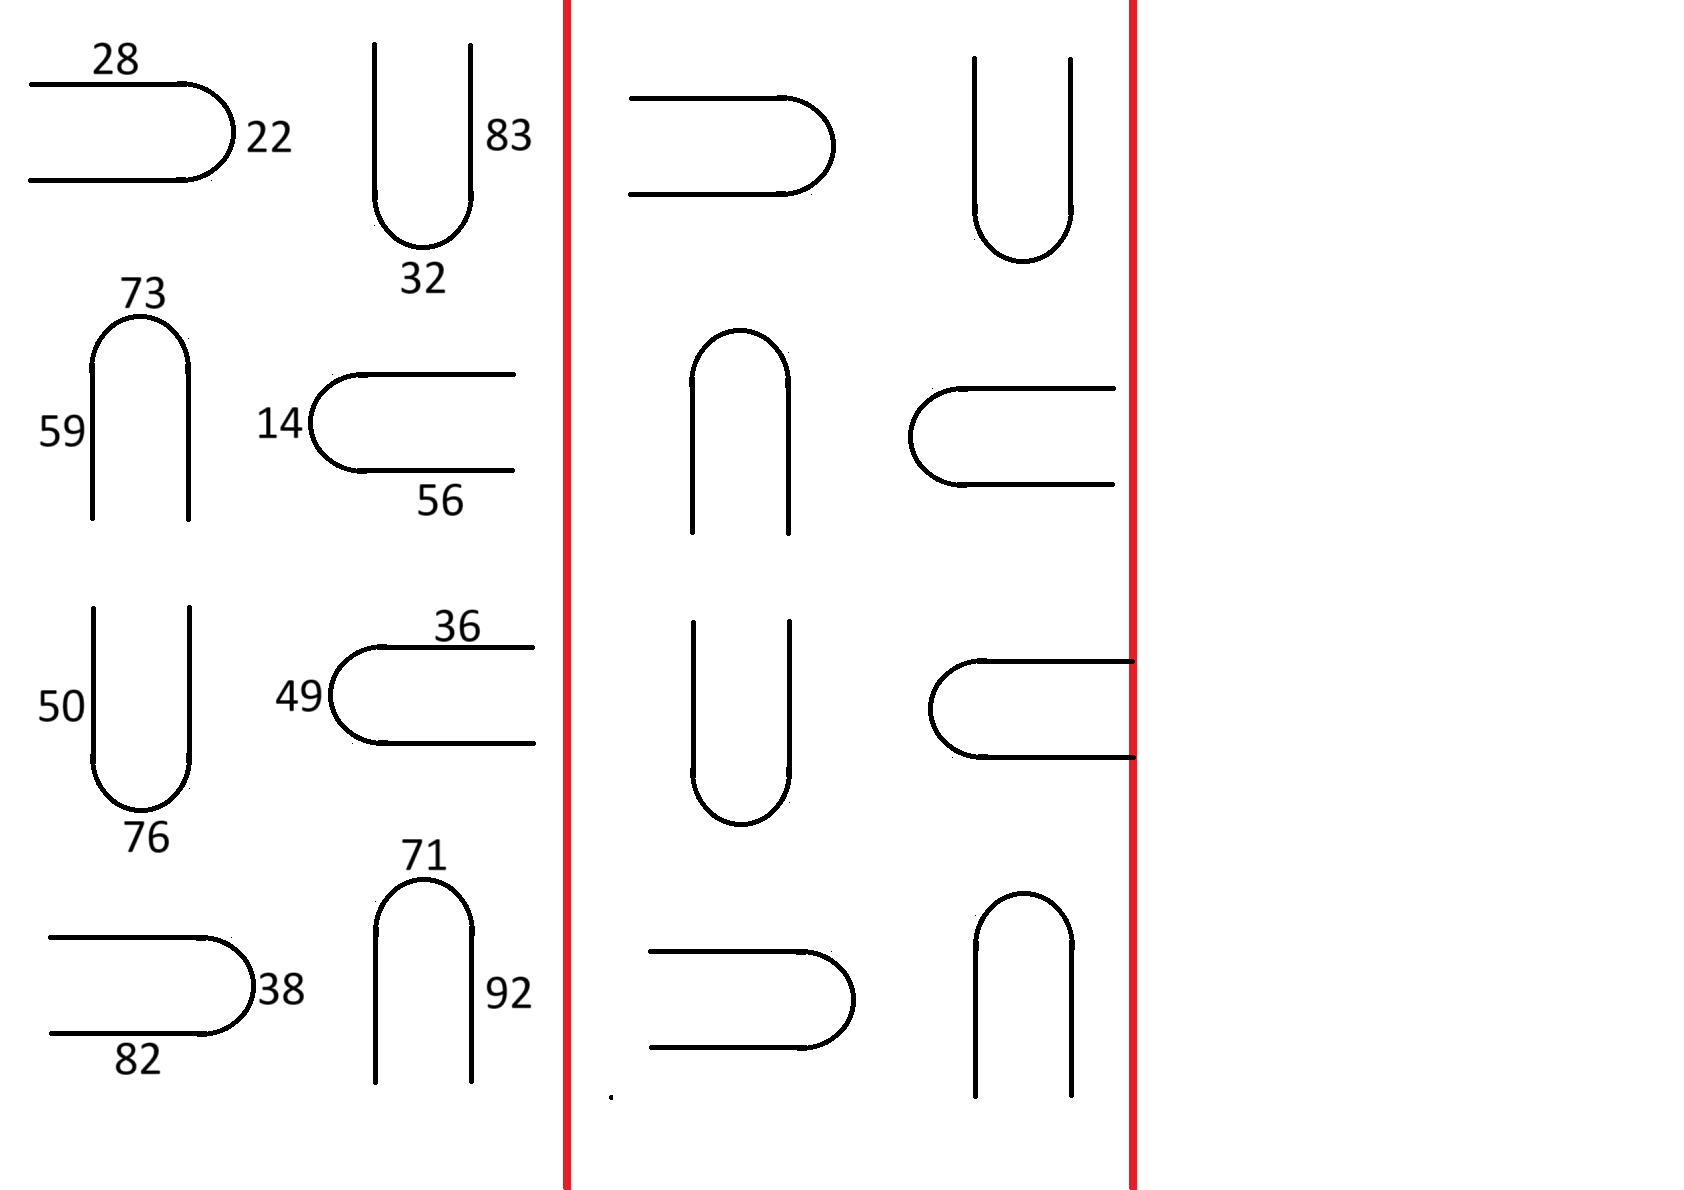
\includegraphics[width=\textwidth]{./figure/C106.png}}
    \caption{C106}
    \label{fig:C106:origin}
  \end{subfigure}
  \hfill
  \begin{subfigure}[b]{0.3\textwidth}
    \fbox{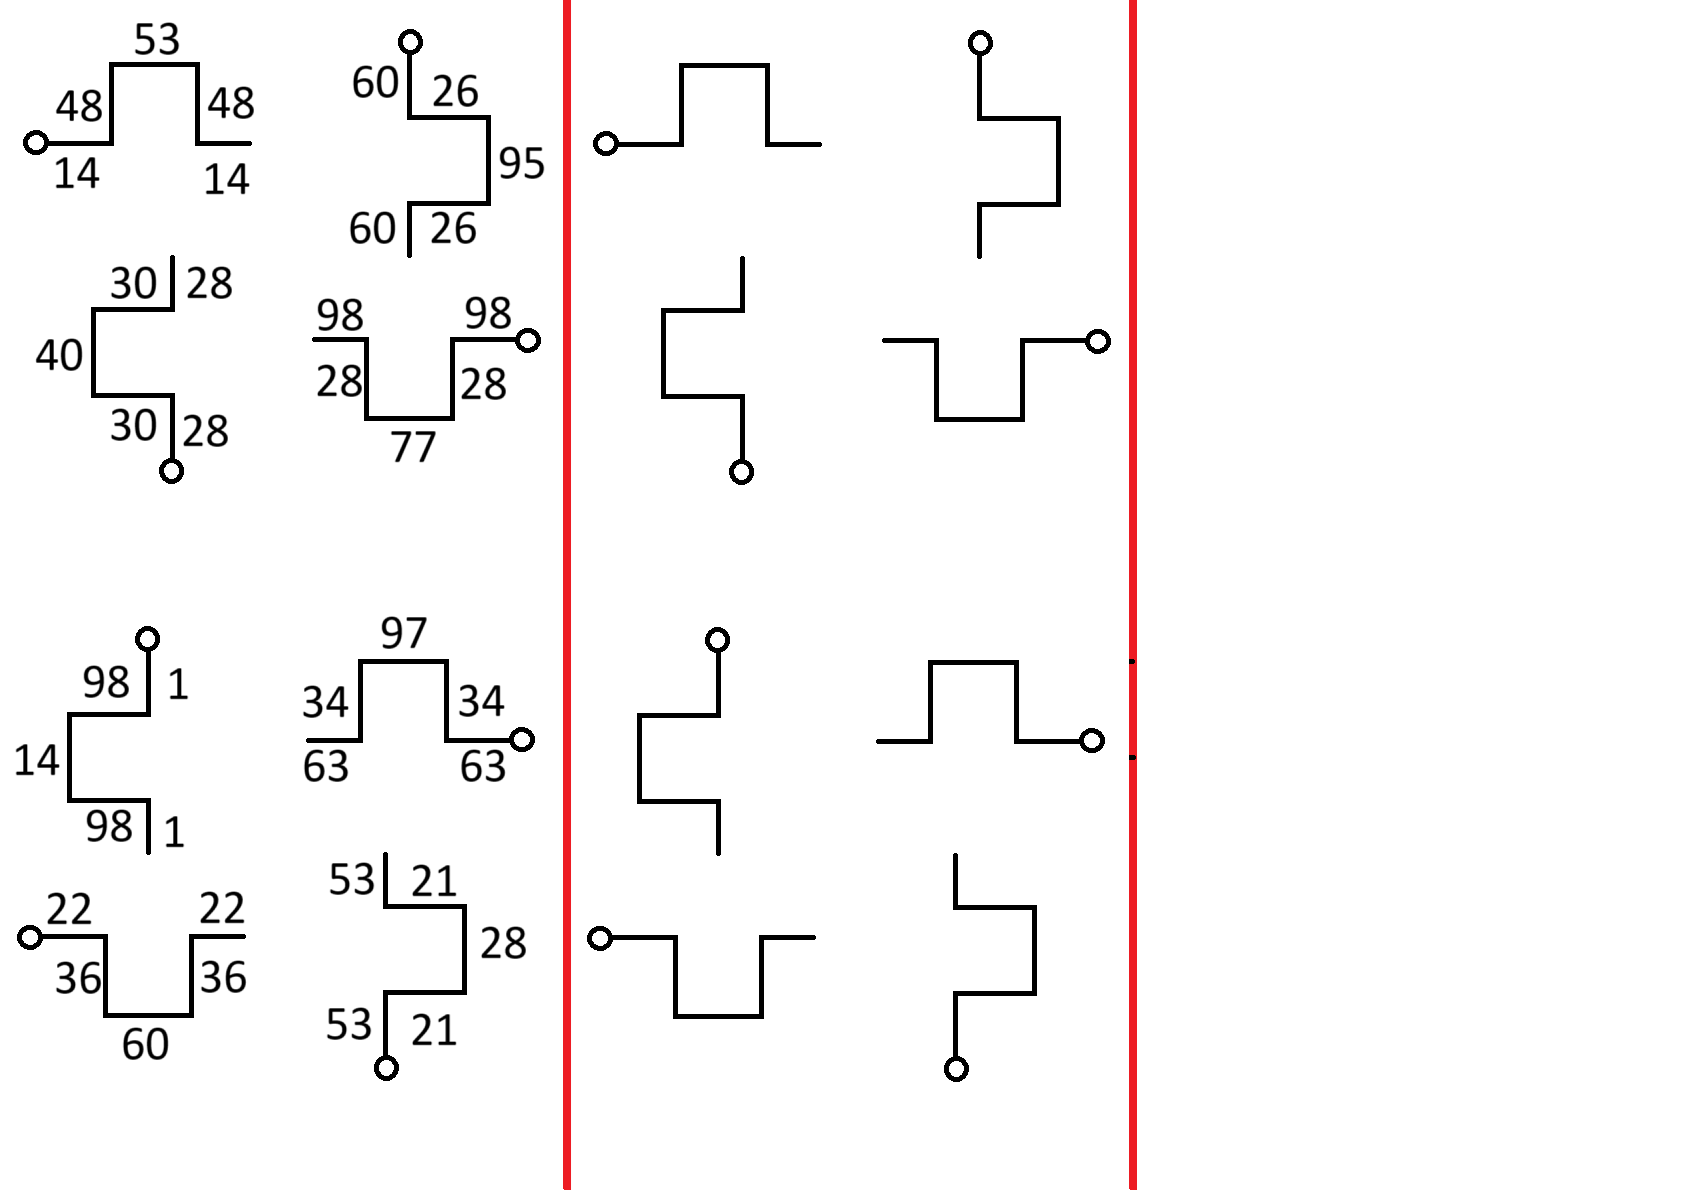
\includegraphics[width=\textwidth]{./figure/C413.png}}
    \caption{C413}
    \label{fig:C413:origin}
  \end{subfigure}

  \vspace{0.5cm}

  \begin{subfigure}[b]{0.3\textwidth}
    \fbox{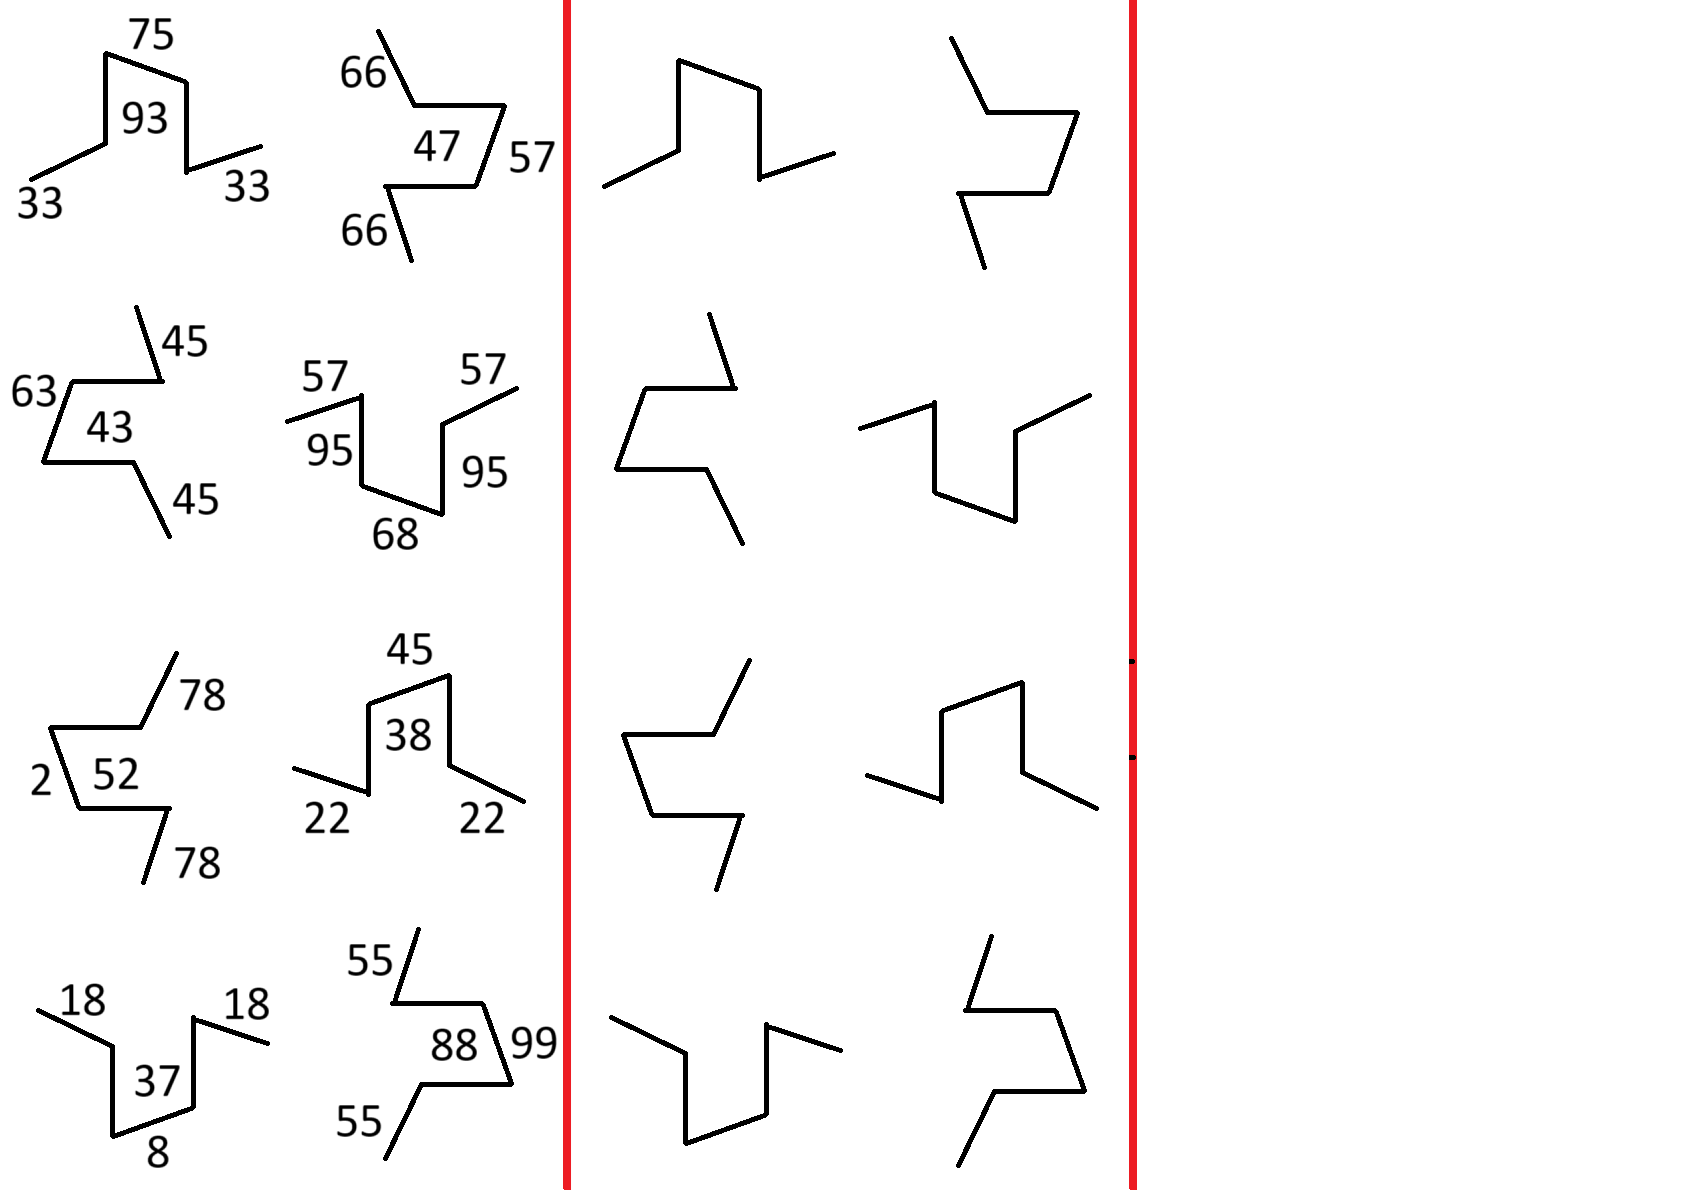
\includegraphics[width=\textwidth]{./figure/C445.png}}
    \caption{C445}
    \label{fig:C445:origin}
  \end{subfigure}
  \hfill
  \begin{subfigure}[b]{0.3\textwidth}
    \fbox{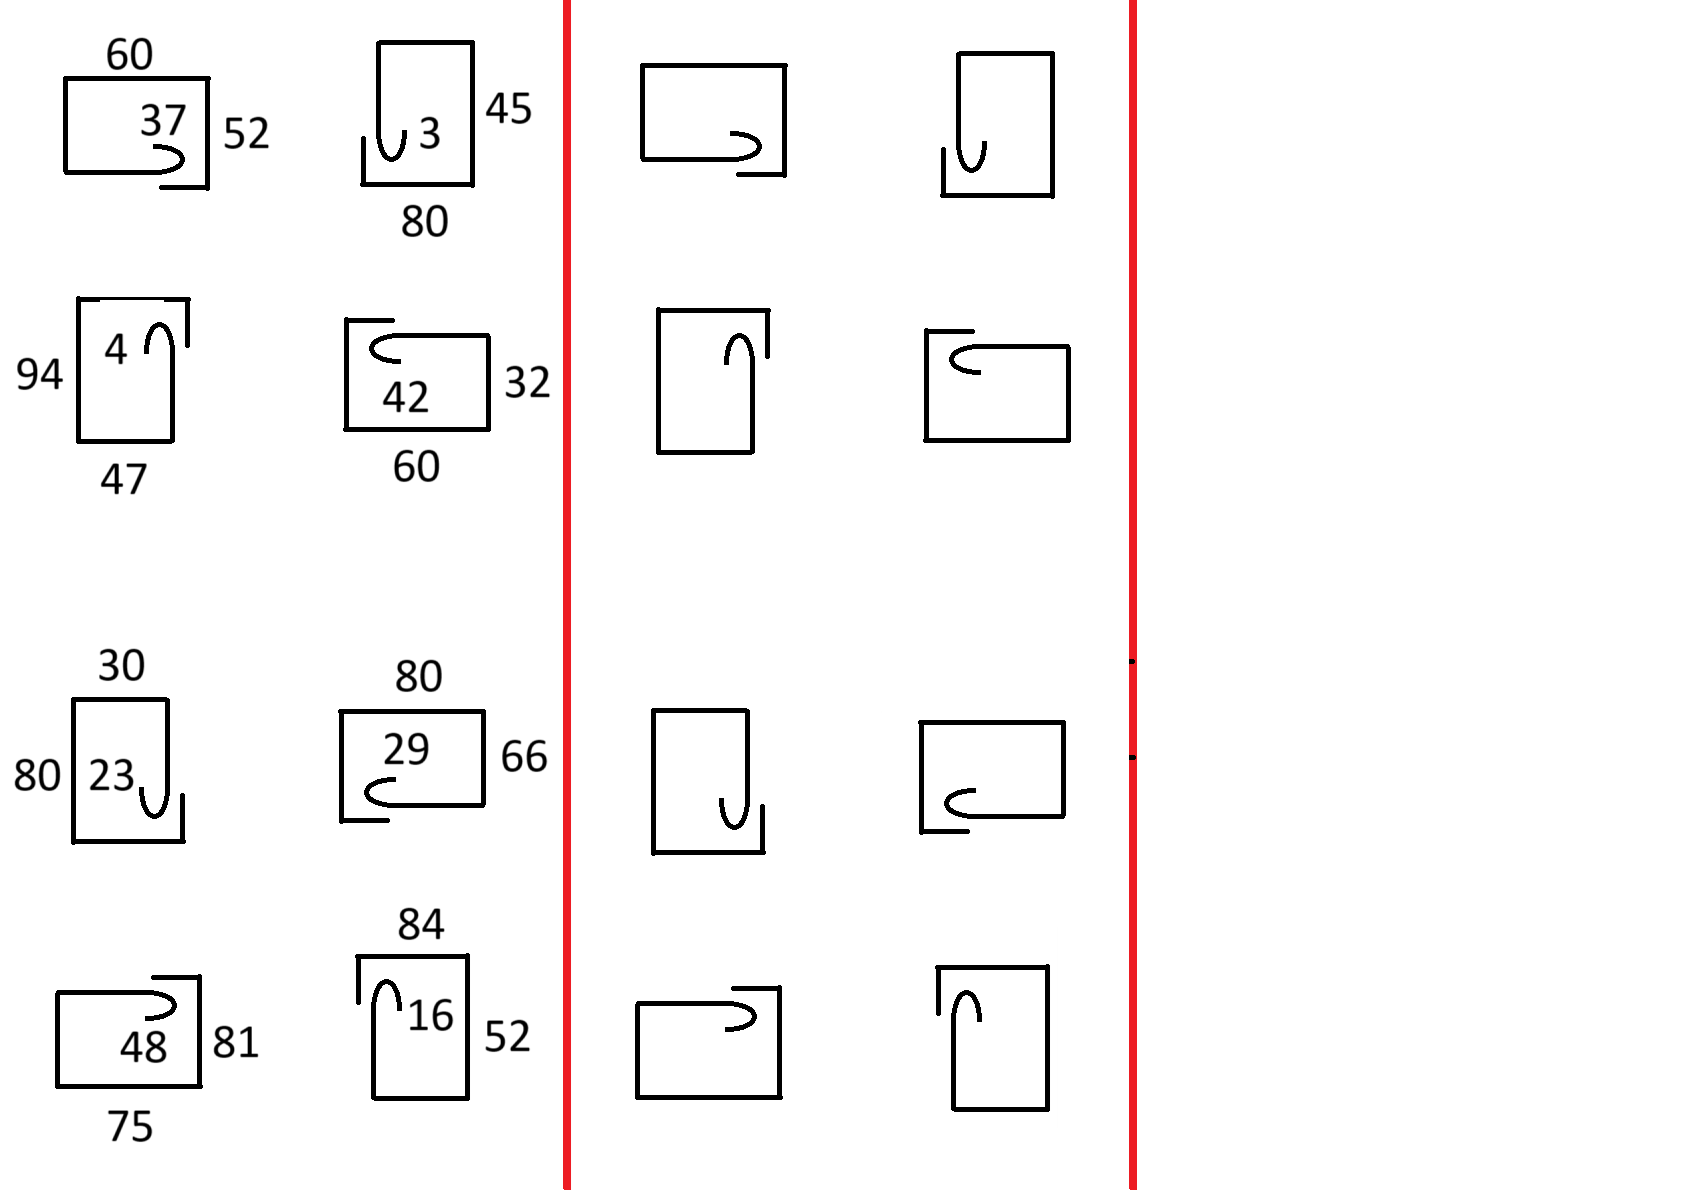
\includegraphics[width=\textwidth]{./figure/C505.png}}
    \caption{C505}
    \label{fig:C505:origin}
  \end{subfigure}
  \hfill
  \begin{subfigure}[b]{0.3\textwidth}
    \fbox{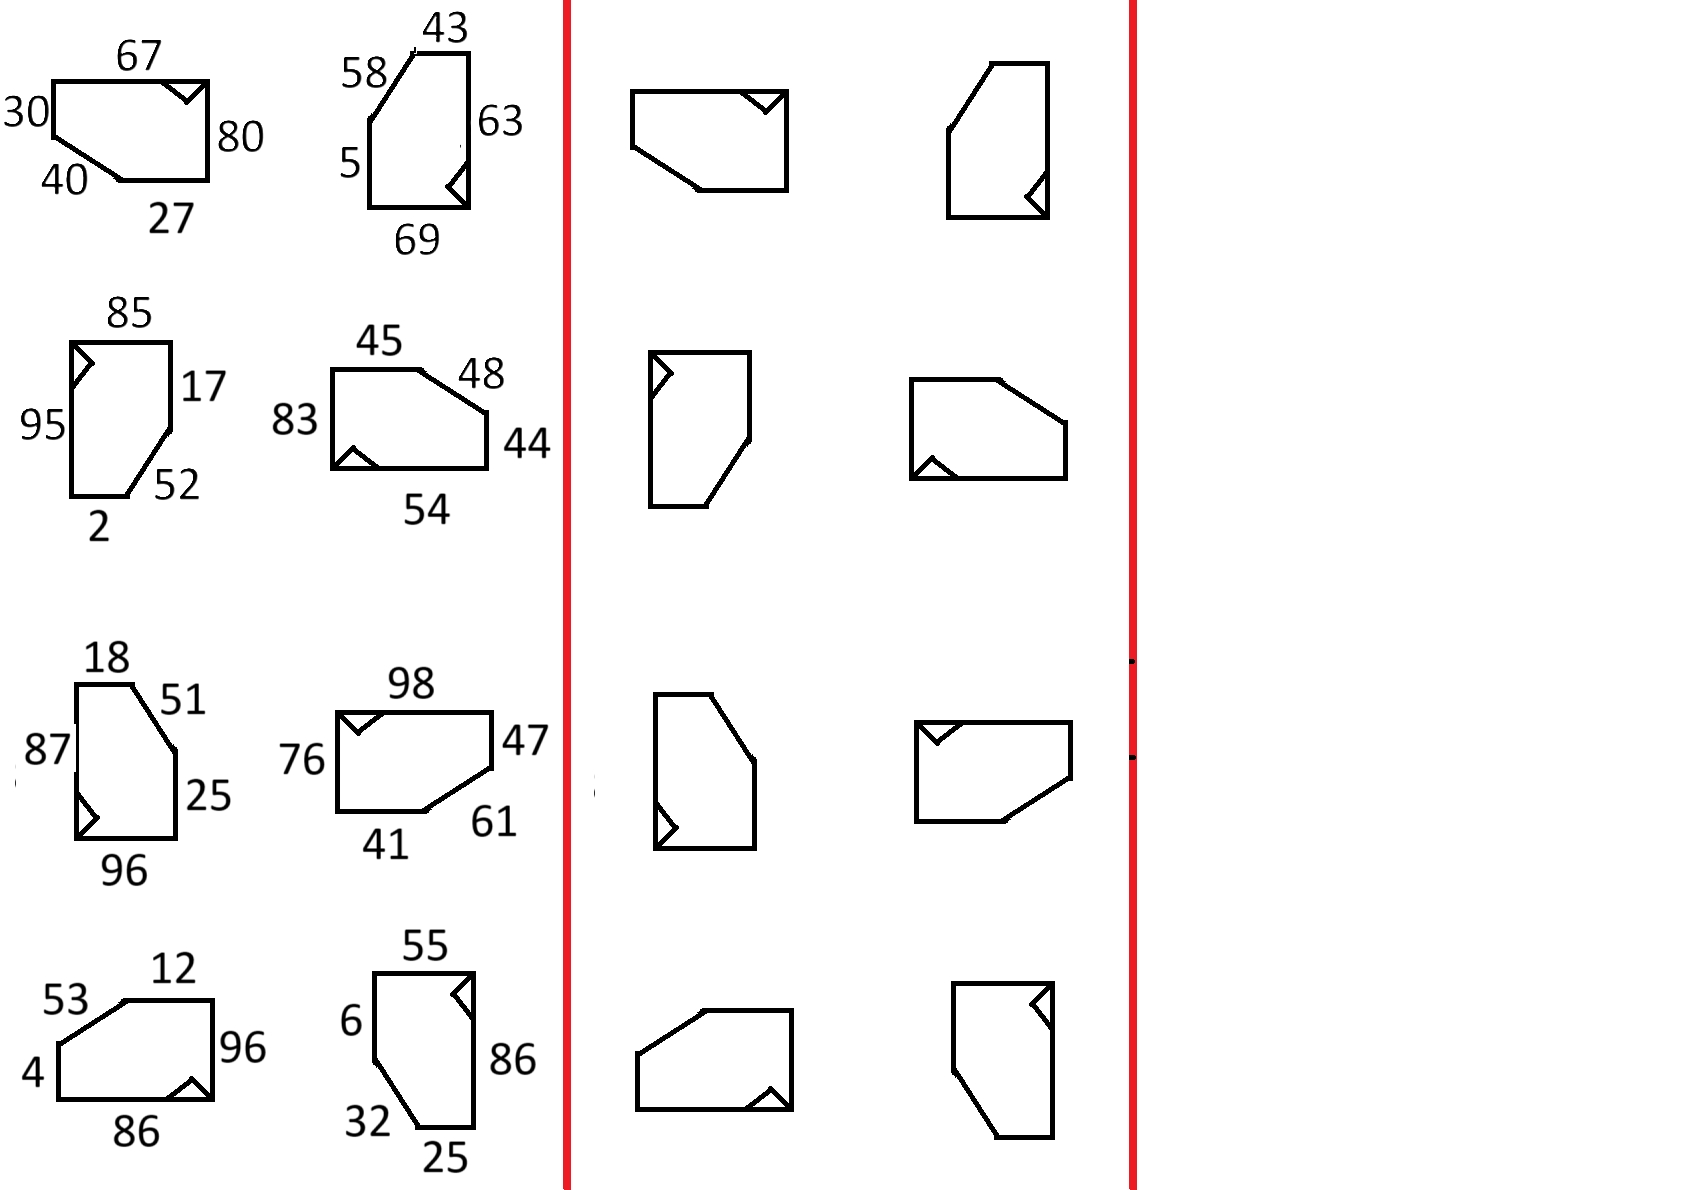
\includegraphics[width=\textwidth]{./figure/C603.png}}
    \caption{C603}
    \label{fig:C603:origin}
  \end{subfigure}

  \caption{Steel Shape Categories C105,C106,C413,C445,C505,C603 (with borders)}
  \label{fig:CXXX:origin}
\end{figure}

\subsection{填寫完的圖片}
\begin{figure}[H]
  \centering

  \begin{subfigure}[b]{0.3\textwidth}
    \fbox{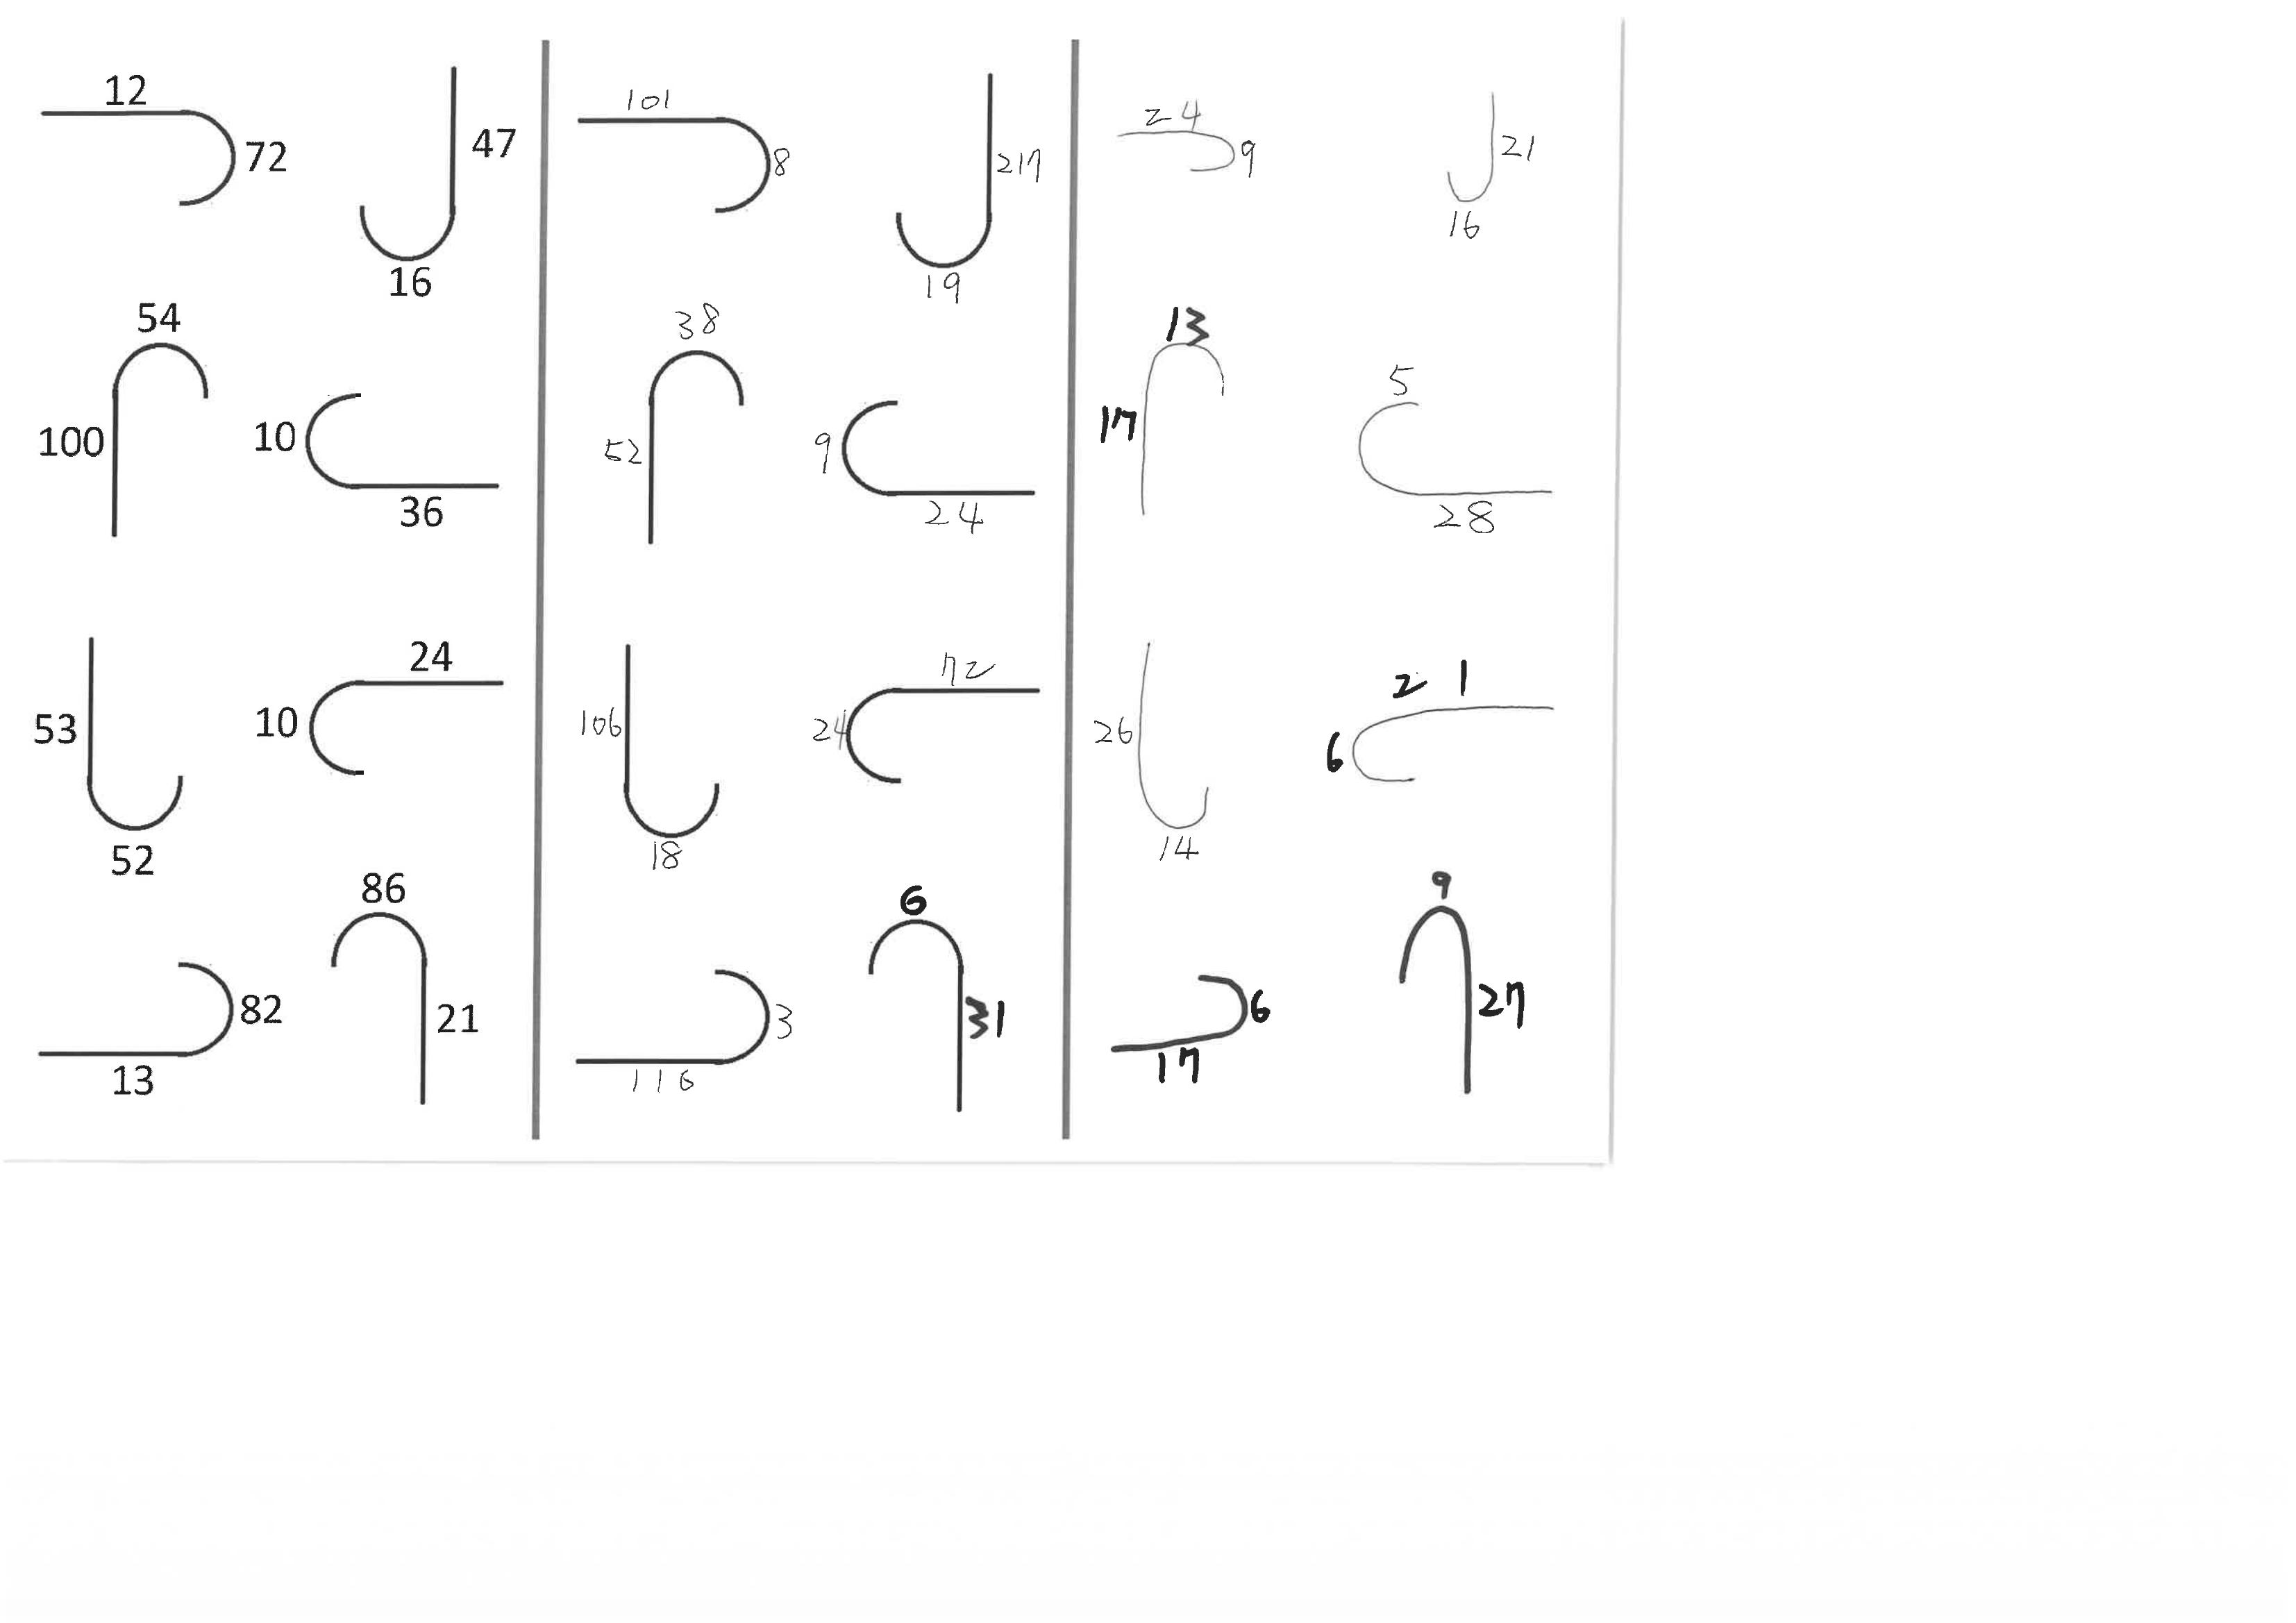
\includegraphics[width=\textwidth]{./figure/C105.jpeg}}
    \caption{C105}
    \label{fig:C105:done}
  \end{subfigure}
  \hfill
  \begin{subfigure}[b]{0.3\textwidth}
    \fbox{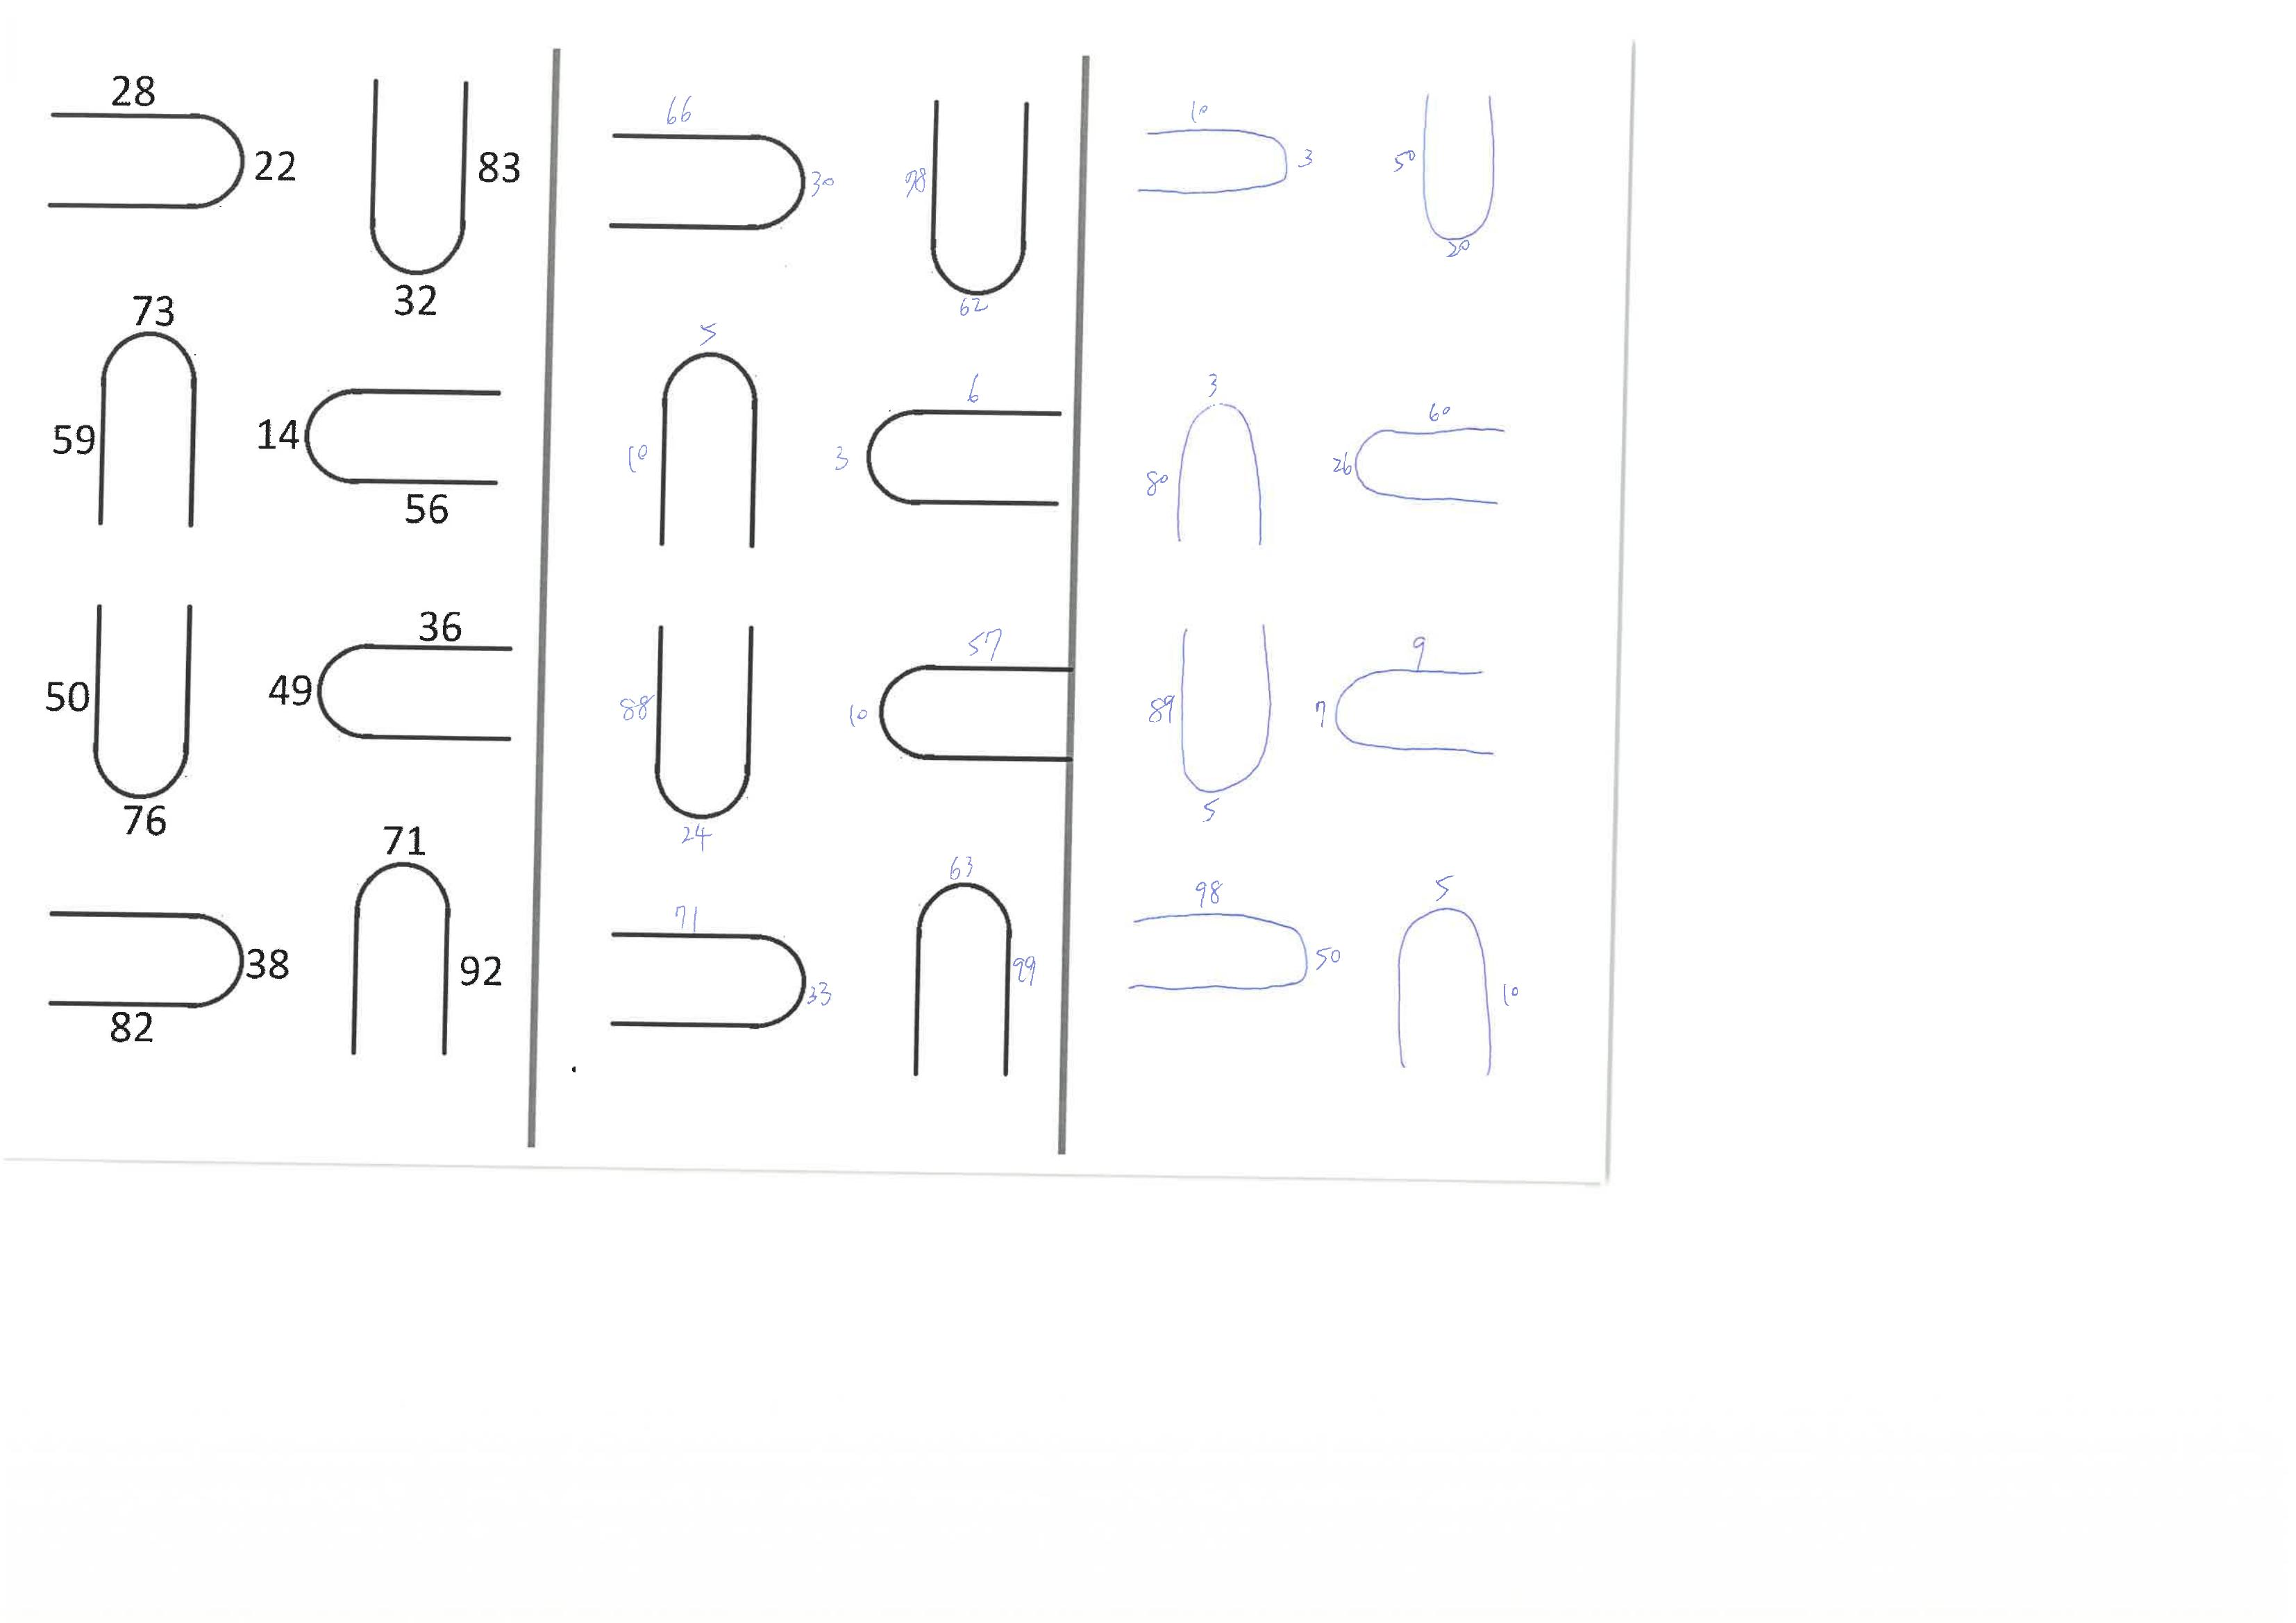
\includegraphics[width=\textwidth]{./figure/C106.jpeg}}
    \caption{C106}
    \label{fig:C106:done}
  \end{subfigure}
  \hfill
  \begin{subfigure}[b]{0.3\textwidth}
    \fbox{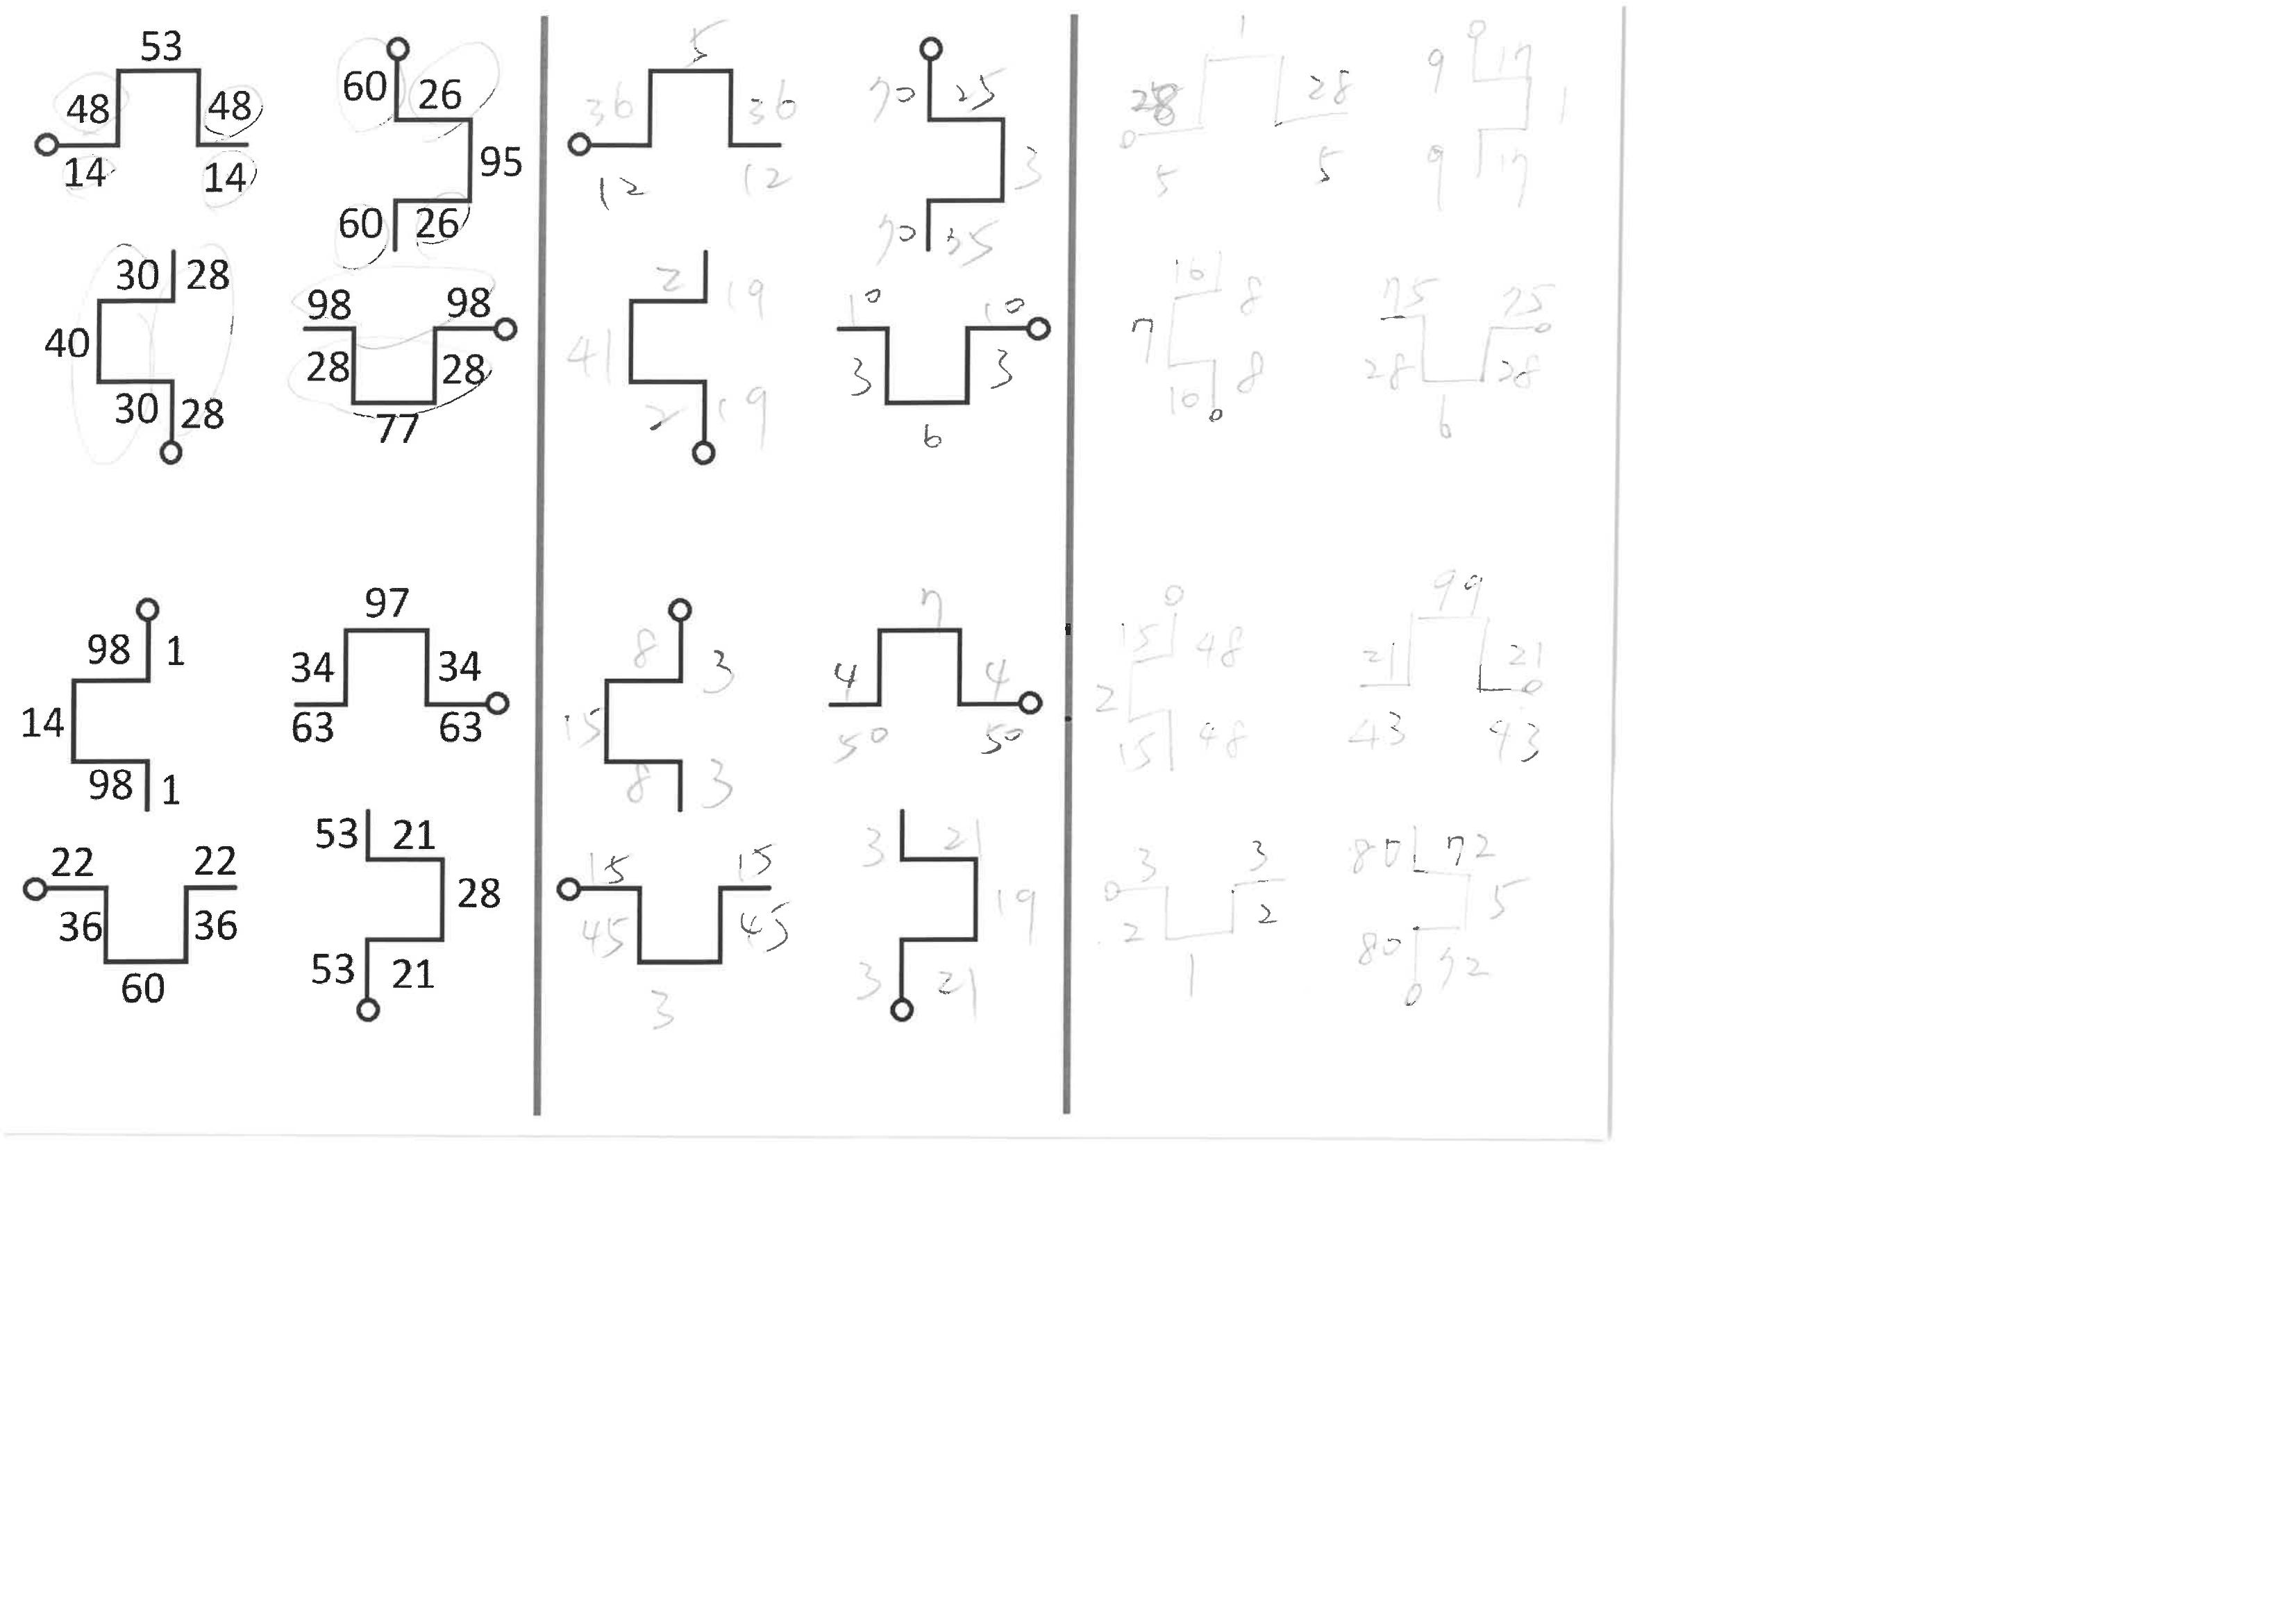
\includegraphics[width=\textwidth]{./figure/C413.jpeg}}
    \caption{C413}
    \label{fig:C413:done}
  \end{subfigure}

  \vspace{0.5cm}

  \begin{subfigure}[b]{0.3\textwidth}
    \fbox{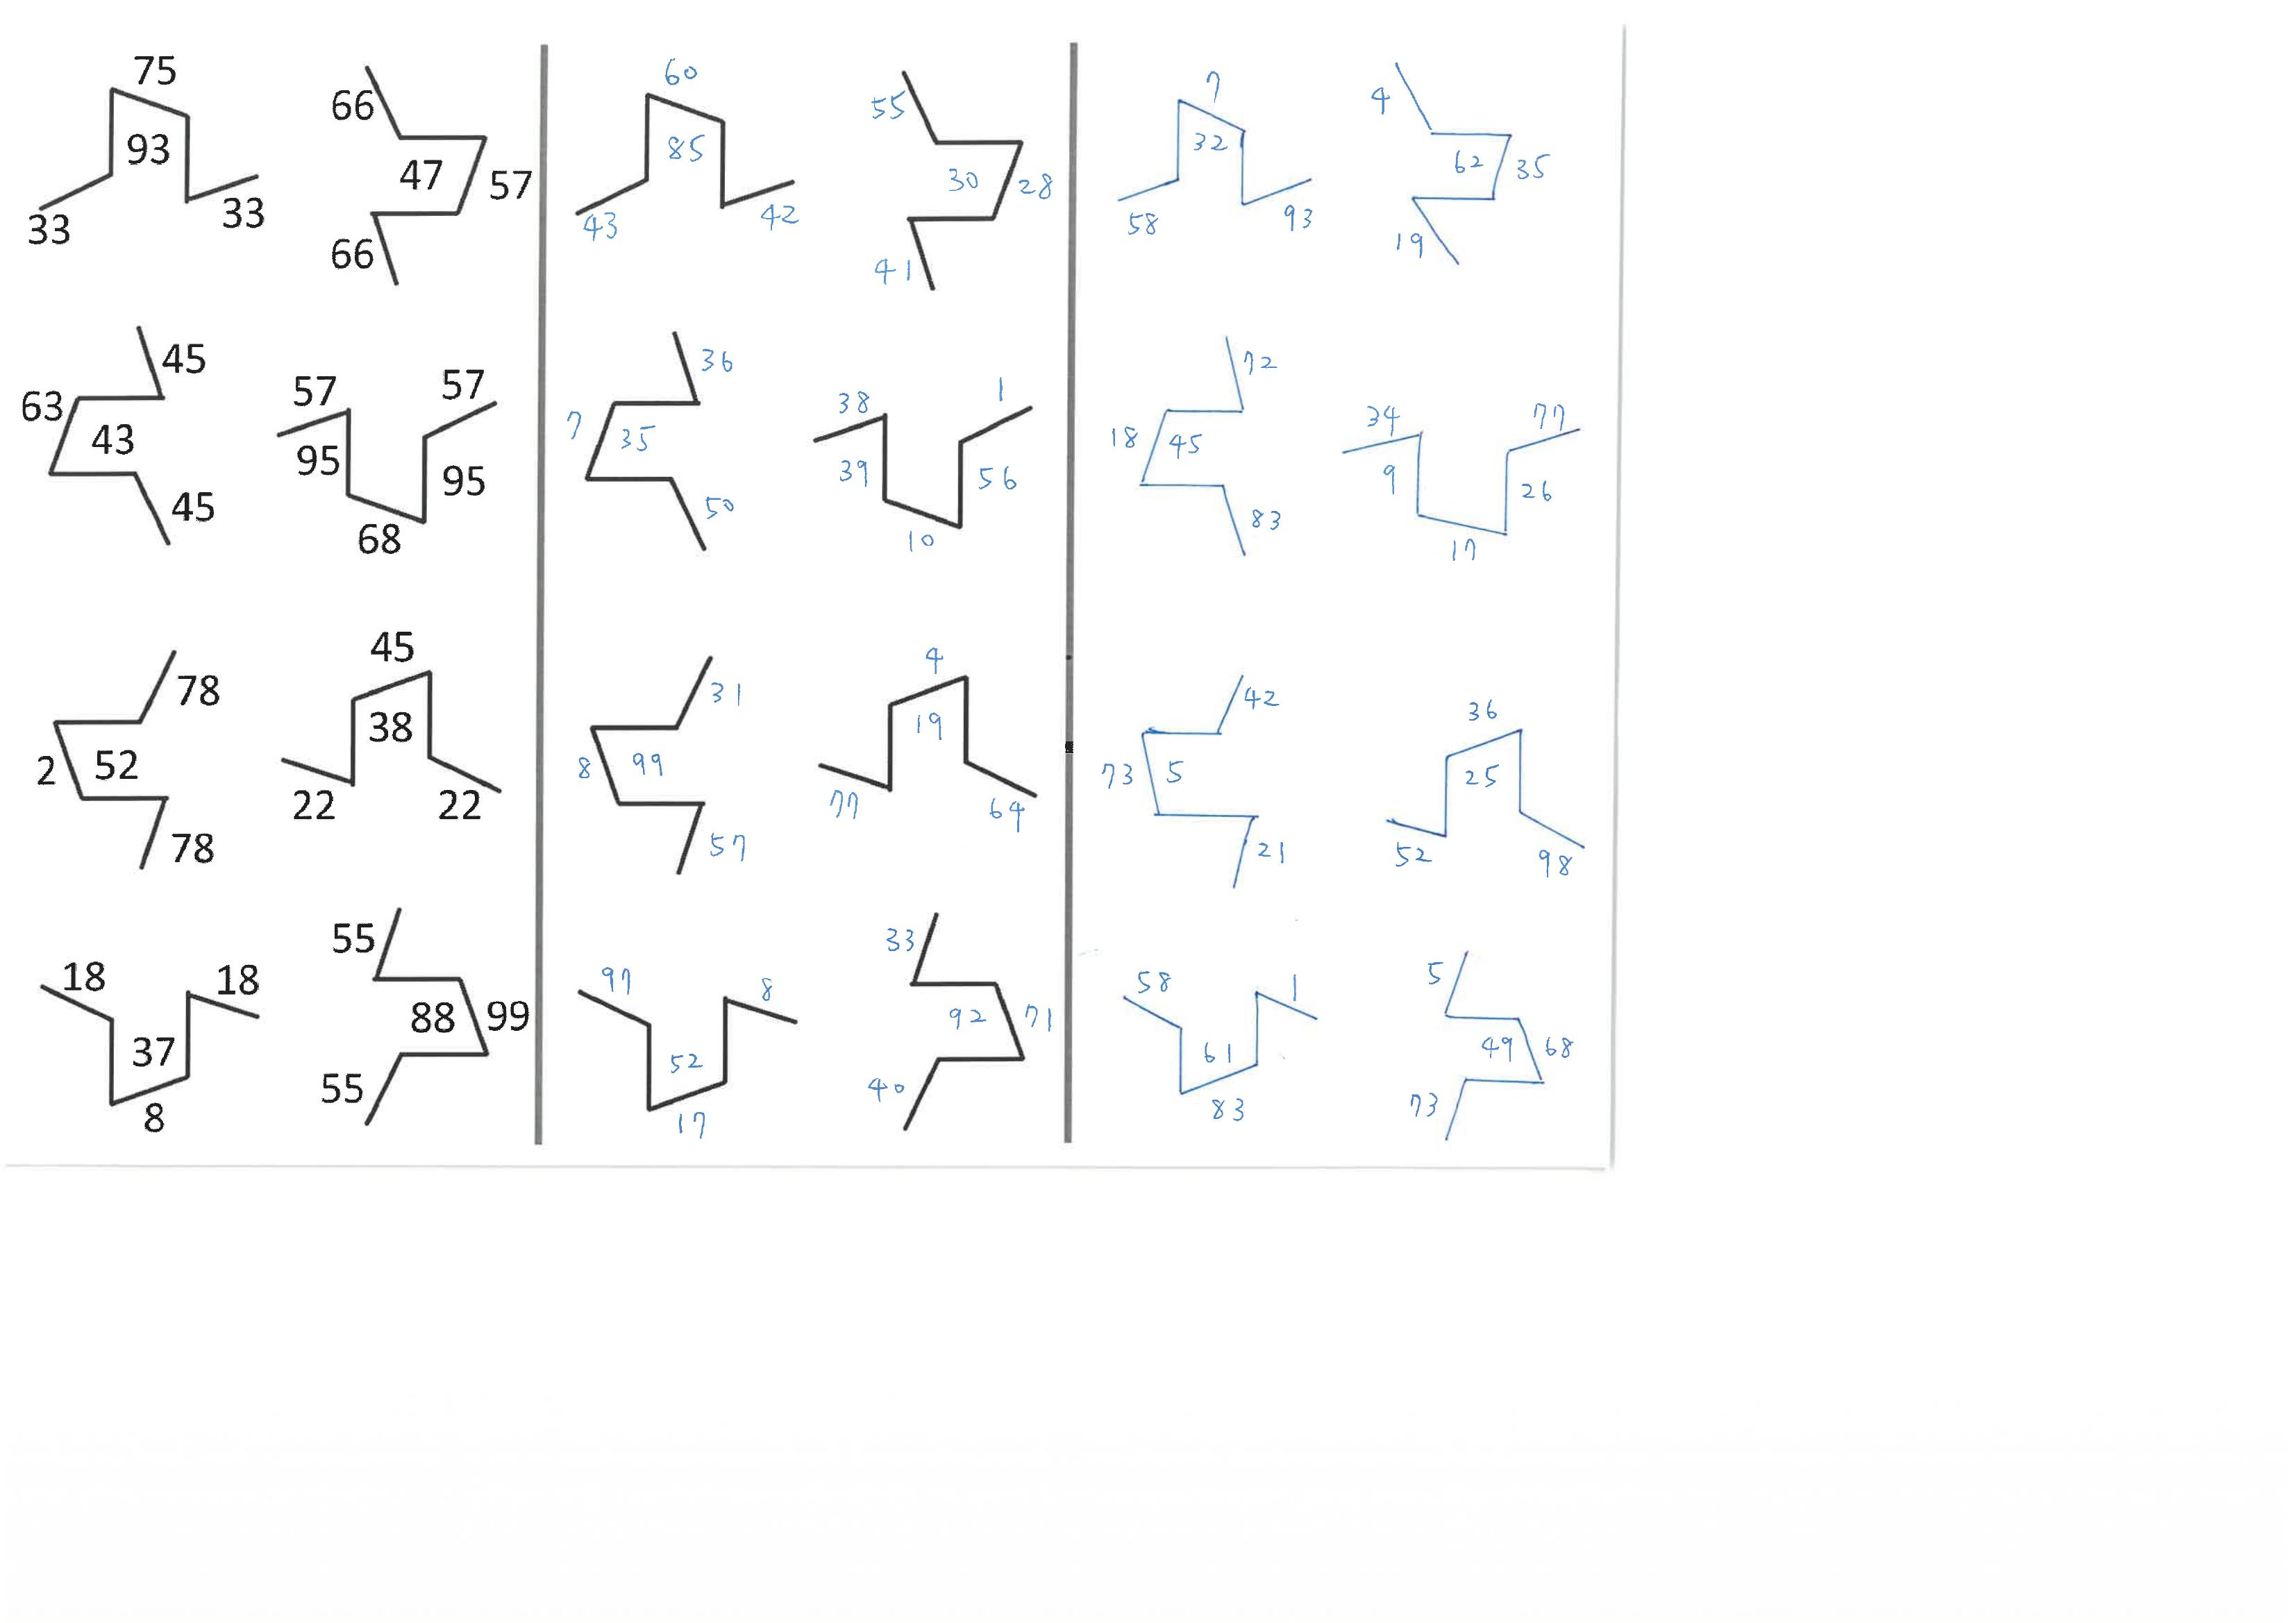
\includegraphics[width=\textwidth]{./figure/C445.jpeg}}
    \caption{C445}
    \label{fig:C445:done}
  \end{subfigure}
  \hfill
  \begin{subfigure}[b]{0.3\textwidth}
    \fbox{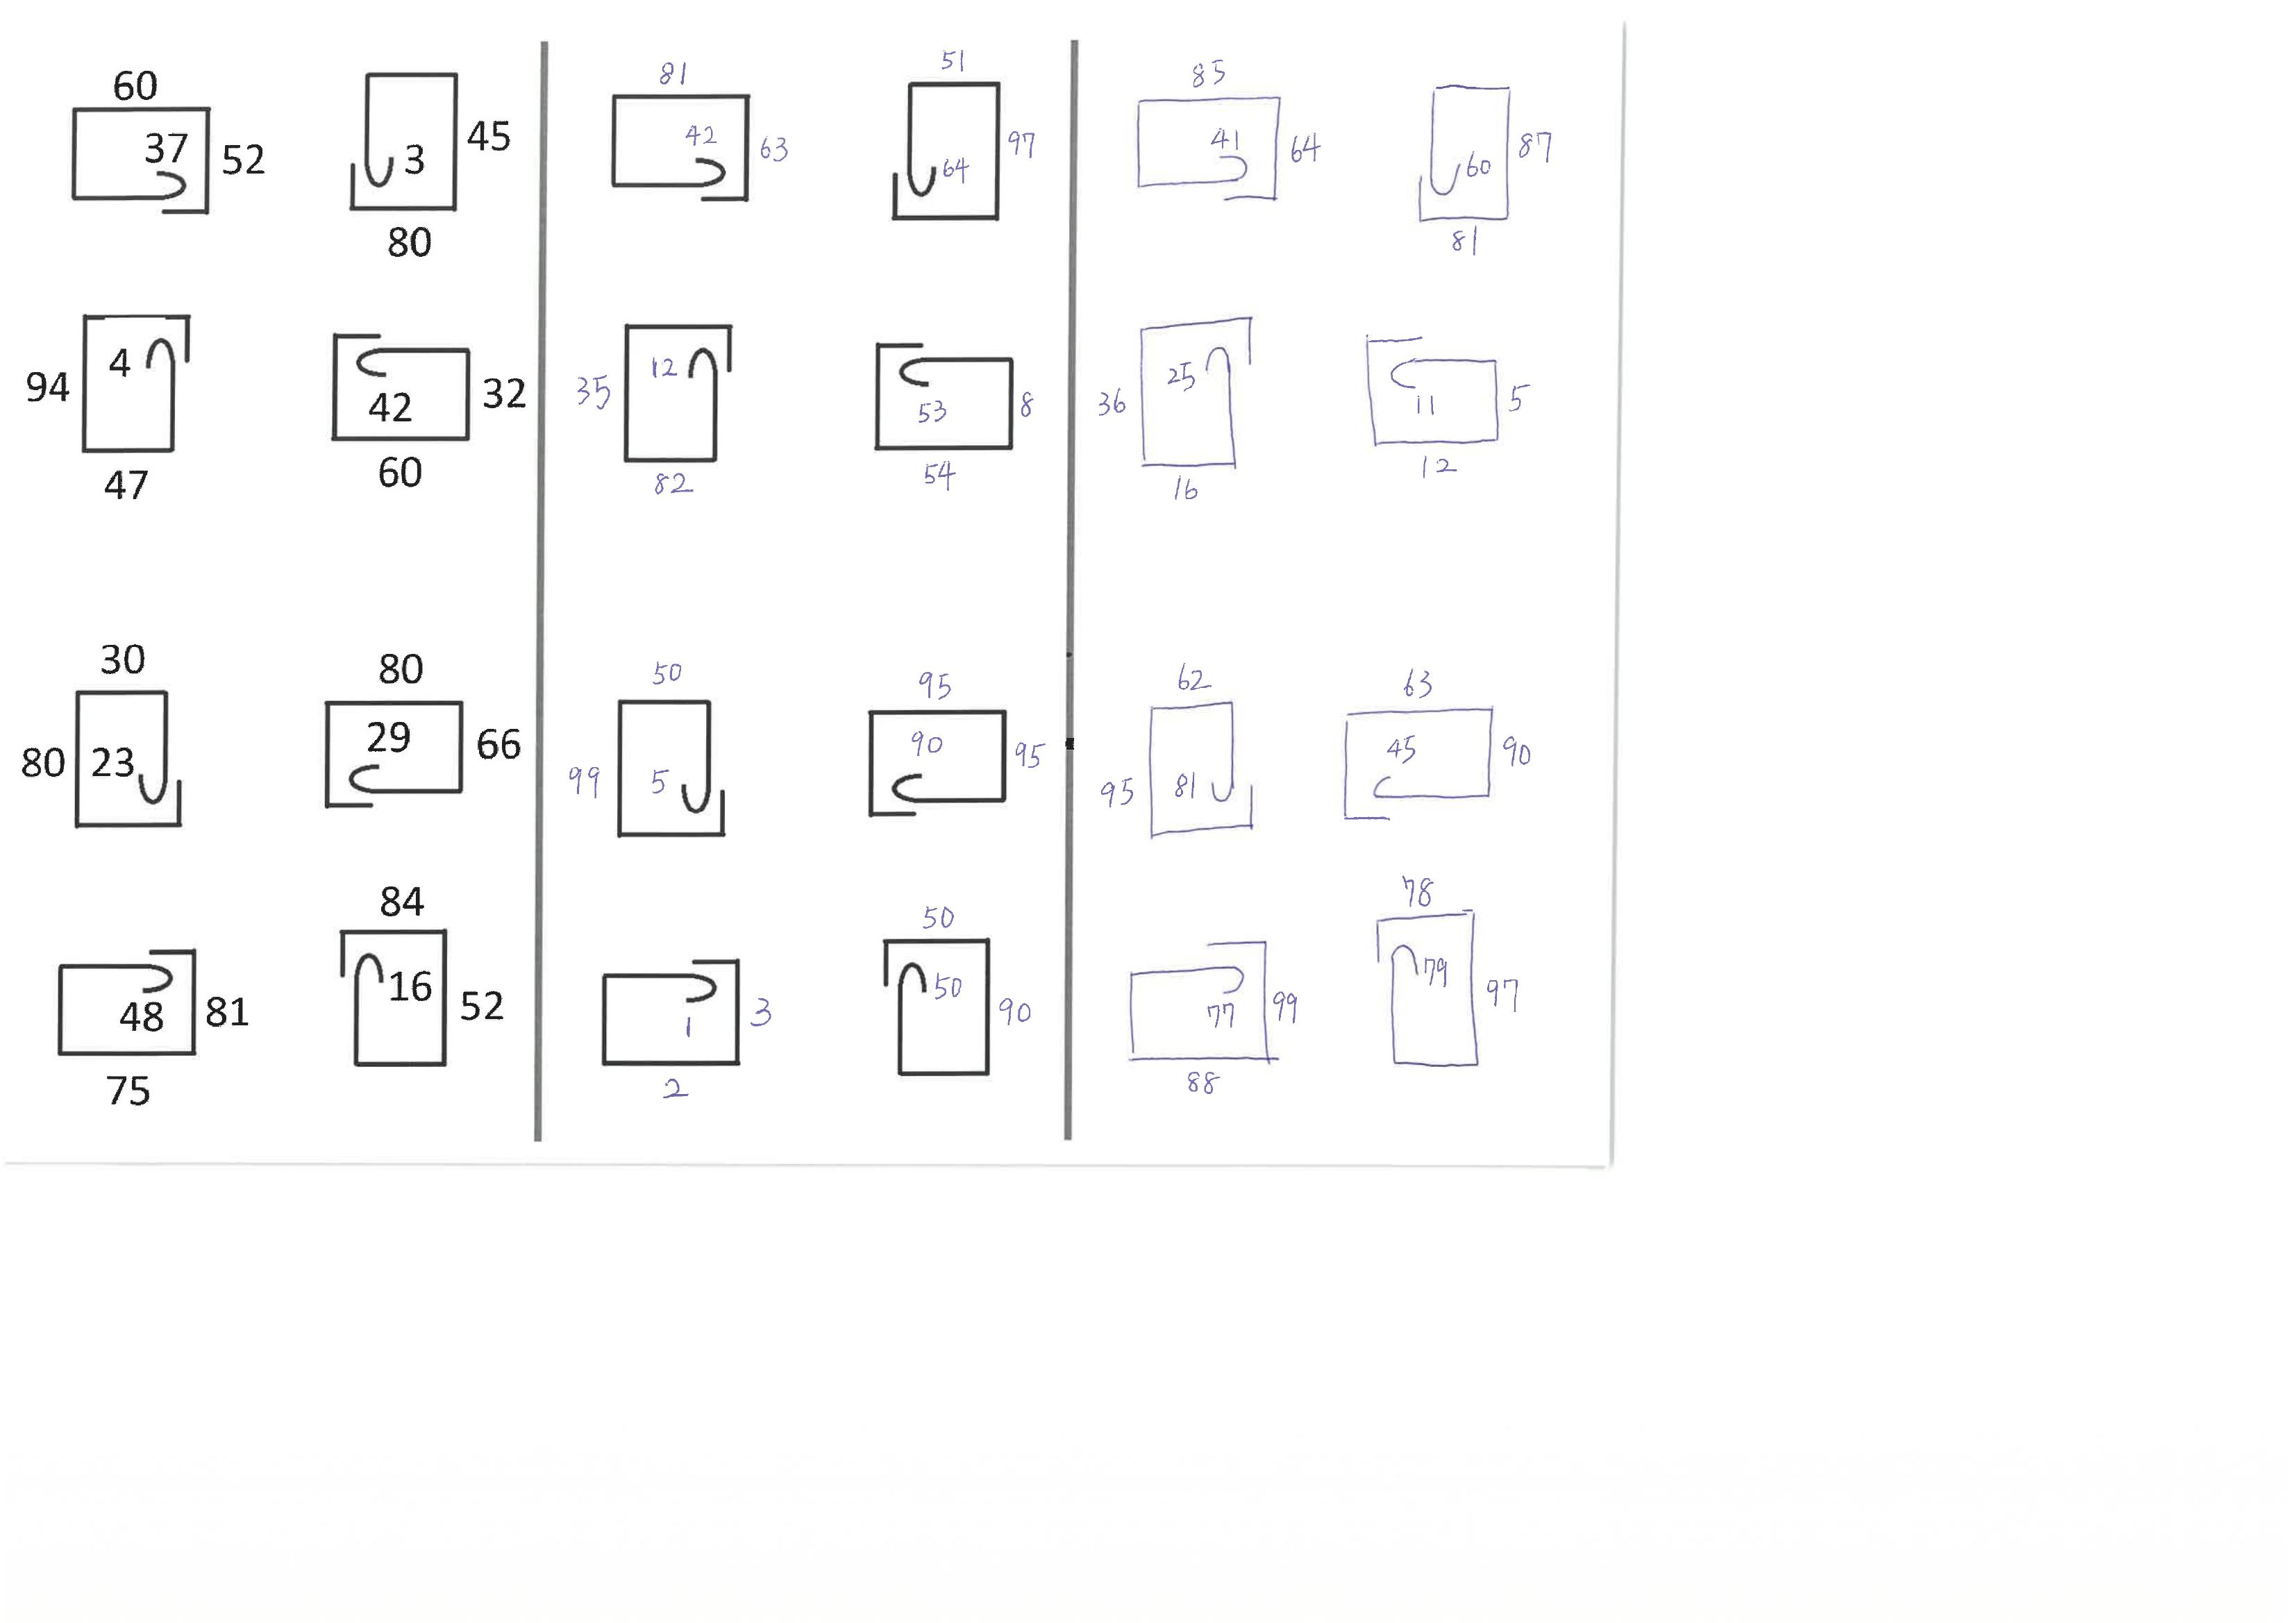
\includegraphics[width=\textwidth]{./figure/C505.jpeg}}
    \caption{C505}
    \label{fig:C505:done}
  \end{subfigure}
  \hfill
  \begin{subfigure}[b]{0.3\textwidth}
    \fbox{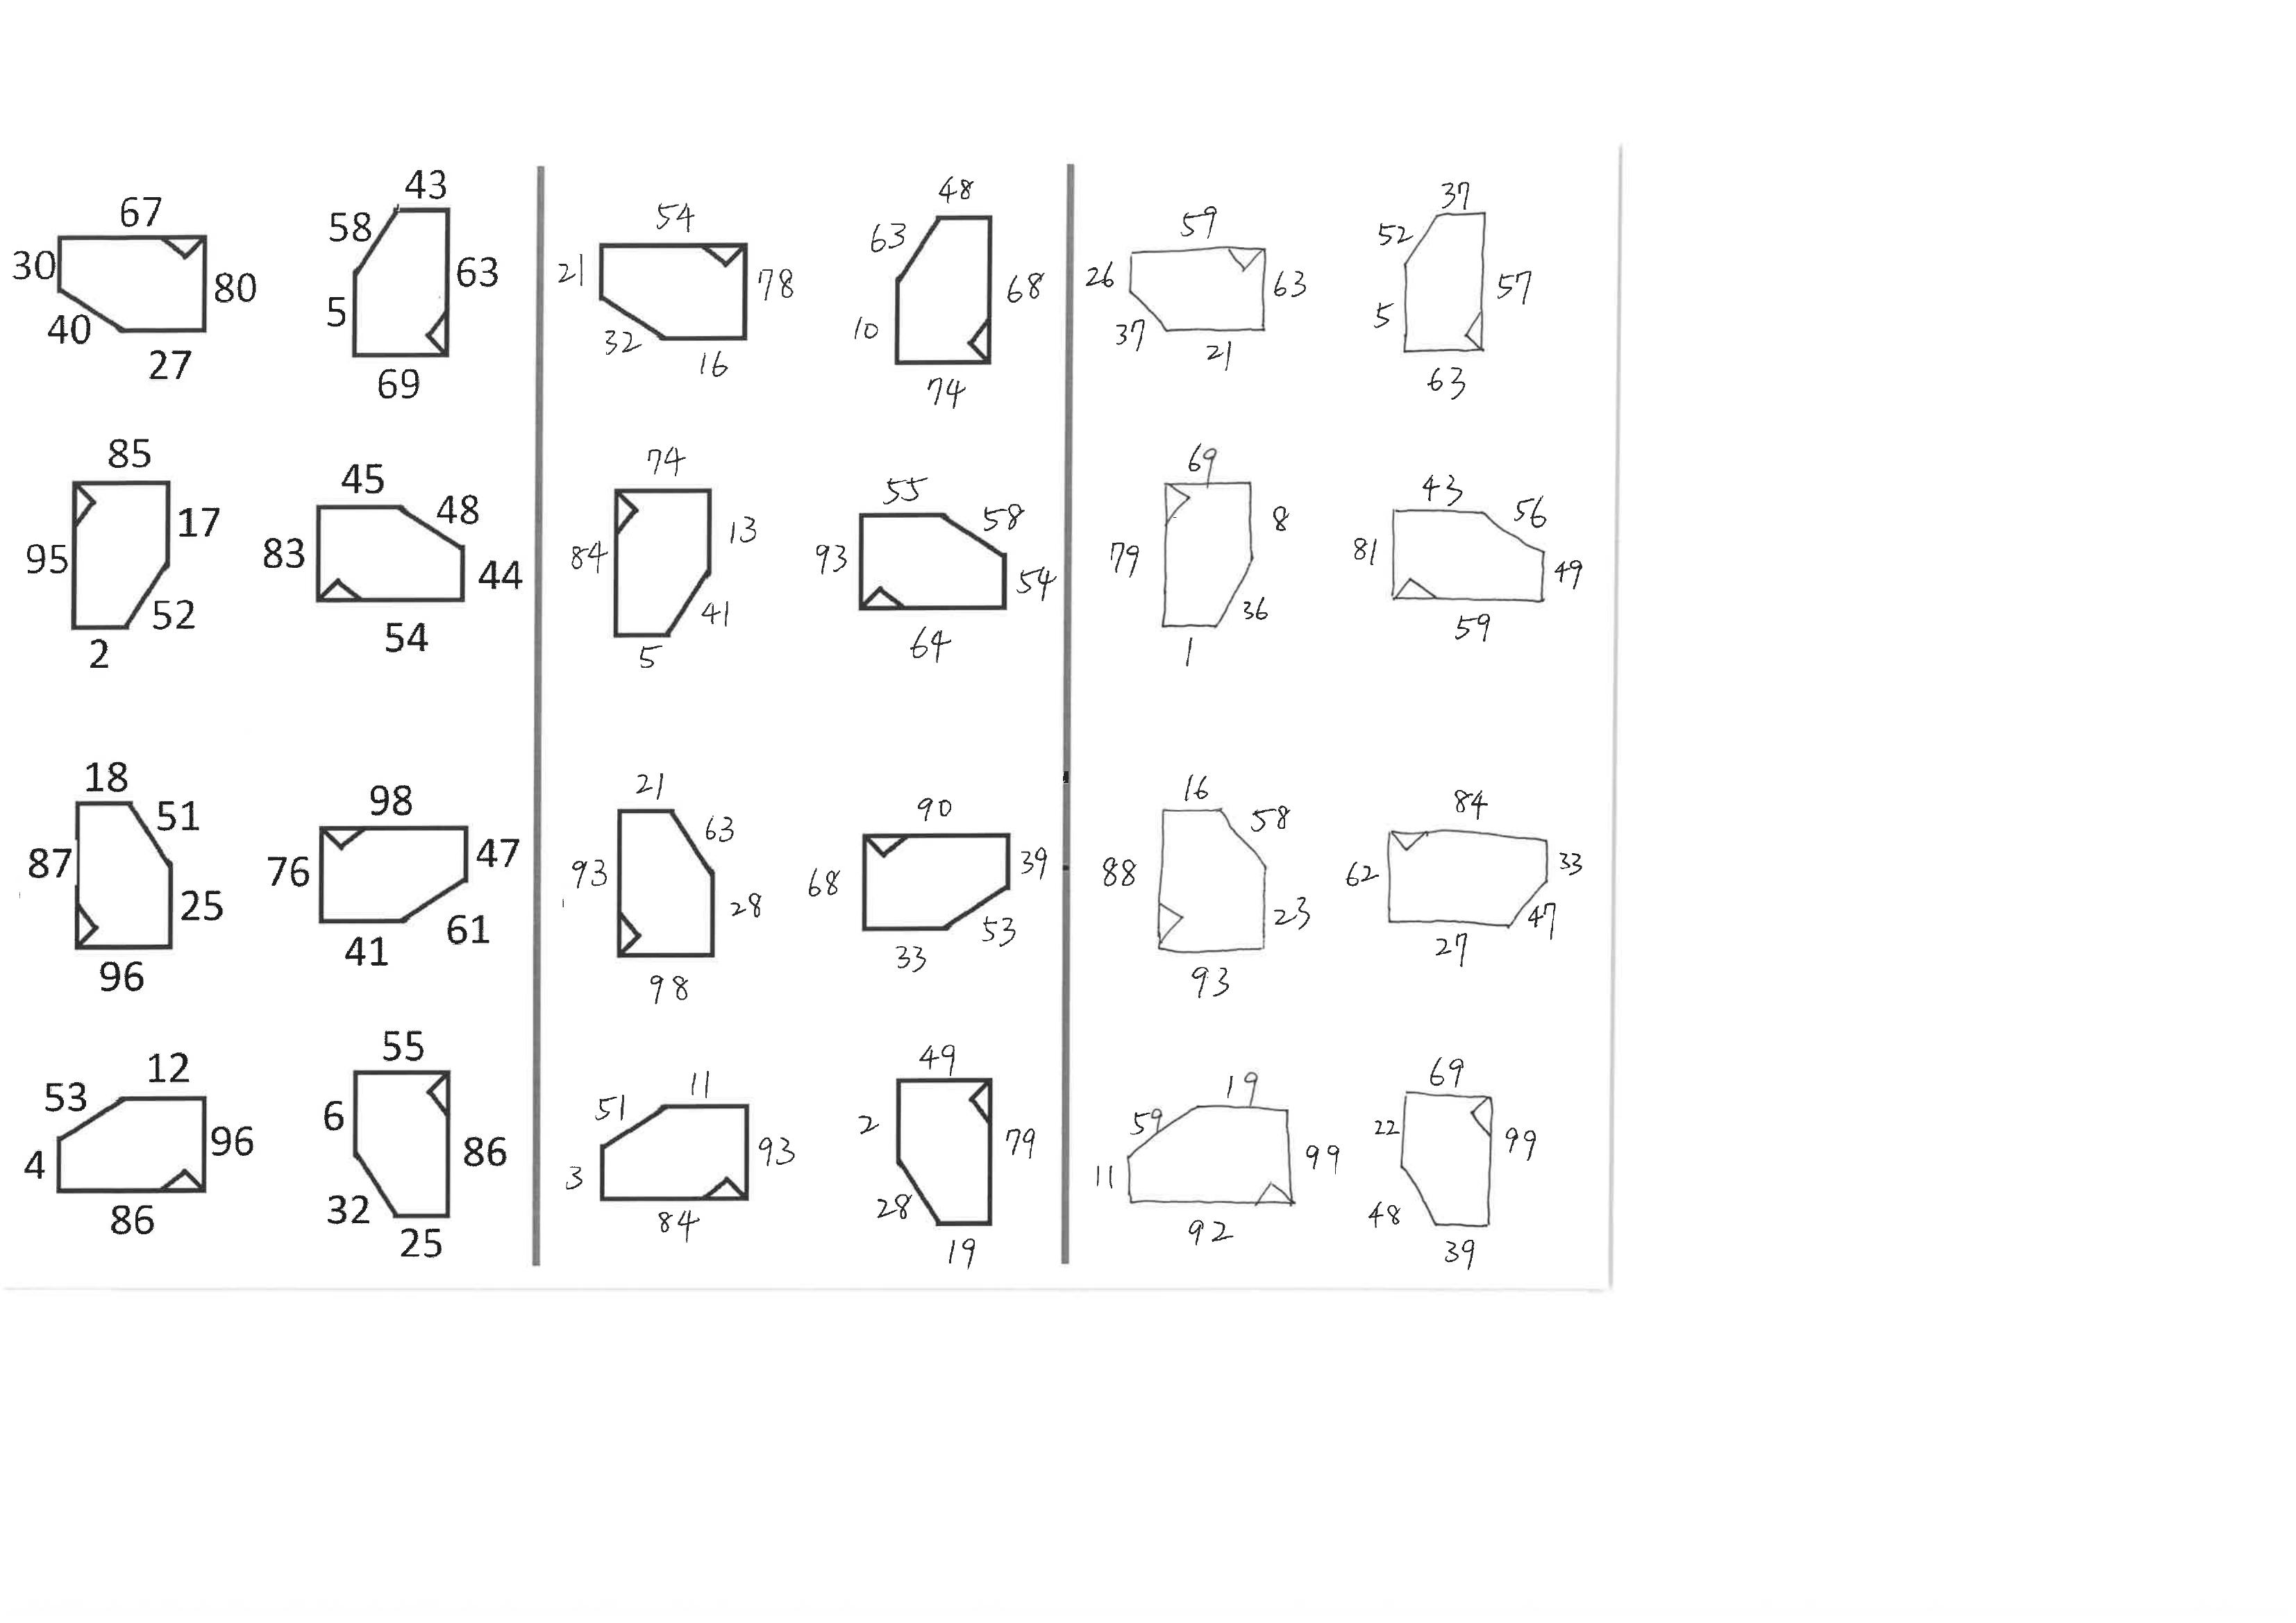
\includegraphics[width=\textwidth]{./figure/C603.jpeg}}
    \caption{C603}
    \label{fig:C603:done}
  \end{subfigure}

  \caption{Steel Shape Categories C105,C106,C413,C445,C505,C603 (with borders)}
  \label{fig:CXXX:done}
\end{figure}

\subsection{分割, 以C105舉例}
\begin{figure}[H]
  \centering
  % 圖片 1~24, 每行 6 張圖
  \foreach \i in {1,...,24} {
    \begin{subfigure}[b]{0.15\textwidth}
      \fbox{\includegraphics[width=\textwidth]{./figure/C105_\i.png}}
      \caption*{\scriptsize C105\_\i}
    \end{subfigure}
    \ifnum\i=6 \par\medskip\fi
    \ifnum\i=12 \par\medskip\fi
    \ifnum\i=18 \par\medskip\fi
  }

  \caption{Subcomponents of Steel Shape C105 (1–24)}
  \label{fig:C105:all}
\end{figure}

\subsection{旋轉以及翻轉, 以C105\_1舉例}

\begin{figure}[H]
  \centering
  \foreach \img/\cap in {
    C105_1_rot0/rot0,
    C105_1_rot1/rot1,
    C105_1_rot2/rot2,
    C105_1_rot3/rot3,
    C105_1_flip_rot0/flip\_rot0,
    C105_1_flip_rot1/flip\_rot1,
    C105_1_flip_rot2/flip\_rot2,
    C105_1_flip_rot3/flip\_rot3
  } {
    \begin{subfigure}[b]{0.22\textwidth}
      \centering
      \fbox{%
        \includegraphics[width=3.5cm,height=3.5cm,keepaspectratio]{./figure/\img.png}
      }
      \caption*{\scriptsize \cap}
    \end{subfigure}
    \hfill
  }

  \caption{C105\_1 不同旋轉與翻轉版本(共 8 張)}
  \label{fig:C105_1_variants}
\end{figure}

\section{image prompt 增強}
\begin{figure}[H]
  \centering
  \fbox{%
    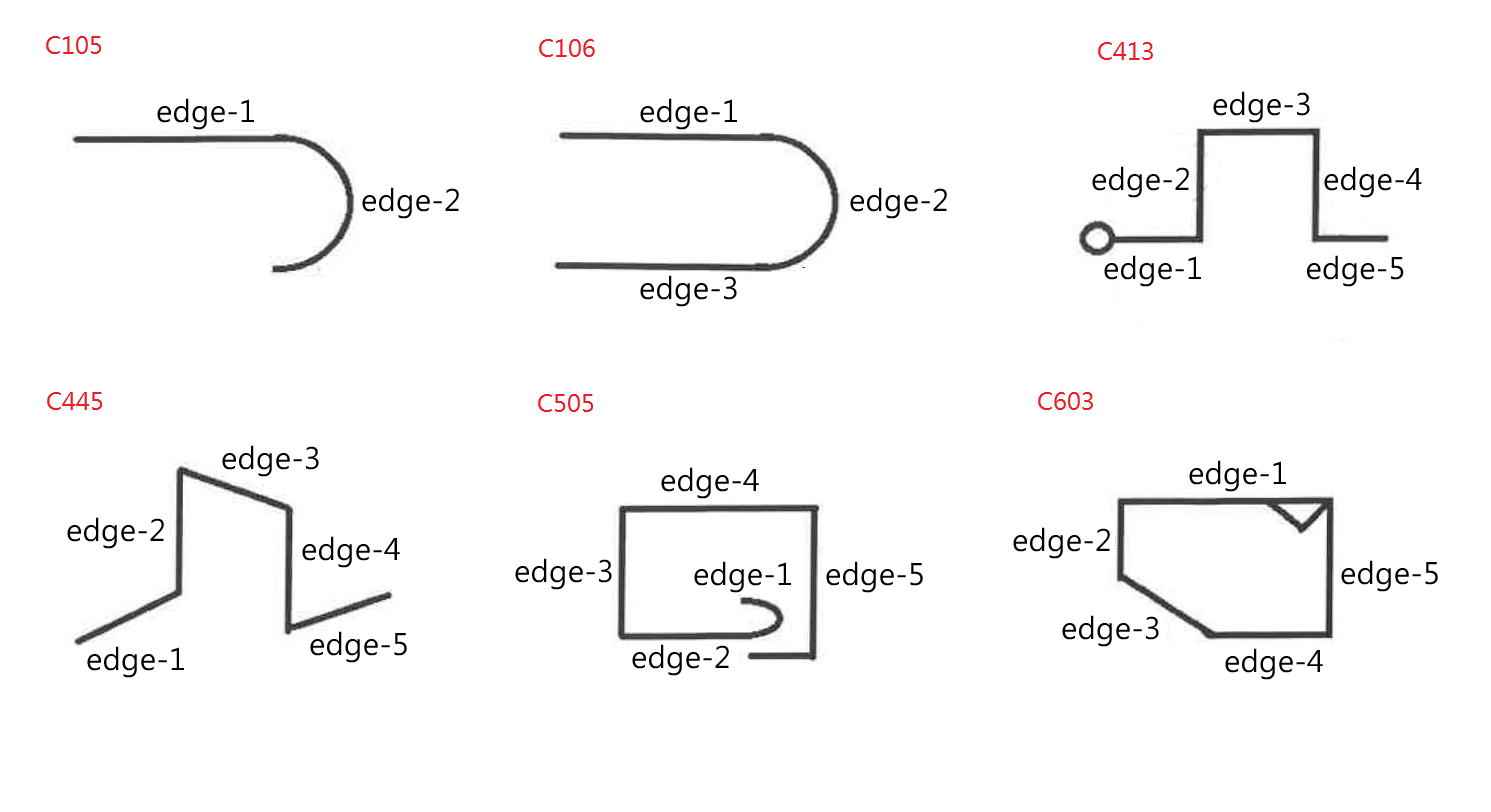
\includegraphics[width=0.95\textwidth]{./figure/full_image.png}
  }
  \caption{image prompt 增強}
  \label{fig:full_image}
\end{figure}
\section{模型準確率以及損失}
\begin{figure}[H]
  \centering

  \begin{subfigure}[b]{0.45\textwidth}
    \fbox{\includegraphics[width=\textwidth]{figure/model0_loss_acc.png}}
    \caption{Model 0 Loss/Accuracy}
    \label{fig:model0:lossacc}
  \end{subfigure}
  \hfill
  \begin{subfigure}[b]{0.45\textwidth}
    \fbox{\includegraphics[width=\textwidth]{figure/model1_loss_acc.png}}
    \caption{Model 1 Loss/Accuracy}
    \label{fig:model1:lossacc}
  \end{subfigure}

  \vspace{0.5cm}

  \begin{subfigure}[b]{0.45\textwidth}
    \fbox{\includegraphics[width=\textwidth]{figure/model2_loss_acc.png}}
    \caption{Model 2 Loss/Accuracy}
    \label{fig:model2:lossacc}
  \end{subfigure}
  \hfill
  \begin{subfigure}[b]{0.45\textwidth}
    \fbox{\includegraphics[width=\textwidth]{figure/model3_loss_acc.png}}
    \caption{Model 3 Loss/Accuracy}
    \label{fig:model3:lossacc}
  \end{subfigure}

  \caption{Training Loss and Accuracy Curves for Model 0–3}
  \label{fig:training-curves}
\end{figure}
\section{實驗結果}
\subsection{0}
{\footnotesize
  \begin{longtable}{>{\raggedright\arraybackslash}p{5cm}rrrrrr}
\toprule
tag & total\_count & json\_correct & structure\_correct & type\_correct & edge\_correct & all\_correct \\
\midrule
\endfirsthead
\toprule
tag & total\_count & json\_correct & structure\_correct & type\_correct & edge\_correct & all\_correct \\
\midrule
\endhead
\midrule
\multicolumn{7}{r}{Continued on next page} \\
\midrule
\endfoot
\bottomrule
\endlastfoot
C105|flip|handwritten\_only|rot0|test & 8 & 3 (37.50\%) & 3 (37.50\%) & 1 (12.50\%) & 0 (0.00\%) & 0 (0.00\%) \\
C105|flip|handwritten\_only|rot1|test & 8 & 6 (75.00\%) & 6 (75.00\%) & 1 (12.50\%) & 0 (0.00\%) & 0 (0.00\%) \\
C105|flip|handwritten\_only|rot2|test & 8 & 8 (100.00\%) & 8 (100.00\%) & 4 (50.00\%) & 0 (0.00\%) & 0 (0.00\%) \\
C105|flip|handwritten\_only|rot3|test & 8 & 5 (62.50\%) & 5 (62.50\%) & 2 (25.00\%) & 0 (0.00\%) & 0 (0.00\%) \\
C105|flip|mixed\_print\_hand|rot0|test & 8 & 7 (87.50\%) & 7 (87.50\%) & 2 (25.00\%) & 1 (12.50\%) & 1 (12.50\%) \\
C105|flip|mixed\_print\_hand|rot1|test & 8 & 7 (87.50\%) & 7 (87.50\%) & 0 (0.00\%) & 0 (0.00\%) & 0 (0.00\%) \\
C105|flip|mixed\_print\_hand|rot2|test & 8 & 8 (100.00\%) & 8 (100.00\%) & 3 (37.50\%) & 1 (12.50\%) & 1 (12.50\%) \\
C105|flip|mixed\_print\_hand|rot3|test & 8 & 7 (87.50\%) & 7 (87.50\%) & 1 (12.50\%) & 0 (0.00\%) & 0 (0.00\%) \\
C105|flip|printed\_only|rot0|test & 8 & 8 (100.00\%) & 8 (100.00\%) & 3 (37.50\%) & 2 (25.00\%) & 2 (25.00\%) \\
C105|flip|printed\_only|rot1|test & 8 & 8 (100.00\%) & 8 (100.00\%) & 3 (37.50\%) & 0 (0.00\%) & 0 (0.00\%) \\
C105|flip|printed\_only|rot2|test & 8 & 8 (100.00\%) & 8 (100.00\%) & 0 (0.00\%) & 0 (0.00\%) & 0 (0.00\%) \\
C105|flip|printed\_only|rot3|test & 8 & 8 (100.00\%) & 8 (100.00\%) & 2 (25.00\%) & 1 (12.50\%) & 1 (12.50\%) \\
C105|handwritten\_only|no\_flip|rot0|test & 4 & 3 (75.00\%) & 3 (75.00\%) & 1 (25.00\%) & 1 (25.00\%) & 1 (25.00\%) \\
C105|handwritten\_only|no\_flip|rot0|train & 4 & 4 (100.00\%) & 4 (100.00\%) & 3 (75.00\%) & 2 (50.00\%) & 2 (50.00\%) \\
C105|handwritten\_only|no\_flip|rot1|test & 8 & 5 (62.50\%) & 5 (62.50\%) & 3 (37.50\%) & 1 (12.50\%) & 1 (12.50\%) \\
C105|handwritten\_only|no\_flip|rot2|test & 8 & 7 (87.50\%) & 7 (87.50\%) & 3 (37.50\%) & 0 (0.00\%) & 0 (0.00\%) \\
C105|handwritten\_only|no\_flip|rot3|test & 8 & 5 (62.50\%) & 5 (62.50\%) & 2 (25.00\%) & 0 (0.00\%) & 0 (0.00\%) \\
C105|mixed\_print\_hand|no\_flip|rot0|test & 4 & 4 (100.00\%) & 4 (100.00\%) & 0 (0.00\%) & 0 (0.00\%) & 0 (0.00\%) \\
C105|mixed\_print\_hand|no\_flip|rot0|train & 4 & 4 (100.00\%) & 4 (100.00\%) & 0 (0.00\%) & 0 (0.00\%) & 0 (0.00\%) \\
C105|mixed\_print\_hand|no\_flip|rot1|test & 8 & 8 (100.00\%) & 8 (100.00\%) & 2 (25.00\%) & 0 (0.00\%) & 0 (0.00\%) \\
C105|mixed\_print\_hand|no\_flip|rot2|test & 8 & 8 (100.00\%) & 8 (100.00\%) & 3 (37.50\%) & 1 (12.50\%) & 1 (12.50\%) \\
C105|mixed\_print\_hand|no\_flip|rot3|test & 8 & 8 (100.00\%) & 8 (100.00\%) & 1 (12.50\%) & 0 (0.00\%) & 0 (0.00\%) \\
C105|no\_flip|printed\_only|rot0|test & 4 & 4 (100.00\%) & 4 (100.00\%) & 2 (50.00\%) & 2 (50.00\%) & 2 (50.00\%) \\
C105|no\_flip|printed\_only|rot0|train & 4 & 4 (100.00\%) & 4 (100.00\%) & 0 (0.00\%) & 0 (0.00\%) & 0 (0.00\%) \\
C105|no\_flip|printed\_only|rot1|test & 8 & 8 (100.00\%) & 8 (100.00\%) & 4 (50.00\%) & 4 (50.00\%) & 4 (50.00\%) \\
C105|no\_flip|printed\_only|rot2|test & 8 & 8 (100.00\%) & 8 (100.00\%) & 6 (75.00\%) & 3 (37.50\%) & 3 (37.50\%) \\
C105|no\_flip|printed\_only|rot3|test & 8 & 8 (100.00\%) & 8 (100.00\%) & 3 (37.50\%) & 2 (25.00\%) & 2 (25.00\%) \\
C106|flip|handwritten\_only|rot0|test & 8 & 6 (75.00\%) & 5 (62.50\%) & 1 (12.50\%) & 0 (0.00\%) & 0 (0.00\%) \\
C106|flip|handwritten\_only|rot1|test & 8 & 5 (62.50\%) & 4 (50.00\%) & 1 (12.50\%) & 0 (0.00\%) & 0 (0.00\%) \\
C106|flip|handwritten\_only|rot2|test & 8 & 5 (62.50\%) & 4 (50.00\%) & 2 (25.00\%) & 0 (0.00\%) & 0 (0.00\%) \\
C106|flip|handwritten\_only|rot3|test & 8 & 7 (87.50\%) & 5 (62.50\%) & 1 (12.50\%) & 0 (0.00\%) & 0 (0.00\%) \\
C106|flip|mixed\_print\_hand|rot0|test & 8 & 7 (87.50\%) & 7 (87.50\%) & 3 (37.50\%) & 0 (0.00\%) & 0 (0.00\%) \\
C106|flip|mixed\_print\_hand|rot1|test & 8 & 8 (100.00\%) & 8 (100.00\%) & 3 (37.50\%) & 0 (0.00\%) & 0 (0.00\%) \\
C106|flip|mixed\_print\_hand|rot2|test & 8 & 8 (100.00\%) & 7 (87.50\%) & 2 (25.00\%) & 0 (0.00\%) & 0 (0.00\%) \\
C106|flip|mixed\_print\_hand|rot3|test & 8 & 7 (87.50\%) & 7 (87.50\%) & 4 (50.00\%) & 0 (0.00\%) & 0 (0.00\%) \\
C106|flip|printed\_only|rot0|test & 8 & 8 (100.00\%) & 8 (100.00\%) & 1 (12.50\%) & 0 (0.00\%) & 0 (0.00\%) \\
C106|flip|printed\_only|rot1|test & 8 & 8 (100.00\%) & 8 (100.00\%) & 3 (37.50\%) & 0 (0.00\%) & 0 (0.00\%) \\
C106|flip|printed\_only|rot2|test & 8 & 8 (100.00\%) & 8 (100.00\%) & 1 (12.50\%) & 0 (0.00\%) & 0 (0.00\%) \\
C106|flip|printed\_only|rot3|test & 8 & 8 (100.00\%) & 8 (100.00\%) & 2 (25.00\%) & 0 (0.00\%) & 0 (0.00\%) \\
C106|handwritten\_only|no\_flip|rot0|test & 4 & 4 (100.00\%) & 3 (75.00\%) & 1 (25.00\%) & 1 (25.00\%) & 1 (25.00\%) \\
C106|handwritten\_only|no\_flip|rot0|train & 4 & 4 (100.00\%) & 2 (50.00\%) & 0 (0.00\%) & 0 (0.00\%) & 0 (0.00\%) \\
C106|handwritten\_only|no\_flip|rot1|test & 8 & 3 (37.50\%) & 3 (37.50\%) & 0 (0.00\%) & 0 (0.00\%) & 0 (0.00\%) \\
C106|handwritten\_only|no\_flip|rot2|test & 8 & 7 (87.50\%) & 5 (62.50\%) & 1 (12.50\%) & 0 (0.00\%) & 0 (0.00\%) \\
C106|handwritten\_only|no\_flip|rot3|test & 8 & 2 (25.00\%) & 0 (0.00\%) & 0 (0.00\%) & 0 (0.00\%) & 0 (0.00\%) \\
C106|mixed\_print\_hand|no\_flip|rot0|test & 4 & 4 (100.00\%) & 3 (75.00\%) & 1 (25.00\%) & 0 (0.00\%) & 0 (0.00\%) \\
C106|mixed\_print\_hand|no\_flip|rot0|train & 4 & 4 (100.00\%) & 4 (100.00\%) & 2 (50.00\%) & 1 (25.00\%) & 1 (25.00\%) \\
C106|mixed\_print\_hand|no\_flip|rot1|test & 8 & 8 (100.00\%) & 7 (87.50\%) & 5 (62.50\%) & 1 (12.50\%) & 1 (12.50\%) \\
C106|mixed\_print\_hand|no\_flip|rot2|test & 8 & 8 (100.00\%) & 8 (100.00\%) & 3 (37.50\%) & 0 (0.00\%) & 0 (0.00\%) \\
C106|mixed\_print\_hand|no\_flip|rot3|test & 8 & 8 (100.00\%) & 7 (87.50\%) & 5 (62.50\%) & 1 (12.50\%) & 1 (12.50\%) \\
C106|no\_flip|printed\_only|rot0|test & 4 & 4 (100.00\%) & 4 (100.00\%) & 1 (25.00\%) & 1 (25.00\%) & 1 (25.00\%) \\
C106|no\_flip|printed\_only|rot0|train & 4 & 4 (100.00\%) & 4 (100.00\%) & 3 (75.00\%) & 3 (75.00\%) & 3 (75.00\%) \\
C106|no\_flip|printed\_only|rot1|test & 8 & 8 (100.00\%) & 8 (100.00\%) & 4 (50.00\%) & 4 (50.00\%) & 4 (50.00\%) \\
C106|no\_flip|printed\_only|rot2|test & 8 & 8 (100.00\%) & 8 (100.00\%) & 1 (12.50\%) & 1 (12.50\%) & 1 (12.50\%) \\
C106|no\_flip|printed\_only|rot3|test & 8 & 8 (100.00\%) & 8 (100.00\%) & 3 (37.50\%) & 3 (37.50\%) & 3 (37.50\%) \\
C413|flip|handwritten\_only|rot0|test & 8 & 6 (75.00\%) & 6 (75.00\%) & 4 (50.00\%) & 0 (0.00\%) & 0 (0.00\%) \\
C413|flip|handwritten\_only|rot1|test & 8 & 6 (75.00\%) & 5 (62.50\%) & 4 (50.00\%) & 0 (0.00\%) & 0 (0.00\%) \\
C413|flip|handwritten\_only|rot2|test & 8 & 6 (75.00\%) & 5 (62.50\%) & 3 (37.50\%) & 0 (0.00\%) & 0 (0.00\%) \\
C413|flip|handwritten\_only|rot3|test & 8 & 5 (62.50\%) & 4 (50.00\%) & 2 (25.00\%) & 0 (0.00\%) & 0 (0.00\%) \\
C413|flip|mixed\_print\_hand|rot0|test & 8 & 5 (62.50\%) & 4 (50.00\%) & 4 (50.00\%) & 0 (0.00\%) & 0 (0.00\%) \\
C413|flip|mixed\_print\_hand|rot1|test & 8 & 7 (87.50\%) & 7 (87.50\%) & 6 (75.00\%) & 0 (0.00\%) & 0 (0.00\%) \\
C413|flip|mixed\_print\_hand|rot2|test & 8 & 7 (87.50\%) & 7 (87.50\%) & 5 (62.50\%) & 0 (0.00\%) & 0 (0.00\%) \\
C413|flip|mixed\_print\_hand|rot3|test & 8 & 8 (100.00\%) & 6 (75.00\%) & 4 (50.00\%) & 0 (0.00\%) & 0 (0.00\%) \\
C413|flip|printed\_only|rot0|test & 8 & 7 (87.50\%) & 7 (87.50\%) & 7 (87.50\%) & 3 (37.50\%) & 3 (37.50\%) \\
C413|flip|printed\_only|rot1|test & 8 & 8 (100.00\%) & 8 (100.00\%) & 6 (75.00\%) & 0 (0.00\%) & 0 (0.00\%) \\
C413|flip|printed\_only|rot2|test & 8 & 7 (87.50\%) & 7 (87.50\%) & 5 (62.50\%) & 0 (0.00\%) & 0 (0.00\%) \\
C413|flip|printed\_only|rot3|test & 8 & 7 (87.50\%) & 7 (87.50\%) & 4 (50.00\%) & 0 (0.00\%) & 0 (0.00\%) \\
C413|handwritten\_only|no\_flip|rot0|test & 4 & 4 (100.00\%) & 4 (100.00\%) & 2 (50.00\%) & 1 (25.00\%) & 1 (25.00\%) \\
C413|handwritten\_only|no\_flip|rot0|train & 4 & 4 (100.00\%) & 3 (75.00\%) & 0 (0.00\%) & 0 (0.00\%) & 0 (0.00\%) \\
C413|handwritten\_only|no\_flip|rot1|test & 8 & 6 (75.00\%) & 6 (75.00\%) & 6 (75.00\%) & 0 (0.00\%) & 0 (0.00\%) \\
C413|handwritten\_only|no\_flip|rot2|test & 8 & 7 (87.50\%) & 6 (75.00\%) & 5 (62.50\%) & 0 (0.00\%) & 0 (0.00\%) \\
C413|handwritten\_only|no\_flip|rot3|test & 8 & 5 (62.50\%) & 5 (62.50\%) & 3 (37.50\%) & 0 (0.00\%) & 0 (0.00\%) \\
C413|mixed\_print\_hand|no\_flip|rot0|test & 4 & 4 (100.00\%) & 4 (100.00\%) & 3 (75.00\%) & 3 (75.00\%) & 3 (75.00\%) \\
C413|mixed\_print\_hand|no\_flip|rot0|train & 4 & 4 (100.00\%) & 4 (100.00\%) & 3 (75.00\%) & 1 (25.00\%) & 1 (25.00\%) \\
C413|mixed\_print\_hand|no\_flip|rot1|test & 8 & 7 (87.50\%) & 6 (75.00\%) & 2 (25.00\%) & 0 (0.00\%) & 0 (0.00\%) \\
C413|mixed\_print\_hand|no\_flip|rot2|test & 8 & 8 (100.00\%) & 8 (100.00\%) & 3 (37.50\%) & 0 (0.00\%) & 0 (0.00\%) \\
C413|mixed\_print\_hand|no\_flip|rot3|test & 8 & 8 (100.00\%) & 8 (100.00\%) & 5 (62.50\%) & 0 (0.00\%) & 0 (0.00\%) \\
C413|no\_flip|printed\_only|rot0|test & 4 & 4 (100.00\%) & 4 (100.00\%) & 3 (75.00\%) & 3 (75.00\%) & 3 (75.00\%) \\
C413|no\_flip|printed\_only|rot0|train & 4 & 4 (100.00\%) & 4 (100.00\%) & 4 (100.00\%) & 4 (100.00\%) & 4 (100.00\%) \\
C413|no\_flip|printed\_only|rot1|test & 8 & 8 (100.00\%) & 8 (100.00\%) & 3 (37.50\%) & 2 (25.00\%) & 2 (25.00\%) \\
C413|no\_flip|printed\_only|rot2|test & 8 & 8 (100.00\%) & 8 (100.00\%) & 6 (75.00\%) & 2 (25.00\%) & 2 (25.00\%) \\
C413|no\_flip|printed\_only|rot3|test & 8 & 7 (87.50\%) & 7 (87.50\%) & 3 (37.50\%) & 1 (12.50\%) & 1 (12.50\%) \\
C445|flip|handwritten\_only|rot0|test & 8 & 4 (50.00\%) & 4 (50.00\%) & 3 (37.50\%) & 0 (0.00\%) & 0 (0.00\%) \\
C445|flip|handwritten\_only|rot1|test & 8 & 8 (100.00\%) & 8 (100.00\%) & 7 (87.50\%) & 0 (0.00\%) & 0 (0.00\%) \\
C445|flip|handwritten\_only|rot2|test & 8 & 7 (87.50\%) & 7 (87.50\%) & 4 (50.00\%) & 0 (0.00\%) & 0 (0.00\%) \\
C445|flip|handwritten\_only|rot3|test & 8 & 6 (75.00\%) & 6 (75.00\%) & 3 (37.50\%) & 0 (0.00\%) & 0 (0.00\%) \\
C445|flip|mixed\_print\_hand|rot0|test & 8 & 8 (100.00\%) & 7 (87.50\%) & 6 (75.00\%) & 0 (0.00\%) & 0 (0.00\%) \\
C445|flip|mixed\_print\_hand|rot1|test & 8 & 5 (62.50\%) & 5 (62.50\%) & 3 (37.50\%) & 0 (0.00\%) & 0 (0.00\%) \\
C445|flip|mixed\_print\_hand|rot2|test & 8 & 6 (75.00\%) & 4 (50.00\%) & 3 (37.50\%) & 0 (0.00\%) & 0 (0.00\%) \\
C445|flip|mixed\_print\_hand|rot3|test & 8 & 5 (62.50\%) & 5 (62.50\%) & 3 (37.50\%) & 0 (0.00\%) & 0 (0.00\%) \\
C445|flip|printed\_only|rot0|test & 8 & 8 (100.00\%) & 7 (87.50\%) & 5 (62.50\%) & 2 (25.00\%) & 2 (25.00\%) \\
C445|flip|printed\_only|rot1|test & 8 & 7 (87.50\%) & 6 (75.00\%) & 4 (50.00\%) & 0 (0.00\%) & 0 (0.00\%) \\
C445|flip|printed\_only|rot2|test & 8 & 7 (87.50\%) & 7 (87.50\%) & 6 (75.00\%) & 0 (0.00\%) & 0 (0.00\%) \\
C445|flip|printed\_only|rot3|test & 8 & 6 (75.00\%) & 6 (75.00\%) & 4 (50.00\%) & 0 (0.00\%) & 0 (0.00\%) \\
C445|handwritten\_only|no\_flip|rot0|test & 4 & 3 (75.00\%) & 3 (75.00\%) & 3 (75.00\%) & 1 (25.00\%) & 1 (25.00\%) \\
C445|handwritten\_only|no\_flip|rot0|train & 4 & 4 (100.00\%) & 4 (100.00\%) & 4 (100.00\%) & 3 (75.00\%) & 3 (75.00\%) \\
C445|handwritten\_only|no\_flip|rot1|test & 8 & 7 (87.50\%) & 7 (87.50\%) & 4 (50.00\%) & 0 (0.00\%) & 0 (0.00\%) \\
C445|handwritten\_only|no\_flip|rot2|test & 8 & 6 (75.00\%) & 6 (75.00\%) & 6 (75.00\%) & 0 (0.00\%) & 0 (0.00\%) \\
C445|handwritten\_only|no\_flip|rot3|test & 8 & 7 (87.50\%) & 7 (87.50\%) & 5 (62.50\%) & 0 (0.00\%) & 0 (0.00\%) \\
C445|mixed\_print\_hand|no\_flip|rot0|test & 4 & 4 (100.00\%) & 4 (100.00\%) & 4 (100.00\%) & 0 (0.00\%) & 0 (0.00\%) \\
C445|mixed\_print\_hand|no\_flip|rot0|train & 4 & 4 (100.00\%) & 4 (100.00\%) & 4 (100.00\%) & 4 (100.00\%) & 4 (100.00\%) \\
C445|mixed\_print\_hand|no\_flip|rot1|test & 8 & 4 (50.00\%) & 4 (50.00\%) & 4 (50.00\%) & 0 (0.00\%) & 0 (0.00\%) \\
C445|mixed\_print\_hand|no\_flip|rot2|test & 8 & 8 (100.00\%) & 8 (100.00\%) & 8 (100.00\%) & 0 (0.00\%) & 0 (0.00\%) \\
C445|mixed\_print\_hand|no\_flip|rot3|test & 8 & 7 (87.50\%) & 7 (87.50\%) & 7 (87.50\%) & 1 (12.50\%) & 1 (12.50\%) \\
C445|no\_flip|printed\_only|rot0|test & 4 & 4 (100.00\%) & 4 (100.00\%) & 3 (75.00\%) & 3 (75.00\%) & 3 (75.00\%) \\
C445|no\_flip|printed\_only|rot0|train & 4 & 3 (75.00\%) & 3 (75.00\%) & 3 (75.00\%) & 3 (75.00\%) & 3 (75.00\%) \\
C445|no\_flip|printed\_only|rot1|test & 8 & 8 (100.00\%) & 8 (100.00\%) & 8 (100.00\%) & 6 (75.00\%) & 6 (75.00\%) \\
C445|no\_flip|printed\_only|rot2|test & 8 & 7 (87.50\%) & 7 (87.50\%) & 5 (62.50\%) & 2 (25.00\%) & 2 (25.00\%) \\
C445|no\_flip|printed\_only|rot3|test & 8 & 7 (87.50\%) & 7 (87.50\%) & 7 (87.50\%) & 5 (62.50\%) & 5 (62.50\%) \\
C505|flip|handwritten\_only|rot0|test & 8 & 6 (75.00\%) & 6 (75.00\%) & 3 (37.50\%) & 0 (0.00\%) & 0 (0.00\%) \\
C505|flip|handwritten\_only|rot1|test & 8 & 7 (87.50\%) & 7 (87.50\%) & 4 (50.00\%) & 0 (0.00\%) & 0 (0.00\%) \\
C505|flip|handwritten\_only|rot2|test & 8 & 6 (75.00\%) & 5 (62.50\%) & 2 (25.00\%) & 0 (0.00\%) & 0 (0.00\%) \\
C505|flip|handwritten\_only|rot3|test & 8 & 4 (50.00\%) & 4 (50.00\%) & 1 (12.50\%) & 0 (0.00\%) & 0 (0.00\%) \\
C505|flip|mixed\_print\_hand|rot0|test & 8 & 5 (62.50\%) & 5 (62.50\%) & 3 (37.50\%) & 0 (0.00\%) & 0 (0.00\%) \\
C505|flip|mixed\_print\_hand|rot1|test & 8 & 6 (75.00\%) & 6 (75.00\%) & 0 (0.00\%) & 0 (0.00\%) & 0 (0.00\%) \\
C505|flip|mixed\_print\_hand|rot2|test & 8 & 8 (100.00\%) & 7 (87.50\%) & 4 (50.00\%) & 0 (0.00\%) & 0 (0.00\%) \\
C505|flip|mixed\_print\_hand|rot3|test & 8 & 6 (75.00\%) & 6 (75.00\%) & 4 (50.00\%) & 0 (0.00\%) & 0 (0.00\%) \\
C505|flip|printed\_only|rot0|test & 8 & 4 (50.00\%) & 4 (50.00\%) & 2 (25.00\%) & 0 (0.00\%) & 0 (0.00\%) \\
C505|flip|printed\_only|rot1|test & 8 & 8 (100.00\%) & 8 (100.00\%) & 4 (50.00\%) & 0 (0.00\%) & 0 (0.00\%) \\
C505|flip|printed\_only|rot2|test & 8 & 6 (75.00\%) & 6 (75.00\%) & 2 (25.00\%) & 0 (0.00\%) & 0 (0.00\%) \\
C505|flip|printed\_only|rot3|test & 8 & 7 (87.50\%) & 6 (75.00\%) & 3 (37.50\%) & 0 (0.00\%) & 0 (0.00\%) \\
C505|handwritten\_only|no\_flip|rot0|test & 4 & 4 (100.00\%) & 3 (75.00\%) & 0 (0.00\%) & 0 (0.00\%) & 0 (0.00\%) \\
C505|handwritten\_only|no\_flip|rot0|train & 4 & 3 (75.00\%) & 3 (75.00\%) & 1 (25.00\%) & 0 (0.00\%) & 0 (0.00\%) \\
C505|handwritten\_only|no\_flip|rot1|test & 8 & 6 (75.00\%) & 6 (75.00\%) & 3 (37.50\%) & 0 (0.00\%) & 0 (0.00\%) \\
C505|handwritten\_only|no\_flip|rot2|test & 8 & 8 (100.00\%) & 8 (100.00\%) & 2 (25.00\%) & 0 (0.00\%) & 0 (0.00\%) \\
C505|handwritten\_only|no\_flip|rot3|test & 8 & 7 (87.50\%) & 7 (87.50\%) & 3 (37.50\%) & 0 (0.00\%) & 0 (0.00\%) \\
C505|mixed\_print\_hand|no\_flip|rot0|test & 4 & 4 (100.00\%) & 3 (75.00\%) & 3 (75.00\%) & 1 (25.00\%) & 1 (25.00\%) \\
C505|mixed\_print\_hand|no\_flip|rot0|train & 4 & 4 (100.00\%) & 4 (100.00\%) & 4 (100.00\%) & 0 (0.00\%) & 0 (0.00\%) \\
C505|mixed\_print\_hand|no\_flip|rot1|test & 8 & 8 (100.00\%) & 5 (62.50\%) & 4 (50.00\%) & 0 (0.00\%) & 0 (0.00\%) \\
C505|mixed\_print\_hand|no\_flip|rot2|test & 8 & 7 (87.50\%) & 7 (87.50\%) & 5 (62.50\%) & 0 (0.00\%) & 0 (0.00\%) \\
C505|mixed\_print\_hand|no\_flip|rot3|test & 8 & 7 (87.50\%) & 6 (75.00\%) & 2 (25.00\%) & 0 (0.00\%) & 0 (0.00\%) \\
C505|no\_flip|printed\_only|rot0|test & 4 & 4 (100.00\%) & 3 (75.00\%) & 3 (75.00\%) & 0 (0.00\%) & 0 (0.00\%) \\
C505|no\_flip|printed\_only|rot0|train & 4 & 4 (100.00\%) & 4 (100.00\%) & 2 (50.00\%) & 0 (0.00\%) & 0 (0.00\%) \\
C505|no\_flip|printed\_only|rot1|test & 8 & 5 (62.50\%) & 5 (62.50\%) & 4 (50.00\%) & 0 (0.00\%) & 0 (0.00\%) \\
C505|no\_flip|printed\_only|rot2|test & 8 & 5 (62.50\%) & 5 (62.50\%) & 3 (37.50\%) & 1 (12.50\%) & 1 (12.50\%) \\
C505|no\_flip|printed\_only|rot3|test & 8 & 4 (50.00\%) & 4 (50.00\%) & 4 (50.00\%) & 0 (0.00\%) & 0 (0.00\%) \\
C603|flip|handwritten\_only|rot0|test & 8 & 6 (75.00\%) & 6 (75.00\%) & 2 (25.00\%) & 0 (0.00\%) & 0 (0.00\%) \\
C603|flip|handwritten\_only|rot1|test & 8 & 5 (62.50\%) & 5 (62.50\%) & 0 (0.00\%) & 0 (0.00\%) & 0 (0.00\%) \\
C603|flip|handwritten\_only|rot2|test & 8 & 6 (75.00\%) & 6 (75.00\%) & 0 (0.00\%) & 0 (0.00\%) & 0 (0.00\%) \\
C603|flip|handwritten\_only|rot3|test & 8 & 4 (50.00\%) & 4 (50.00\%) & 0 (0.00\%) & 0 (0.00\%) & 0 (0.00\%) \\
C603|flip|mixed\_print\_hand|rot0|test & 8 & 5 (62.50\%) & 5 (62.50\%) & 1 (12.50\%) & 0 (0.00\%) & 0 (0.00\%) \\
C603|flip|mixed\_print\_hand|rot1|test & 8 & 5 (62.50\%) & 5 (62.50\%) & 0 (0.00\%) & 0 (0.00\%) & 0 (0.00\%) \\
C603|flip|mixed\_print\_hand|rot2|test & 8 & 7 (87.50\%) & 7 (87.50\%) & 0 (0.00\%) & 0 (0.00\%) & 0 (0.00\%) \\
C603|flip|mixed\_print\_hand|rot3|test & 8 & 3 (37.50\%) & 3 (37.50\%) & 1 (12.50\%) & 0 (0.00\%) & 0 (0.00\%) \\
C603|flip|printed\_only|rot0|test & 8 & 5 (62.50\%) & 5 (62.50\%) & 0 (0.00\%) & 0 (0.00\%) & 0 (0.00\%) \\
C603|flip|printed\_only|rot1|test & 8 & 7 (87.50\%) & 7 (87.50\%) & 2 (25.00\%) & 0 (0.00\%) & 0 (0.00\%) \\
C603|flip|printed\_only|rot2|test & 8 & 6 (75.00\%) & 6 (75.00\%) & 0 (0.00\%) & 0 (0.00\%) & 0 (0.00\%) \\
C603|flip|printed\_only|rot3|test & 8 & 7 (87.50\%) & 7 (87.50\%) & 2 (25.00\%) & 0 (0.00\%) & 0 (0.00\%) \\
C603|handwritten\_only|no\_flip|rot0|test & 4 & 3 (75.00\%) & 3 (75.00\%) & 2 (50.00\%) & 1 (25.00\%) & 1 (25.00\%) \\
C603|handwritten\_only|no\_flip|rot0|train & 4 & 3 (75.00\%) & 3 (75.00\%) & 3 (75.00\%) & 0 (0.00\%) & 0 (0.00\%) \\
C603|handwritten\_only|no\_flip|rot1|test & 8 & 7 (87.50\%) & 7 (87.50\%) & 4 (50.00\%) & 0 (0.00\%) & 0 (0.00\%) \\
C603|handwritten\_only|no\_flip|rot2|test & 8 & 5 (62.50\%) & 5 (62.50\%) & 1 (12.50\%) & 0 (0.00\%) & 0 (0.00\%) \\
C603|handwritten\_only|no\_flip|rot3|test & 8 & 6 (75.00\%) & 6 (75.00\%) & 5 (62.50\%) & 0 (0.00\%) & 0 (0.00\%) \\
C603|mixed\_print\_hand|no\_flip|rot0|test & 4 & 3 (75.00\%) & 3 (75.00\%) & 1 (25.00\%) & 0 (0.00\%) & 0 (0.00\%) \\
C603|mixed\_print\_hand|no\_flip|rot0|train & 4 & 3 (75.00\%) & 3 (75.00\%) & 0 (0.00\%) & 0 (0.00\%) & 0 (0.00\%) \\
C603|mixed\_print\_hand|no\_flip|rot1|test & 8 & 6 (75.00\%) & 6 (75.00\%) & 4 (50.00\%) & 1 (12.50\%) & 1 (12.50\%) \\
C603|mixed\_print\_hand|no\_flip|rot2|test & 8 & 7 (87.50\%) & 7 (87.50\%) & 1 (12.50\%) & 0 (0.00\%) & 0 (0.00\%) \\
C603|mixed\_print\_hand|no\_flip|rot3|test & 8 & 5 (62.50\%) & 5 (62.50\%) & 2 (25.00\%) & 0 (0.00\%) & 0 (0.00\%) \\
C603|no\_flip|printed\_only|rot0|test & 4 & 4 (100.00\%) & 4 (100.00\%) & 1 (25.00\%) & 0 (0.00\%) & 0 (0.00\%) \\
C603|no\_flip|printed\_only|rot0|train & 4 & 4 (100.00\%) & 4 (100.00\%) & 2 (50.00\%) & 1 (25.00\%) & 1 (25.00\%) \\
C603|no\_flip|printed\_only|rot1|test & 8 & 7 (87.50\%) & 7 (87.50\%) & 3 (37.50\%) & 0 (0.00\%) & 0 (0.00\%) \\
C603|no\_flip|printed\_only|rot2|test & 8 & 5 (62.50\%) & 5 (62.50\%) & 2 (25.00\%) & 0 (0.00\%) & 0 (0.00\%) \\
C603|no\_flip|printed\_only|rot3|test & 8 & 6 (75.00\%) & 6 (75.00\%) & 3 (37.50\%) & 0 (0.00\%) & 0 (0.00\%) \\
handwritten\_only & 384 & 286 (74.48\%) & 267 (69.53\%) & 131 (34.11\%) & 11 (2.86\%) & 11 (2.86\%) \\
mixed\_print\_hand & 384 & 331 (86.20\%) & 314 (81.77\%) & 156 (40.62\%) & 17 (4.43\%) & 17 (4.43\%) \\
printed\_only & 384 & 343 (89.32\%) & 339 (88.28\%) & 170 (44.27\%) & 64 (16.67\%) & 64 (16.67\%) \\
C105 & 192 & 171 (89.06\%) & 171 (89.06\%) & 55 (28.65\%) & 21 (10.94\%) & 21 (10.94\%) \\
C106 & 192 & 169 (88.02\%) & 153 (79.69\%) & 54 (28.12\%) & 16 (8.33\%) & 16 (8.33\%) \\
C413 & 192 & 167 (86.98\%) & 158 (82.29\%) & 105 (54.69\%) & 20 (10.42\%) & 20 (10.42\%) \\
C445 & 192 & 160 (83.33\%) & 155 (80.73\%) & 126 (65.62\%) & 30 (15.62\%) & 30 (15.62\%) \\
C505 & 192 & 153 (79.69\%) & 143 (74.48\%) & 75 (39.06\%) & 2 (1.04\%) & 2 (1.04\%) \\
C603 & 192 & 140 (72.92\%) & 140 (72.92\%) & 42 (21.88\%) & 3 (1.56\%) & 3 (1.56\%) \\
flip & 576 & 463 (80.38\%) & 443 (76.91\%) & 191 (33.16\%) & 10 (1.74\%) & 10 (1.74\%) \\
no\_flip & 576 & 497 (86.28\%) & 477 (82.81\%) & 266 (46.18\%) & 82 (14.24\%) & 82 (14.24\%) \\
rot0 & 288 & 244 (84.72\%) & 232 (80.56\%) & 123 (42.71\%) & 48 (16.67\%) & 48 (16.67\%) \\
rot1 & 288 & 240 (83.33\%) & 232 (80.56\%) & 118 (40.97\%) & 19 (6.60\%) & 19 (6.60\%) \\
rot2 & 288 & 251 (87.15\%) & 241 (83.68\%) & 110 (38.19\%) & 11 (3.82\%) & 11 (3.82\%) \\
rot3 & 288 & 225 (78.12\%) & 215 (74.65\%) & 106 (36.81\%) & 14 (4.86\%) & 14 (4.86\%) \\
train & 72 & 68 (94.44\%) & 65 (90.28\%) & 38 (52.78\%) & 22 (30.56\%) & 22 (30.56\%) \\
test & 1080 & 892 (82.59\%) & 855 (79.17\%) & 419 (38.80\%) & 70 (6.48\%) & 70 (6.48\%) \\
summary & 1152 & 960 (83.33\%) & 920 (79.86\%) & 457 (39.67\%) & 92 (7.99\%) & 92 (7.99\%) \\
\end{longtable}

}

\subsection{1}
{\footnotesize
  \begin{longtable}{>{\raggedright\arraybackslash}p{5cm}rrrrrr}
\toprule
tag & total\_count & json\_correct & structure\_correct & type\_correct & edge\_correct & all\_correct \\
\midrule
\endfirsthead
\toprule
tag & total\_count & json\_correct & structure\_correct & type\_correct & edge\_correct & all\_correct \\
\midrule
\endhead
\midrule
\multicolumn{7}{r}{Continued on next page} \\
\midrule
\endfoot
\bottomrule
\endlastfoot
C105|flip|handwritten\_only|rot0|test & 8 & 8 (100.00\%) & 8 (100.00\%) & 2 (25.00\%) & 0 (0.00\%) & 0 (0.00\%) \\
C105|flip|handwritten\_only|rot1|test & 8 & 8 (100.00\%) & 8 (100.00\%) & 2 (25.00\%) & 0 (0.00\%) & 0 (0.00\%) \\
C105|flip|handwritten\_only|rot2|test & 8 & 8 (100.00\%) & 8 (100.00\%) & 5 (62.50\%) & 0 (0.00\%) & 0 (0.00\%) \\
C105|flip|handwritten\_only|rot3|test & 8 & 8 (100.00\%) & 8 (100.00\%) & 0 (0.00\%) & 0 (0.00\%) & 0 (0.00\%) \\
C105|flip|mixed\_print\_hand|rot0|test & 8 & 8 (100.00\%) & 8 (100.00\%) & 2 (25.00\%) & 0 (0.00\%) & 0 (0.00\%) \\
C105|flip|mixed\_print\_hand|rot1|test & 8 & 8 (100.00\%) & 8 (100.00\%) & 2 (25.00\%) & 0 (0.00\%) & 0 (0.00\%) \\
C105|flip|mixed\_print\_hand|rot2|test & 8 & 8 (100.00\%) & 8 (100.00\%) & 3 (37.50\%) & 1 (12.50\%) & 1 (12.50\%) \\
C105|flip|mixed\_print\_hand|rot3|test & 8 & 8 (100.00\%) & 8 (100.00\%) & 2 (25.00\%) & 0 (0.00\%) & 0 (0.00\%) \\
C105|flip|printed\_only|rot0|test & 8 & 7 (87.50\%) & 7 (87.50\%) & 4 (50.00\%) & 3 (37.50\%) & 3 (37.50\%) \\
C105|flip|printed\_only|rot1|test & 8 & 8 (100.00\%) & 8 (100.00\%) & 3 (37.50\%) & 0 (0.00\%) & 0 (0.00\%) \\
C105|flip|printed\_only|rot2|test & 8 & 7 (87.50\%) & 7 (87.50\%) & 5 (62.50\%) & 0 (0.00\%) & 0 (0.00\%) \\
C105|flip|printed\_only|rot3|test & 8 & 7 (87.50\%) & 7 (87.50\%) & 1 (12.50\%) & 0 (0.00\%) & 0 (0.00\%) \\
C105|handwritten\_only|no\_flip|rot0|test & 4 & 4 (100.00\%) & 4 (100.00\%) & 3 (75.00\%) & 2 (50.00\%) & 2 (50.00\%) \\
C105|handwritten\_only|no\_flip|rot0|train & 4 & 4 (100.00\%) & 4 (100.00\%) & 2 (50.00\%) & 2 (50.00\%) & 2 (50.00\%) \\
C105|handwritten\_only|no\_flip|rot1|test & 8 & 8 (100.00\%) & 8 (100.00\%) & 2 (25.00\%) & 2 (25.00\%) & 2 (25.00\%) \\
C105|handwritten\_only|no\_flip|rot2|test & 8 & 8 (100.00\%) & 8 (100.00\%) & 5 (62.50\%) & 0 (0.00\%) & 0 (0.00\%) \\
C105|handwritten\_only|no\_flip|rot3|test & 8 & 8 (100.00\%) & 8 (100.00\%) & 2 (25.00\%) & 1 (12.50\%) & 1 (12.50\%) \\
C105|mixed\_print\_hand|no\_flip|rot0|test & 4 & 4 (100.00\%) & 4 (100.00\%) & 0 (0.00\%) & 0 (0.00\%) & 0 (0.00\%) \\
C105|mixed\_print\_hand|no\_flip|rot0|train & 4 & 4 (100.00\%) & 4 (100.00\%) & 2 (50.00\%) & 2 (50.00\%) & 2 (50.00\%) \\
C105|mixed\_print\_hand|no\_flip|rot1|test & 8 & 7 (87.50\%) & 7 (87.50\%) & 1 (12.50\%) & 0 (0.00\%) & 0 (0.00\%) \\
C105|mixed\_print\_hand|no\_flip|rot2|test & 8 & 8 (100.00\%) & 8 (100.00\%) & 4 (50.00\%) & 1 (12.50\%) & 1 (12.50\%) \\
C105|mixed\_print\_hand|no\_flip|rot3|test & 8 & 8 (100.00\%) & 8 (100.00\%) & 1 (12.50\%) & 0 (0.00\%) & 0 (0.00\%) \\
C105|no\_flip|printed\_only|rot0|test & 4 & 4 (100.00\%) & 4 (100.00\%) & 2 (50.00\%) & 2 (50.00\%) & 2 (50.00\%) \\
C105|no\_flip|printed\_only|rot0|train & 4 & 3 (75.00\%) & 3 (75.00\%) & 2 (50.00\%) & 2 (50.00\%) & 2 (50.00\%) \\
C105|no\_flip|printed\_only|rot1|test & 8 & 6 (75.00\%) & 6 (75.00\%) & 1 (12.50\%) & 1 (12.50\%) & 1 (12.50\%) \\
C105|no\_flip|printed\_only|rot2|test & 8 & 7 (87.50\%) & 7 (87.50\%) & 4 (50.00\%) & 3 (37.50\%) & 3 (37.50\%) \\
C105|no\_flip|printed\_only|rot3|test & 8 & 7 (87.50\%) & 7 (87.50\%) & 3 (37.50\%) & 3 (37.50\%) & 3 (37.50\%) \\
C106|flip|handwritten\_only|rot0|test & 8 & 7 (87.50\%) & 7 (87.50\%) & 7 (87.50\%) & 0 (0.00\%) & 0 (0.00\%) \\
C106|flip|handwritten\_only|rot1|test & 8 & 7 (87.50\%) & 7 (87.50\%) & 7 (87.50\%) & 0 (0.00\%) & 0 (0.00\%) \\
C106|flip|handwritten\_only|rot2|test & 8 & 8 (100.00\%) & 8 (100.00\%) & 8 (100.00\%) & 0 (0.00\%) & 0 (0.00\%) \\
C106|flip|handwritten\_only|rot3|test & 8 & 7 (87.50\%) & 7 (87.50\%) & 7 (87.50\%) & 0 (0.00\%) & 0 (0.00\%) \\
C106|flip|mixed\_print\_hand|rot0|test & 8 & 7 (87.50\%) & 7 (87.50\%) & 7 (87.50\%) & 0 (0.00\%) & 0 (0.00\%) \\
C106|flip|mixed\_print\_hand|rot1|test & 8 & 8 (100.00\%) & 8 (100.00\%) & 8 (100.00\%) & 0 (0.00\%) & 0 (0.00\%) \\
C106|flip|mixed\_print\_hand|rot2|test & 8 & 8 (100.00\%) & 8 (100.00\%) & 8 (100.00\%) & 0 (0.00\%) & 0 (0.00\%) \\
C106|flip|mixed\_print\_hand|rot3|test & 8 & 8 (100.00\%) & 8 (100.00\%) & 8 (100.00\%) & 0 (0.00\%) & 0 (0.00\%) \\
C106|flip|printed\_only|rot0|test & 8 & 8 (100.00\%) & 8 (100.00\%) & 8 (100.00\%) & 3 (37.50\%) & 3 (37.50\%) \\
C106|flip|printed\_only|rot1|test & 8 & 7 (87.50\%) & 7 (87.50\%) & 7 (87.50\%) & 0 (0.00\%) & 0 (0.00\%) \\
C106|flip|printed\_only|rot2|test & 8 & 6 (75.00\%) & 6 (75.00\%) & 6 (75.00\%) & 0 (0.00\%) & 0 (0.00\%) \\
C106|flip|printed\_only|rot3|test & 8 & 8 (100.00\%) & 8 (100.00\%) & 8 (100.00\%) & 0 (0.00\%) & 0 (0.00\%) \\
C106|handwritten\_only|no\_flip|rot0|test & 4 & 4 (100.00\%) & 4 (100.00\%) & 4 (100.00\%) & 3 (75.00\%) & 3 (75.00\%) \\
C106|handwritten\_only|no\_flip|rot0|train & 4 & 4 (100.00\%) & 4 (100.00\%) & 4 (100.00\%) & 4 (100.00\%) & 4 (100.00\%) \\
C106|handwritten\_only|no\_flip|rot1|test & 8 & 6 (75.00\%) & 6 (75.00\%) & 5 (62.50\%) & 0 (0.00\%) & 0 (0.00\%) \\
C106|handwritten\_only|no\_flip|rot2|test & 8 & 8 (100.00\%) & 8 (100.00\%) & 8 (100.00\%) & 0 (0.00\%) & 0 (0.00\%) \\
C106|handwritten\_only|no\_flip|rot3|test & 8 & 7 (87.50\%) & 6 (75.00\%) & 6 (75.00\%) & 0 (0.00\%) & 0 (0.00\%) \\
C106|mixed\_print\_hand|no\_flip|rot0|test & 4 & 3 (75.00\%) & 3 (75.00\%) & 3 (75.00\%) & 2 (50.00\%) & 2 (50.00\%) \\
C106|mixed\_print\_hand|no\_flip|rot0|train & 4 & 4 (100.00\%) & 4 (100.00\%) & 4 (100.00\%) & 2 (50.00\%) & 2 (50.00\%) \\
C106|mixed\_print\_hand|no\_flip|rot1|test & 8 & 8 (100.00\%) & 8 (100.00\%) & 8 (100.00\%) & 1 (12.50\%) & 1 (12.50\%) \\
C106|mixed\_print\_hand|no\_flip|rot2|test & 8 & 6 (75.00\%) & 6 (75.00\%) & 6 (75.00\%) & 1 (12.50\%) & 1 (12.50\%) \\
C106|mixed\_print\_hand|no\_flip|rot3|test & 8 & 7 (87.50\%) & 7 (87.50\%) & 7 (87.50\%) & 1 (12.50\%) & 1 (12.50\%) \\
C106|no\_flip|printed\_only|rot0|test & 4 & 3 (75.00\%) & 3 (75.00\%) & 3 (75.00\%) & 3 (75.00\%) & 3 (75.00\%) \\
C106|no\_flip|printed\_only|rot0|train & 4 & 4 (100.00\%) & 4 (100.00\%) & 4 (100.00\%) & 4 (100.00\%) & 4 (100.00\%) \\
C106|no\_flip|printed\_only|rot1|test & 8 & 6 (75.00\%) & 6 (75.00\%) & 6 (75.00\%) & 6 (75.00\%) & 6 (75.00\%) \\
C106|no\_flip|printed\_only|rot2|test & 8 & 8 (100.00\%) & 8 (100.00\%) & 8 (100.00\%) & 6 (75.00\%) & 6 (75.00\%) \\
C106|no\_flip|printed\_only|rot3|test & 8 & 7 (87.50\%) & 7 (87.50\%) & 7 (87.50\%) & 7 (87.50\%) & 7 (87.50\%) \\
C413|flip|handwritten\_only|rot0|test & 8 & 6 (75.00\%) & 6 (75.00\%) & 4 (50.00\%) & 0 (0.00\%) & 0 (0.00\%) \\
C413|flip|handwritten\_only|rot1|test & 8 & 8 (100.00\%) & 8 (100.00\%) & 8 (100.00\%) & 0 (0.00\%) & 0 (0.00\%) \\
C413|flip|handwritten\_only|rot2|test & 8 & 6 (75.00\%) & 6 (75.00\%) & 5 (62.50\%) & 0 (0.00\%) & 0 (0.00\%) \\
C413|flip|handwritten\_only|rot3|test & 8 & 8 (100.00\%) & 8 (100.00\%) & 7 (87.50\%) & 0 (0.00\%) & 0 (0.00\%) \\
C413|flip|mixed\_print\_hand|rot0|test & 8 & 6 (75.00\%) & 6 (75.00\%) & 6 (75.00\%) & 0 (0.00\%) & 0 (0.00\%) \\
C413|flip|mixed\_print\_hand|rot1|test & 8 & 8 (100.00\%) & 8 (100.00\%) & 7 (87.50\%) & 0 (0.00\%) & 0 (0.00\%) \\
C413|flip|mixed\_print\_hand|rot2|test & 8 & 7 (87.50\%) & 7 (87.50\%) & 7 (87.50\%) & 0 (0.00\%) & 0 (0.00\%) \\
C413|flip|mixed\_print\_hand|rot3|test & 8 & 6 (75.00\%) & 6 (75.00\%) & 6 (75.00\%) & 0 (0.00\%) & 0 (0.00\%) \\
C413|flip|printed\_only|rot0|test & 8 & 8 (100.00\%) & 8 (100.00\%) & 8 (100.00\%) & 3 (37.50\%) & 3 (37.50\%) \\
C413|flip|printed\_only|rot1|test & 8 & 7 (87.50\%) & 7 (87.50\%) & 7 (87.50\%) & 0 (0.00\%) & 0 (0.00\%) \\
C413|flip|printed\_only|rot2|test & 8 & 7 (87.50\%) & 7 (87.50\%) & 7 (87.50\%) & 0 (0.00\%) & 0 (0.00\%) \\
C413|flip|printed\_only|rot3|test & 8 & 6 (75.00\%) & 6 (75.00\%) & 6 (75.00\%) & 0 (0.00\%) & 0 (0.00\%) \\
C413|handwritten\_only|no\_flip|rot0|test & 4 & 4 (100.00\%) & 4 (100.00\%) & 2 (50.00\%) & 1 (25.00\%) & 1 (25.00\%) \\
C413|handwritten\_only|no\_flip|rot0|train & 4 & 2 (50.00\%) & 2 (50.00\%) & 2 (50.00\%) & 1 (25.00\%) & 1 (25.00\%) \\
C413|handwritten\_only|no\_flip|rot1|test & 8 & 7 (87.50\%) & 7 (87.50\%) & 5 (62.50\%) & 0 (0.00\%) & 0 (0.00\%) \\
C413|handwritten\_only|no\_flip|rot2|test & 8 & 6 (75.00\%) & 6 (75.00\%) & 5 (62.50\%) & 0 (0.00\%) & 0 (0.00\%) \\
C413|handwritten\_only|no\_flip|rot3|test & 8 & 3 (37.50\%) & 3 (37.50\%) & 2 (25.00\%) & 0 (0.00\%) & 0 (0.00\%) \\
C413|mixed\_print\_hand|no\_flip|rot0|test & 4 & 4 (100.00\%) & 4 (100.00\%) & 4 (100.00\%) & 3 (75.00\%) & 3 (75.00\%) \\
C413|mixed\_print\_hand|no\_flip|rot0|train & 4 & 3 (75.00\%) & 3 (75.00\%) & 3 (75.00\%) & 1 (25.00\%) & 1 (25.00\%) \\
C413|mixed\_print\_hand|no\_flip|rot1|test & 8 & 8 (100.00\%) & 8 (100.00\%) & 8 (100.00\%) & 0 (0.00\%) & 0 (0.00\%) \\
C413|mixed\_print\_hand|no\_flip|rot2|test & 8 & 7 (87.50\%) & 7 (87.50\%) & 7 (87.50\%) & 0 (0.00\%) & 0 (0.00\%) \\
C413|mixed\_print\_hand|no\_flip|rot3|test & 8 & 8 (100.00\%) & 8 (100.00\%) & 8 (100.00\%) & 0 (0.00\%) & 0 (0.00\%) \\
C413|no\_flip|printed\_only|rot0|test & 4 & 3 (75.00\%) & 3 (75.00\%) & 3 (75.00\%) & 3 (75.00\%) & 3 (75.00\%) \\
C413|no\_flip|printed\_only|rot0|train & 4 & 4 (100.00\%) & 4 (100.00\%) & 4 (100.00\%) & 4 (100.00\%) & 4 (100.00\%) \\
C413|no\_flip|printed\_only|rot1|test & 8 & 5 (62.50\%) & 5 (62.50\%) & 5 (62.50\%) & 5 (62.50\%) & 5 (62.50\%) \\
C413|no\_flip|printed\_only|rot2|test & 8 & 5 (62.50\%) & 5 (62.50\%) & 5 (62.50\%) & 1 (12.50\%) & 1 (12.50\%) \\
C413|no\_flip|printed\_only|rot3|test & 8 & 6 (75.00\%) & 6 (75.00\%) & 6 (75.00\%) & 5 (62.50\%) & 5 (62.50\%) \\
C445|flip|handwritten\_only|rot0|test & 8 & 8 (100.00\%) & 8 (100.00\%) & 8 (100.00\%) & 0 (0.00\%) & 0 (0.00\%) \\
C445|flip|handwritten\_only|rot1|test & 8 & 8 (100.00\%) & 8 (100.00\%) & 8 (100.00\%) & 0 (0.00\%) & 0 (0.00\%) \\
C445|flip|handwritten\_only|rot2|test & 8 & 8 (100.00\%) & 8 (100.00\%) & 8 (100.00\%) & 0 (0.00\%) & 0 (0.00\%) \\
C445|flip|handwritten\_only|rot3|test & 8 & 8 (100.00\%) & 8 (100.00\%) & 8 (100.00\%) & 0 (0.00\%) & 0 (0.00\%) \\
C445|flip|mixed\_print\_hand|rot0|test & 8 & 8 (100.00\%) & 8 (100.00\%) & 8 (100.00\%) & 0 (0.00\%) & 0 (0.00\%) \\
C445|flip|mixed\_print\_hand|rot1|test & 8 & 8 (100.00\%) & 8 (100.00\%) & 8 (100.00\%) & 0 (0.00\%) & 0 (0.00\%) \\
C445|flip|mixed\_print\_hand|rot2|test & 8 & 7 (87.50\%) & 7 (87.50\%) & 7 (87.50\%) & 0 (0.00\%) & 0 (0.00\%) \\
C445|flip|mixed\_print\_hand|rot3|test & 8 & 8 (100.00\%) & 8 (100.00\%) & 8 (100.00\%) & 0 (0.00\%) & 0 (0.00\%) \\
C445|flip|printed\_only|rot0|test & 8 & 8 (100.00\%) & 8 (100.00\%) & 8 (100.00\%) & 1 (12.50\%) & 1 (12.50\%) \\
C445|flip|printed\_only|rot1|test & 8 & 5 (62.50\%) & 5 (62.50\%) & 5 (62.50\%) & 0 (0.00\%) & 0 (0.00\%) \\
C445|flip|printed\_only|rot2|test & 8 & 7 (87.50\%) & 7 (87.50\%) & 7 (87.50\%) & 0 (0.00\%) & 0 (0.00\%) \\
C445|flip|printed\_only|rot3|test & 8 & 6 (75.00\%) & 6 (75.00\%) & 6 (75.00\%) & 0 (0.00\%) & 0 (0.00\%) \\
C445|handwritten\_only|no\_flip|rot0|test & 4 & 4 (100.00\%) & 4 (100.00\%) & 4 (100.00\%) & 1 (25.00\%) & 1 (25.00\%) \\
C445|handwritten\_only|no\_flip|rot0|train & 4 & 4 (100.00\%) & 4 (100.00\%) & 4 (100.00\%) & 1 (25.00\%) & 1 (25.00\%) \\
C445|handwritten\_only|no\_flip|rot1|test & 8 & 7 (87.50\%) & 7 (87.50\%) & 7 (87.50\%) & 0 (0.00\%) & 0 (0.00\%) \\
C445|handwritten\_only|no\_flip|rot2|test & 8 & 7 (87.50\%) & 7 (87.50\%) & 7 (87.50\%) & 0 (0.00\%) & 0 (0.00\%) \\
C445|handwritten\_only|no\_flip|rot3|test & 8 & 8 (100.00\%) & 7 (87.50\%) & 7 (87.50\%) & 0 (0.00\%) & 0 (0.00\%) \\
C445|mixed\_print\_hand|no\_flip|rot0|test & 4 & 4 (100.00\%) & 3 (75.00\%) & 3 (75.00\%) & 1 (25.00\%) & 1 (25.00\%) \\
C445|mixed\_print\_hand|no\_flip|rot0|train & 4 & 2 (50.00\%) & 2 (50.00\%) & 2 (50.00\%) & 1 (25.00\%) & 1 (25.00\%) \\
C445|mixed\_print\_hand|no\_flip|rot1|test & 8 & 8 (100.00\%) & 8 (100.00\%) & 8 (100.00\%) & 1 (12.50\%) & 1 (12.50\%) \\
C445|mixed\_print\_hand|no\_flip|rot2|test & 8 & 8 (100.00\%) & 8 (100.00\%) & 8 (100.00\%) & 0 (0.00\%) & 0 (0.00\%) \\
C445|mixed\_print\_hand|no\_flip|rot3|test & 8 & 8 (100.00\%) & 8 (100.00\%) & 8 (100.00\%) & 0 (0.00\%) & 0 (0.00\%) \\
C445|no\_flip|printed\_only|rot0|test & 4 & 4 (100.00\%) & 4 (100.00\%) & 4 (100.00\%) & 3 (75.00\%) & 3 (75.00\%) \\
C445|no\_flip|printed\_only|rot0|train & 4 & 4 (100.00\%) & 4 (100.00\%) & 4 (100.00\%) & 2 (50.00\%) & 2 (50.00\%) \\
C445|no\_flip|printed\_only|rot1|test & 8 & 7 (87.50\%) & 7 (87.50\%) & 7 (87.50\%) & 4 (50.00\%) & 4 (50.00\%) \\
C445|no\_flip|printed\_only|rot2|test & 8 & 8 (100.00\%) & 8 (100.00\%) & 8 (100.00\%) & 0 (0.00\%) & 0 (0.00\%) \\
C445|no\_flip|printed\_only|rot3|test & 8 & 7 (87.50\%) & 7 (87.50\%) & 7 (87.50\%) & 3 (37.50\%) & 3 (37.50\%) \\
C505|flip|handwritten\_only|rot0|test & 8 & 8 (100.00\%) & 8 (100.00\%) & 8 (100.00\%) & 1 (12.50\%) & 1 (12.50\%) \\
C505|flip|handwritten\_only|rot1|test & 8 & 6 (75.00\%) & 6 (75.00\%) & 6 (75.00\%) & 0 (0.00\%) & 0 (0.00\%) \\
C505|flip|handwritten\_only|rot2|test & 8 & 8 (100.00\%) & 8 (100.00\%) & 8 (100.00\%) & 0 (0.00\%) & 0 (0.00\%) \\
C505|flip|handwritten\_only|rot3|test & 8 & 8 (100.00\%) & 8 (100.00\%) & 8 (100.00\%) & 0 (0.00\%) & 0 (0.00\%) \\
C505|flip|mixed\_print\_hand|rot0|test & 8 & 8 (100.00\%) & 8 (100.00\%) & 8 (100.00\%) & 0 (0.00\%) & 0 (0.00\%) \\
C505|flip|mixed\_print\_hand|rot1|test & 8 & 8 (100.00\%) & 7 (87.50\%) & 7 (87.50\%) & 0 (0.00\%) & 0 (0.00\%) \\
C505|flip|mixed\_print\_hand|rot2|test & 8 & 8 (100.00\%) & 8 (100.00\%) & 8 (100.00\%) & 0 (0.00\%) & 0 (0.00\%) \\
C505|flip|mixed\_print\_hand|rot3|test & 8 & 8 (100.00\%) & 8 (100.00\%) & 8 (100.00\%) & 0 (0.00\%) & 0 (0.00\%) \\
C505|flip|printed\_only|rot0|test & 8 & 8 (100.00\%) & 8 (100.00\%) & 8 (100.00\%) & 4 (50.00\%) & 4 (50.00\%) \\
C505|flip|printed\_only|rot1|test & 8 & 8 (100.00\%) & 8 (100.00\%) & 8 (100.00\%) & 0 (0.00\%) & 0 (0.00\%) \\
C505|flip|printed\_only|rot2|test & 8 & 8 (100.00\%) & 8 (100.00\%) & 8 (100.00\%) & 0 (0.00\%) & 0 (0.00\%) \\
C505|flip|printed\_only|rot3|test & 8 & 7 (87.50\%) & 7 (87.50\%) & 7 (87.50\%) & 0 (0.00\%) & 0 (0.00\%) \\
C505|handwritten\_only|no\_flip|rot0|test & 4 & 4 (100.00\%) & 3 (75.00\%) & 3 (75.00\%) & 2 (50.00\%) & 2 (50.00\%) \\
C505|handwritten\_only|no\_flip|rot0|train & 4 & 4 (100.00\%) & 4 (100.00\%) & 4 (100.00\%) & 2 (50.00\%) & 2 (50.00\%) \\
C505|handwritten\_only|no\_flip|rot1|test & 8 & 7 (87.50\%) & 7 (87.50\%) & 7 (87.50\%) & 3 (37.50\%) & 3 (37.50\%) \\
C505|handwritten\_only|no\_flip|rot2|test & 8 & 7 (87.50\%) & 7 (87.50\%) & 7 (87.50\%) & 1 (12.50\%) & 1 (12.50\%) \\
C505|handwritten\_only|no\_flip|rot3|test & 8 & 8 (100.00\%) & 8 (100.00\%) & 8 (100.00\%) & 0 (0.00\%) & 0 (0.00\%) \\
C505|mixed\_print\_hand|no\_flip|rot0|test & 4 & 4 (100.00\%) & 4 (100.00\%) & 4 (100.00\%) & 1 (25.00\%) & 1 (25.00\%) \\
C505|mixed\_print\_hand|no\_flip|rot0|train & 4 & 4 (100.00\%) & 4 (100.00\%) & 4 (100.00\%) & 1 (25.00\%) & 1 (25.00\%) \\
C505|mixed\_print\_hand|no\_flip|rot1|test & 8 & 8 (100.00\%) & 8 (100.00\%) & 8 (100.00\%) & 2 (25.00\%) & 2 (25.00\%) \\
C505|mixed\_print\_hand|no\_flip|rot2|test & 8 & 8 (100.00\%) & 8 (100.00\%) & 8 (100.00\%) & 1 (12.50\%) & 1 (12.50\%) \\
C505|mixed\_print\_hand|no\_flip|rot3|test & 8 & 8 (100.00\%) & 8 (100.00\%) & 8 (100.00\%) & 4 (50.00\%) & 4 (50.00\%) \\
C505|no\_flip|printed\_only|rot0|test & 4 & 3 (75.00\%) & 3 (75.00\%) & 3 (75.00\%) & 2 (50.00\%) & 2 (50.00\%) \\
C505|no\_flip|printed\_only|rot0|train & 4 & 4 (100.00\%) & 4 (100.00\%) & 4 (100.00\%) & 2 (50.00\%) & 2 (50.00\%) \\
C505|no\_flip|printed\_only|rot1|test & 8 & 7 (87.50\%) & 7 (87.50\%) & 7 (87.50\%) & 3 (37.50\%) & 3 (37.50\%) \\
C505|no\_flip|printed\_only|rot2|test & 8 & 6 (75.00\%) & 6 (75.00\%) & 6 (75.00\%) & 2 (25.00\%) & 2 (25.00\%) \\
C505|no\_flip|printed\_only|rot3|test & 8 & 8 (100.00\%) & 8 (100.00\%) & 8 (100.00\%) & 3 (37.50\%) & 3 (37.50\%) \\
C603|flip|handwritten\_only|rot0|test & 8 & 8 (100.00\%) & 8 (100.00\%) & 8 (100.00\%) & 0 (0.00\%) & 0 (0.00\%) \\
C603|flip|handwritten\_only|rot1|test & 8 & 8 (100.00\%) & 8 (100.00\%) & 8 (100.00\%) & 0 (0.00\%) & 0 (0.00\%) \\
C603|flip|handwritten\_only|rot2|test & 8 & 8 (100.00\%) & 8 (100.00\%) & 8 (100.00\%) & 0 (0.00\%) & 0 (0.00\%) \\
C603|flip|handwritten\_only|rot3|test & 8 & 8 (100.00\%) & 8 (100.00\%) & 8 (100.00\%) & 0 (0.00\%) & 0 (0.00\%) \\
C603|flip|mixed\_print\_hand|rot0|test & 8 & 8 (100.00\%) & 8 (100.00\%) & 8 (100.00\%) & 0 (0.00\%) & 0 (0.00\%) \\
C603|flip|mixed\_print\_hand|rot1|test & 8 & 8 (100.00\%) & 8 (100.00\%) & 8 (100.00\%) & 0 (0.00\%) & 0 (0.00\%) \\
C603|flip|mixed\_print\_hand|rot2|test & 8 & 8 (100.00\%) & 8 (100.00\%) & 8 (100.00\%) & 0 (0.00\%) & 0 (0.00\%) \\
C603|flip|mixed\_print\_hand|rot3|test & 8 & 8 (100.00\%) & 8 (100.00\%) & 8 (100.00\%) & 0 (0.00\%) & 0 (0.00\%) \\
C603|flip|printed\_only|rot0|test & 8 & 8 (100.00\%) & 8 (100.00\%) & 8 (100.00\%) & 0 (0.00\%) & 0 (0.00\%) \\
C603|flip|printed\_only|rot1|test & 8 & 8 (100.00\%) & 8 (100.00\%) & 8 (100.00\%) & 0 (0.00\%) & 0 (0.00\%) \\
C603|flip|printed\_only|rot2|test & 8 & 7 (87.50\%) & 7 (87.50\%) & 7 (87.50\%) & 0 (0.00\%) & 0 (0.00\%) \\
C603|flip|printed\_only|rot3|test & 8 & 8 (100.00\%) & 8 (100.00\%) & 8 (100.00\%) & 0 (0.00\%) & 0 (0.00\%) \\
C603|handwritten\_only|no\_flip|rot0|test & 4 & 3 (75.00\%) & 3 (75.00\%) & 3 (75.00\%) & 0 (0.00\%) & 0 (0.00\%) \\
C603|handwritten\_only|no\_flip|rot0|train & 4 & 4 (100.00\%) & 4 (100.00\%) & 4 (100.00\%) & 0 (0.00\%) & 0 (0.00\%) \\
C603|handwritten\_only|no\_flip|rot1|test & 8 & 8 (100.00\%) & 8 (100.00\%) & 8 (100.00\%) & 0 (0.00\%) & 0 (0.00\%) \\
C603|handwritten\_only|no\_flip|rot2|test & 8 & 8 (100.00\%) & 8 (100.00\%) & 8 (100.00\%) & 0 (0.00\%) & 0 (0.00\%) \\
C603|handwritten\_only|no\_flip|rot3|test & 8 & 8 (100.00\%) & 8 (100.00\%) & 8 (100.00\%) & 1 (12.50\%) & 1 (12.50\%) \\
C603|mixed\_print\_hand|no\_flip|rot0|test & 4 & 4 (100.00\%) & 4 (100.00\%) & 4 (100.00\%) & 2 (50.00\%) & 2 (50.00\%) \\
C603|mixed\_print\_hand|no\_flip|rot0|train & 4 & 4 (100.00\%) & 4 (100.00\%) & 4 (100.00\%) & 1 (25.00\%) & 1 (25.00\%) \\
C603|mixed\_print\_hand|no\_flip|rot1|test & 8 & 8 (100.00\%) & 8 (100.00\%) & 8 (100.00\%) & 1 (12.50\%) & 1 (12.50\%) \\
C603|mixed\_print\_hand|no\_flip|rot2|test & 8 & 8 (100.00\%) & 8 (100.00\%) & 8 (100.00\%) & 0 (0.00\%) & 0 (0.00\%) \\
C603|mixed\_print\_hand|no\_flip|rot3|test & 8 & 8 (100.00\%) & 8 (100.00\%) & 8 (100.00\%) & 0 (0.00\%) & 0 (0.00\%) \\
C603|no\_flip|printed\_only|rot0|test & 4 & 4 (100.00\%) & 4 (100.00\%) & 4 (100.00\%) & 1 (25.00\%) & 1 (25.00\%) \\
C603|no\_flip|printed\_only|rot0|train & 4 & 4 (100.00\%) & 4 (100.00\%) & 4 (100.00\%) & 0 (0.00\%) & 0 (0.00\%) \\
C603|no\_flip|printed\_only|rot1|test & 8 & 8 (100.00\%) & 8 (100.00\%) & 8 (100.00\%) & 0 (0.00\%) & 0 (0.00\%) \\
C603|no\_flip|printed\_only|rot2|test & 8 & 8 (100.00\%) & 8 (100.00\%) & 8 (100.00\%) & 0 (0.00\%) & 0 (0.00\%) \\
C603|no\_flip|printed\_only|rot3|test & 8 & 8 (100.00\%) & 8 (100.00\%) & 8 (100.00\%) & 0 (0.00\%) & 0 (0.00\%) \\
handwritten\_only & 384 & 357 (92.97\%) & 354 (92.19\%) & 302 (78.65\%) & 28 (7.29\%) & 28 (7.29\%) \\
mixed\_print\_hand & 384 & 368 (95.83\%) & 366 (95.31\%) & 319 (83.07\%) & 31 (8.07\%) & 31 (8.07\%) \\
printed\_only & 384 & 342 (89.06\%) & 342 (89.06\%) & 311 (80.99\%) & 94 (24.48\%) & 94 (24.48\%) \\
C105 & 192 & 183 (95.31\%) & 183 (95.31\%) & 65 (33.85\%) & 25 (13.02\%) & 25 (13.02\%) \\
C106 & 192 & 174 (90.62\%) & 173 (90.10\%) & 172 (89.58\%) & 43 (22.40\%) & 43 (22.40\%) \\
C413 & 192 & 158 (82.29\%) & 158 (82.29\%) & 147 (76.56\%) & 27 (14.06\%) & 27 (14.06\%) \\
C445 & 192 & 179 (93.23\%) & 177 (92.19\%) & 177 (92.19\%) & 18 (9.38\%) & 18 (9.38\%) \\
C505 & 192 & 183 (95.31\%) & 181 (94.27\%) & 181 (94.27\%) & 34 (17.71\%) & 34 (17.71\%) \\
C603 & 192 & 190 (98.96\%) & 190 (98.96\%) & 190 (98.96\%) & 6 (3.12\%) & 6 (3.12\%) \\
flip & 576 & 542 (94.10\%) & 541 (93.92\%) & 474 (82.29\%) & 16 (2.78\%) & 16 (2.78\%) \\
no\_flip & 576 & 525 (91.15\%) & 521 (90.45\%) & 458 (79.51\%) & 137 (23.78\%) & 137 (23.78\%) \\
rot0 & 288 & 270 (93.75\%) & 268 (93.06\%) & 237 (82.29\%) & 79 (27.43\%) & 79 (27.43\%) \\
rot1 & 288 & 265 (92.01\%) & 264 (91.67\%) & 226 (78.47\%) & 29 (10.07\%) & 29 (10.07\%) \\
rot2 & 288 & 265 (92.01\%) & 265 (92.01\%) & 243 (84.38\%) & 17 (5.90\%) & 17 (5.90\%) \\
rot3 & 288 & 267 (92.71\%) & 265 (92.01\%) & 226 (78.47\%) & 28 (9.72\%) & 28 (9.72\%) \\
train & 72 & 66 (91.67\%) & 66 (91.67\%) & 61 (84.72\%) & 32 (44.44\%) & 32 (44.44\%) \\
test & 1080 & 1001 (92.69\%) & 996 (92.22\%) & 871 (80.65\%) & 121 (11.20\%) & 121 (11.20\%) \\
summary & 1152 & 1067 (92.62\%) & 1062 (92.19\%) & 932 (80.90\%) & 153 (13.28\%) & 153 (13.28\%) \\
\end{longtable}

}

\subsection{2}
{\footnotesize
  \begin{longtable}{>{\raggedright\arraybackslash}p{5cm}rrrrrr}
\toprule
tag & total\_count & json\_correct & structure\_correct & type\_correct & edge\_correct & all\_correct \\
\midrule
\endfirsthead
\toprule
tag & total\_count & json\_correct & structure\_correct & type\_correct & edge\_correct & all\_correct \\
\midrule
\endhead
\midrule
\multicolumn{7}{r}{Continued on next page} \\
\midrule
\endfoot
\bottomrule
\endlastfoot
C105|flip|handwritten\_only|rot0|test & 8 & 8 (100.00\%) & 8 (100.00\%) & 8 (100.00\%) & 0 (0.00\%) & 0 (0.00\%) \\
C105|flip|handwritten\_only|rot1|test & 8 & 8 (100.00\%) & 8 (100.00\%) & 7 (87.50\%) & 0 (0.00\%) & 0 (0.00\%) \\
C105|flip|handwritten\_only|rot2|test & 8 & 8 (100.00\%) & 8 (100.00\%) & 6 (75.00\%) & 0 (0.00\%) & 0 (0.00\%) \\
C105|flip|handwritten\_only|rot3|test & 8 & 8 (100.00\%) & 8 (100.00\%) & 8 (100.00\%) & 1 (12.50\%) & 1 (12.50\%) \\
C105|flip|mixed\_print\_hand|rot0|test & 8 & 8 (100.00\%) & 8 (100.00\%) & 8 (100.00\%) & 2 (25.00\%) & 2 (25.00\%) \\
C105|flip|mixed\_print\_hand|rot1|test & 8 & 8 (100.00\%) & 8 (100.00\%) & 7 (87.50\%) & 0 (0.00\%) & 0 (0.00\%) \\
C105|flip|mixed\_print\_hand|rot2|test & 8 & 8 (100.00\%) & 8 (100.00\%) & 8 (100.00\%) & 1 (12.50\%) & 1 (12.50\%) \\
C105|flip|mixed\_print\_hand|rot3|test & 8 & 8 (100.00\%) & 8 (100.00\%) & 8 (100.00\%) & 0 (0.00\%) & 0 (0.00\%) \\
C105|flip|printed\_only|rot0|test & 8 & 8 (100.00\%) & 8 (100.00\%) & 8 (100.00\%) & 8 (100.00\%) & 8 (100.00\%) \\
C105|flip|printed\_only|rot1|test & 8 & 8 (100.00\%) & 8 (100.00\%) & 8 (100.00\%) & 0 (0.00\%) & 0 (0.00\%) \\
C105|flip|printed\_only|rot2|test & 8 & 8 (100.00\%) & 8 (100.00\%) & 8 (100.00\%) & 0 (0.00\%) & 0 (0.00\%) \\
C105|flip|printed\_only|rot3|test & 8 & 8 (100.00\%) & 8 (100.00\%) & 7 (87.50\%) & 0 (0.00\%) & 0 (0.00\%) \\
C105|handwritten\_only|no\_flip|rot0|test & 4 & 4 (100.00\%) & 4 (100.00\%) & 4 (100.00\%) & 4 (100.00\%) & 4 (100.00\%) \\
C105|handwritten\_only|no\_flip|rot0|train & 4 & 4 (100.00\%) & 4 (100.00\%) & 4 (100.00\%) & 4 (100.00\%) & 4 (100.00\%) \\
C105|handwritten\_only|no\_flip|rot1|test & 8 & 8 (100.00\%) & 8 (100.00\%) & 8 (100.00\%) & 1 (12.50\%) & 1 (12.50\%) \\
C105|handwritten\_only|no\_flip|rot2|test & 8 & 8 (100.00\%) & 8 (100.00\%) & 7 (87.50\%) & 0 (0.00\%) & 0 (0.00\%) \\
C105|handwritten\_only|no\_flip|rot3|test & 8 & 8 (100.00\%) & 8 (100.00\%) & 8 (100.00\%) & 2 (25.00\%) & 2 (25.00\%) \\
C105|mixed\_print\_hand|no\_flip|rot0|test & 4 & 4 (100.00\%) & 4 (100.00\%) & 4 (100.00\%) & 4 (100.00\%) & 4 (100.00\%) \\
C105|mixed\_print\_hand|no\_flip|rot0|train & 4 & 4 (100.00\%) & 4 (100.00\%) & 4 (100.00\%) & 4 (100.00\%) & 4 (100.00\%) \\
C105|mixed\_print\_hand|no\_flip|rot1|test & 8 & 8 (100.00\%) & 8 (100.00\%) & 8 (100.00\%) & 1 (12.50\%) & 1 (12.50\%) \\
C105|mixed\_print\_hand|no\_flip|rot2|test & 8 & 8 (100.00\%) & 8 (100.00\%) & 8 (100.00\%) & 1 (12.50\%) & 1 (12.50\%) \\
C105|mixed\_print\_hand|no\_flip|rot3|test & 8 & 8 (100.00\%) & 8 (100.00\%) & 8 (100.00\%) & 3 (37.50\%) & 3 (37.50\%) \\
C105|no\_flip|printed\_only|rot0|test & 4 & 4 (100.00\%) & 4 (100.00\%) & 4 (100.00\%) & 4 (100.00\%) & 4 (100.00\%) \\
C105|no\_flip|printed\_only|rot0|train & 4 & 4 (100.00\%) & 4 (100.00\%) & 4 (100.00\%) & 4 (100.00\%) & 4 (100.00\%) \\
C105|no\_flip|printed\_only|rot1|test & 8 & 8 (100.00\%) & 8 (100.00\%) & 8 (100.00\%) & 8 (100.00\%) & 8 (100.00\%) \\
C105|no\_flip|printed\_only|rot2|test & 8 & 8 (100.00\%) & 8 (100.00\%) & 8 (100.00\%) & 5 (62.50\%) & 5 (62.50\%) \\
C105|no\_flip|printed\_only|rot3|test & 8 & 8 (100.00\%) & 8 (100.00\%) & 8 (100.00\%) & 8 (100.00\%) & 8 (100.00\%) \\
C106|flip|handwritten\_only|rot0|test & 8 & 8 (100.00\%) & 7 (87.50\%) & 7 (87.50\%) & 0 (0.00\%) & 0 (0.00\%) \\
C106|flip|handwritten\_only|rot1|test & 8 & 8 (100.00\%) & 7 (87.50\%) & 6 (75.00\%) & 0 (0.00\%) & 0 (0.00\%) \\
C106|flip|handwritten\_only|rot2|test & 8 & 8 (100.00\%) & 8 (100.00\%) & 7 (87.50\%) & 0 (0.00\%) & 0 (0.00\%) \\
C106|flip|handwritten\_only|rot3|test & 8 & 8 (100.00\%) & 7 (87.50\%) & 6 (75.00\%) & 0 (0.00\%) & 0 (0.00\%) \\
C106|flip|mixed\_print\_hand|rot0|test & 8 & 8 (100.00\%) & 8 (100.00\%) & 8 (100.00\%) & 0 (0.00\%) & 0 (0.00\%) \\
C106|flip|mixed\_print\_hand|rot1|test & 8 & 8 (100.00\%) & 8 (100.00\%) & 8 (100.00\%) & 0 (0.00\%) & 0 (0.00\%) \\
C106|flip|mixed\_print\_hand|rot2|test & 8 & 8 (100.00\%) & 8 (100.00\%) & 8 (100.00\%) & 0 (0.00\%) & 0 (0.00\%) \\
C106|flip|mixed\_print\_hand|rot3|test & 8 & 8 (100.00\%) & 8 (100.00\%) & 8 (100.00\%) & 0 (0.00\%) & 0 (0.00\%) \\
C106|flip|printed\_only|rot0|test & 8 & 8 (100.00\%) & 8 (100.00\%) & 8 (100.00\%) & 3 (37.50\%) & 3 (37.50\%) \\
C106|flip|printed\_only|rot1|test & 8 & 8 (100.00\%) & 8 (100.00\%) & 8 (100.00\%) & 0 (0.00\%) & 0 (0.00\%) \\
C106|flip|printed\_only|rot2|test & 8 & 8 (100.00\%) & 8 (100.00\%) & 8 (100.00\%) & 0 (0.00\%) & 0 (0.00\%) \\
C106|flip|printed\_only|rot3|test & 8 & 8 (100.00\%) & 8 (100.00\%) & 8 (100.00\%) & 0 (0.00\%) & 0 (0.00\%) \\
C106|handwritten\_only|no\_flip|rot0|test & 4 & 4 (100.00\%) & 4 (100.00\%) & 4 (100.00\%) & 4 (100.00\%) & 4 (100.00\%) \\
C106|handwritten\_only|no\_flip|rot0|train & 4 & 4 (100.00\%) & 4 (100.00\%) & 4 (100.00\%) & 4 (100.00\%) & 4 (100.00\%) \\
C106|handwritten\_only|no\_flip|rot1|test & 8 & 8 (100.00\%) & 7 (87.50\%) & 6 (75.00\%) & 1 (12.50\%) & 1 (12.50\%) \\
C106|handwritten\_only|no\_flip|rot2|test & 8 & 8 (100.00\%) & 7 (87.50\%) & 7 (87.50\%) & 0 (0.00\%) & 0 (0.00\%) \\
C106|handwritten\_only|no\_flip|rot3|test & 8 & 8 (100.00\%) & 8 (100.00\%) & 7 (87.50\%) & 0 (0.00\%) & 0 (0.00\%) \\
C106|mixed\_print\_hand|no\_flip|rot0|test & 4 & 4 (100.00\%) & 4 (100.00\%) & 4 (100.00\%) & 3 (75.00\%) & 3 (75.00\%) \\
C106|mixed\_print\_hand|no\_flip|rot0|train & 4 & 4 (100.00\%) & 4 (100.00\%) & 4 (100.00\%) & 3 (75.00\%) & 3 (75.00\%) \\
C106|mixed\_print\_hand|no\_flip|rot1|test & 8 & 8 (100.00\%) & 8 (100.00\%) & 8 (100.00\%) & 2 (25.00\%) & 2 (25.00\%) \\
C106|mixed\_print\_hand|no\_flip|rot2|test & 8 & 8 (100.00\%) & 8 (100.00\%) & 8 (100.00\%) & 0 (0.00\%) & 0 (0.00\%) \\
C106|mixed\_print\_hand|no\_flip|rot3|test & 8 & 8 (100.00\%) & 8 (100.00\%) & 8 (100.00\%) & 2 (25.00\%) & 2 (25.00\%) \\
C106|no\_flip|printed\_only|rot0|test & 4 & 4 (100.00\%) & 4 (100.00\%) & 4 (100.00\%) & 4 (100.00\%) & 4 (100.00\%) \\
C106|no\_flip|printed\_only|rot0|train & 4 & 4 (100.00\%) & 4 (100.00\%) & 4 (100.00\%) & 4 (100.00\%) & 4 (100.00\%) \\
C106|no\_flip|printed\_only|rot1|test & 8 & 8 (100.00\%) & 8 (100.00\%) & 8 (100.00\%) & 7 (87.50\%) & 7 (87.50\%) \\
C106|no\_flip|printed\_only|rot2|test & 8 & 8 (100.00\%) & 8 (100.00\%) & 8 (100.00\%) & 7 (87.50\%) & 7 (87.50\%) \\
C106|no\_flip|printed\_only|rot3|test & 8 & 8 (100.00\%) & 8 (100.00\%) & 8 (100.00\%) & 8 (100.00\%) & 8 (100.00\%) \\
C413|flip|handwritten\_only|rot0|test & 8 & 8 (100.00\%) & 8 (100.00\%) & 8 (100.00\%) & 0 (0.00\%) & 0 (0.00\%) \\
C413|flip|handwritten\_only|rot1|test & 8 & 8 (100.00\%) & 8 (100.00\%) & 8 (100.00\%) & 0 (0.00\%) & 0 (0.00\%) \\
C413|flip|handwritten\_only|rot2|test & 8 & 8 (100.00\%) & 8 (100.00\%) & 8 (100.00\%) & 0 (0.00\%) & 0 (0.00\%) \\
C413|flip|handwritten\_only|rot3|test & 8 & 8 (100.00\%) & 8 (100.00\%) & 8 (100.00\%) & 0 (0.00\%) & 0 (0.00\%) \\
C413|flip|mixed\_print\_hand|rot0|test & 8 & 8 (100.00\%) & 8 (100.00\%) & 8 (100.00\%) & 0 (0.00\%) & 0 (0.00\%) \\
C413|flip|mixed\_print\_hand|rot1|test & 8 & 8 (100.00\%) & 8 (100.00\%) & 8 (100.00\%) & 0 (0.00\%) & 0 (0.00\%) \\
C413|flip|mixed\_print\_hand|rot2|test & 8 & 8 (100.00\%) & 8 (100.00\%) & 8 (100.00\%) & 0 (0.00\%) & 0 (0.00\%) \\
C413|flip|mixed\_print\_hand|rot3|test & 8 & 8 (100.00\%) & 8 (100.00\%) & 8 (100.00\%) & 0 (0.00\%) & 0 (0.00\%) \\
C413|flip|printed\_only|rot0|test & 8 & 8 (100.00\%) & 8 (100.00\%) & 8 (100.00\%) & 3 (37.50\%) & 3 (37.50\%) \\
C413|flip|printed\_only|rot1|test & 8 & 8 (100.00\%) & 8 (100.00\%) & 8 (100.00\%) & 0 (0.00\%) & 0 (0.00\%) \\
C413|flip|printed\_only|rot2|test & 8 & 8 (100.00\%) & 8 (100.00\%) & 8 (100.00\%) & 0 (0.00\%) & 0 (0.00\%) \\
C413|flip|printed\_only|rot3|test & 8 & 8 (100.00\%) & 8 (100.00\%) & 8 (100.00\%) & 0 (0.00\%) & 0 (0.00\%) \\
C413|handwritten\_only|no\_flip|rot0|test & 4 & 4 (100.00\%) & 4 (100.00\%) & 4 (100.00\%) & 2 (50.00\%) & 2 (50.00\%) \\
C413|handwritten\_only|no\_flip|rot0|train & 4 & 4 (100.00\%) & 4 (100.00\%) & 4 (100.00\%) & 3 (75.00\%) & 3 (75.00\%) \\
C413|handwritten\_only|no\_flip|rot1|test & 8 & 8 (100.00\%) & 8 (100.00\%) & 8 (100.00\%) & 0 (0.00\%) & 0 (0.00\%) \\
C413|handwritten\_only|no\_flip|rot2|test & 8 & 8 (100.00\%) & 8 (100.00\%) & 8 (100.00\%) & 0 (0.00\%) & 0 (0.00\%) \\
C413|handwritten\_only|no\_flip|rot3|test & 8 & 8 (100.00\%) & 8 (100.00\%) & 8 (100.00\%) & 0 (0.00\%) & 0 (0.00\%) \\
C413|mixed\_print\_hand|no\_flip|rot0|test & 4 & 4 (100.00\%) & 4 (100.00\%) & 4 (100.00\%) & 3 (75.00\%) & 3 (75.00\%) \\
C413|mixed\_print\_hand|no\_flip|rot0|train & 4 & 4 (100.00\%) & 4 (100.00\%) & 4 (100.00\%) & 4 (100.00\%) & 4 (100.00\%) \\
C413|mixed\_print\_hand|no\_flip|rot1|test & 8 & 8 (100.00\%) & 8 (100.00\%) & 8 (100.00\%) & 0 (0.00\%) & 0 (0.00\%) \\
C413|mixed\_print\_hand|no\_flip|rot2|test & 8 & 8 (100.00\%) & 8 (100.00\%) & 8 (100.00\%) & 0 (0.00\%) & 0 (0.00\%) \\
C413|mixed\_print\_hand|no\_flip|rot3|test & 8 & 8 (100.00\%) & 8 (100.00\%) & 8 (100.00\%) & 0 (0.00\%) & 0 (0.00\%) \\
C413|no\_flip|printed\_only|rot0|test & 4 & 4 (100.00\%) & 4 (100.00\%) & 4 (100.00\%) & 4 (100.00\%) & 4 (100.00\%) \\
C413|no\_flip|printed\_only|rot0|train & 4 & 4 (100.00\%) & 4 (100.00\%) & 4 (100.00\%) & 4 (100.00\%) & 4 (100.00\%) \\
C413|no\_flip|printed\_only|rot1|test & 8 & 8 (100.00\%) & 8 (100.00\%) & 8 (100.00\%) & 8 (100.00\%) & 8 (100.00\%) \\
C413|no\_flip|printed\_only|rot2|test & 8 & 8 (100.00\%) & 8 (100.00\%) & 8 (100.00\%) & 3 (37.50\%) & 3 (37.50\%) \\
C413|no\_flip|printed\_only|rot3|test & 8 & 8 (100.00\%) & 8 (100.00\%) & 8 (100.00\%) & 6 (75.00\%) & 6 (75.00\%) \\
C445|flip|handwritten\_only|rot0|test & 8 & 8 (100.00\%) & 8 (100.00\%) & 8 (100.00\%) & 0 (0.00\%) & 0 (0.00\%) \\
C445|flip|handwritten\_only|rot1|test & 8 & 8 (100.00\%) & 8 (100.00\%) & 8 (100.00\%) & 0 (0.00\%) & 0 (0.00\%) \\
C445|flip|handwritten\_only|rot2|test & 8 & 8 (100.00\%) & 8 (100.00\%) & 8 (100.00\%) & 0 (0.00\%) & 0 (0.00\%) \\
C445|flip|handwritten\_only|rot3|test & 8 & 8 (100.00\%) & 8 (100.00\%) & 8 (100.00\%) & 0 (0.00\%) & 0 (0.00\%) \\
C445|flip|mixed\_print\_hand|rot0|test & 8 & 8 (100.00\%) & 8 (100.00\%) & 8 (100.00\%) & 0 (0.00\%) & 0 (0.00\%) \\
C445|flip|mixed\_print\_hand|rot1|test & 8 & 8 (100.00\%) & 8 (100.00\%) & 8 (100.00\%) & 0 (0.00\%) & 0 (0.00\%) \\
C445|flip|mixed\_print\_hand|rot2|test & 8 & 8 (100.00\%) & 8 (100.00\%) & 8 (100.00\%) & 0 (0.00\%) & 0 (0.00\%) \\
C445|flip|mixed\_print\_hand|rot3|test & 8 & 8 (100.00\%) & 8 (100.00\%) & 8 (100.00\%) & 0 (0.00\%) & 0 (0.00\%) \\
C445|flip|printed\_only|rot0|test & 8 & 8 (100.00\%) & 8 (100.00\%) & 8 (100.00\%) & 3 (37.50\%) & 3 (37.50\%) \\
C445|flip|printed\_only|rot1|test & 8 & 8 (100.00\%) & 8 (100.00\%) & 8 (100.00\%) & 0 (0.00\%) & 0 (0.00\%) \\
C445|flip|printed\_only|rot2|test & 8 & 8 (100.00\%) & 8 (100.00\%) & 8 (100.00\%) & 0 (0.00\%) & 0 (0.00\%) \\
C445|flip|printed\_only|rot3|test & 8 & 8 (100.00\%) & 8 (100.00\%) & 8 (100.00\%) & 0 (0.00\%) & 0 (0.00\%) \\
C445|handwritten\_only|no\_flip|rot0|test & 4 & 4 (100.00\%) & 4 (100.00\%) & 4 (100.00\%) & 2 (50.00\%) & 2 (50.00\%) \\
C445|handwritten\_only|no\_flip|rot0|train & 4 & 4 (100.00\%) & 4 (100.00\%) & 4 (100.00\%) & 3 (75.00\%) & 3 (75.00\%) \\
C445|handwritten\_only|no\_flip|rot1|test & 8 & 8 (100.00\%) & 8 (100.00\%) & 8 (100.00\%) & 0 (0.00\%) & 0 (0.00\%) \\
C445|handwritten\_only|no\_flip|rot2|test & 8 & 8 (100.00\%) & 8 (100.00\%) & 8 (100.00\%) & 0 (0.00\%) & 0 (0.00\%) \\
C445|handwritten\_only|no\_flip|rot3|test & 8 & 8 (100.00\%) & 8 (100.00\%) & 7 (87.50\%) & 0 (0.00\%) & 0 (0.00\%) \\
C445|mixed\_print\_hand|no\_flip|rot0|test & 4 & 4 (100.00\%) & 4 (100.00\%) & 4 (100.00\%) & 2 (50.00\%) & 2 (50.00\%) \\
C445|mixed\_print\_hand|no\_flip|rot0|train & 4 & 4 (100.00\%) & 4 (100.00\%) & 4 (100.00\%) & 4 (100.00\%) & 4 (100.00\%) \\
C445|mixed\_print\_hand|no\_flip|rot1|test & 8 & 8 (100.00\%) & 8 (100.00\%) & 8 (100.00\%) & 0 (0.00\%) & 0 (0.00\%) \\
C445|mixed\_print\_hand|no\_flip|rot2|test & 8 & 8 (100.00\%) & 8 (100.00\%) & 8 (100.00\%) & 0 (0.00\%) & 0 (0.00\%) \\
C445|mixed\_print\_hand|no\_flip|rot3|test & 8 & 8 (100.00\%) & 8 (100.00\%) & 8 (100.00\%) & 0 (0.00\%) & 0 (0.00\%) \\
C445|no\_flip|printed\_only|rot0|test & 4 & 4 (100.00\%) & 4 (100.00\%) & 4 (100.00\%) & 4 (100.00\%) & 4 (100.00\%) \\
C445|no\_flip|printed\_only|rot0|train & 4 & 4 (100.00\%) & 4 (100.00\%) & 4 (100.00\%) & 4 (100.00\%) & 4 (100.00\%) \\
C445|no\_flip|printed\_only|rot1|test & 8 & 8 (100.00\%) & 8 (100.00\%) & 7 (87.50\%) & 7 (87.50\%) & 7 (87.50\%) \\
C445|no\_flip|printed\_only|rot2|test & 8 & 8 (100.00\%) & 8 (100.00\%) & 8 (100.00\%) & 3 (37.50\%) & 3 (37.50\%) \\
C445|no\_flip|printed\_only|rot3|test & 8 & 8 (100.00\%) & 8 (100.00\%) & 8 (100.00\%) & 7 (87.50\%) & 7 (87.50\%) \\
C505|flip|handwritten\_only|rot0|test & 8 & 8 (100.00\%) & 8 (100.00\%) & 8 (100.00\%) & 0 (0.00\%) & 0 (0.00\%) \\
C505|flip|handwritten\_only|rot1|test & 8 & 8 (100.00\%) & 8 (100.00\%) & 8 (100.00\%) & 0 (0.00\%) & 0 (0.00\%) \\
C505|flip|handwritten\_only|rot2|test & 8 & 8 (100.00\%) & 8 (100.00\%) & 8 (100.00\%) & 0 (0.00\%) & 0 (0.00\%) \\
C505|flip|handwritten\_only|rot3|test & 8 & 8 (100.00\%) & 8 (100.00\%) & 8 (100.00\%) & 0 (0.00\%) & 0 (0.00\%) \\
C505|flip|mixed\_print\_hand|rot0|test & 8 & 8 (100.00\%) & 8 (100.00\%) & 8 (100.00\%) & 0 (0.00\%) & 0 (0.00\%) \\
C505|flip|mixed\_print\_hand|rot1|test & 8 & 8 (100.00\%) & 8 (100.00\%) & 8 (100.00\%) & 0 (0.00\%) & 0 (0.00\%) \\
C505|flip|mixed\_print\_hand|rot2|test & 8 & 8 (100.00\%) & 8 (100.00\%) & 8 (100.00\%) & 0 (0.00\%) & 0 (0.00\%) \\
C505|flip|mixed\_print\_hand|rot3|test & 8 & 8 (100.00\%) & 8 (100.00\%) & 8 (100.00\%) & 0 (0.00\%) & 0 (0.00\%) \\
C505|flip|printed\_only|rot0|test & 8 & 8 (100.00\%) & 8 (100.00\%) & 8 (100.00\%) & 1 (12.50\%) & 1 (12.50\%) \\
C505|flip|printed\_only|rot1|test & 8 & 8 (100.00\%) & 8 (100.00\%) & 8 (100.00\%) & 0 (0.00\%) & 0 (0.00\%) \\
C505|flip|printed\_only|rot2|test & 8 & 8 (100.00\%) & 8 (100.00\%) & 8 (100.00\%) & 0 (0.00\%) & 0 (0.00\%) \\
C505|flip|printed\_only|rot3|test & 8 & 8 (100.00\%) & 8 (100.00\%) & 8 (100.00\%) & 0 (0.00\%) & 0 (0.00\%) \\
C505|handwritten\_only|no\_flip|rot0|test & 4 & 4 (100.00\%) & 4 (100.00\%) & 4 (100.00\%) & 2 (50.00\%) & 2 (50.00\%) \\
C505|handwritten\_only|no\_flip|rot0|train & 4 & 4 (100.00\%) & 4 (100.00\%) & 4 (100.00\%) & 4 (100.00\%) & 4 (100.00\%) \\
C505|handwritten\_only|no\_flip|rot1|test & 8 & 8 (100.00\%) & 8 (100.00\%) & 8 (100.00\%) & 3 (37.50\%) & 3 (37.50\%) \\
C505|handwritten\_only|no\_flip|rot2|test & 8 & 8 (100.00\%) & 8 (100.00\%) & 8 (100.00\%) & 1 (12.50\%) & 1 (12.50\%) \\
C505|handwritten\_only|no\_flip|rot3|test & 8 & 8 (100.00\%) & 8 (100.00\%) & 8 (100.00\%) & 2 (25.00\%) & 2 (25.00\%) \\
C505|mixed\_print\_hand|no\_flip|rot0|test & 4 & 4 (100.00\%) & 4 (100.00\%) & 4 (100.00\%) & 3 (75.00\%) & 3 (75.00\%) \\
C505|mixed\_print\_hand|no\_flip|rot0|train & 4 & 4 (100.00\%) & 4 (100.00\%) & 4 (100.00\%) & 4 (100.00\%) & 4 (100.00\%) \\
C505|mixed\_print\_hand|no\_flip|rot1|test & 8 & 8 (100.00\%) & 8 (100.00\%) & 8 (100.00\%) & 6 (75.00\%) & 6 (75.00\%) \\
C505|mixed\_print\_hand|no\_flip|rot2|test & 8 & 8 (100.00\%) & 8 (100.00\%) & 8 (100.00\%) & 1 (12.50\%) & 1 (12.50\%) \\
C505|mixed\_print\_hand|no\_flip|rot3|test & 8 & 8 (100.00\%) & 8 (100.00\%) & 8 (100.00\%) & 5 (62.50\%) & 5 (62.50\%) \\
C505|no\_flip|printed\_only|rot0|test & 4 & 4 (100.00\%) & 4 (100.00\%) & 4 (100.00\%) & 3 (75.00\%) & 3 (75.00\%) \\
C505|no\_flip|printed\_only|rot0|train & 4 & 4 (100.00\%) & 4 (100.00\%) & 4 (100.00\%) & 4 (100.00\%) & 4 (100.00\%) \\
C505|no\_flip|printed\_only|rot1|test & 8 & 8 (100.00\%) & 8 (100.00\%) & 8 (100.00\%) & 6 (75.00\%) & 6 (75.00\%) \\
C505|no\_flip|printed\_only|rot2|test & 8 & 8 (100.00\%) & 8 (100.00\%) & 8 (100.00\%) & 3 (37.50\%) & 3 (37.50\%) \\
C505|no\_flip|printed\_only|rot3|test & 8 & 8 (100.00\%) & 8 (100.00\%) & 8 (100.00\%) & 6 (75.00\%) & 6 (75.00\%) \\
C603|flip|handwritten\_only|rot0|test & 8 & 8 (100.00\%) & 8 (100.00\%) & 8 (100.00\%) & 0 (0.00\%) & 0 (0.00\%) \\
C603|flip|handwritten\_only|rot1|test & 8 & 8 (100.00\%) & 8 (100.00\%) & 8 (100.00\%) & 0 (0.00\%) & 0 (0.00\%) \\
C603|flip|handwritten\_only|rot2|test & 8 & 8 (100.00\%) & 8 (100.00\%) & 8 (100.00\%) & 0 (0.00\%) & 0 (0.00\%) \\
C603|flip|handwritten\_only|rot3|test & 8 & 8 (100.00\%) & 8 (100.00\%) & 8 (100.00\%) & 0 (0.00\%) & 0 (0.00\%) \\
C603|flip|mixed\_print\_hand|rot0|test & 8 & 8 (100.00\%) & 8 (100.00\%) & 8 (100.00\%) & 0 (0.00\%) & 0 (0.00\%) \\
C603|flip|mixed\_print\_hand|rot1|test & 8 & 8 (100.00\%) & 8 (100.00\%) & 8 (100.00\%) & 0 (0.00\%) & 0 (0.00\%) \\
C603|flip|mixed\_print\_hand|rot2|test & 8 & 8 (100.00\%) & 8 (100.00\%) & 8 (100.00\%) & 0 (0.00\%) & 0 (0.00\%) \\
C603|flip|mixed\_print\_hand|rot3|test & 8 & 8 (100.00\%) & 8 (100.00\%) & 8 (100.00\%) & 0 (0.00\%) & 0 (0.00\%) \\
C603|flip|printed\_only|rot0|test & 8 & 8 (100.00\%) & 8 (100.00\%) & 8 (100.00\%) & 0 (0.00\%) & 0 (0.00\%) \\
C603|flip|printed\_only|rot1|test & 8 & 8 (100.00\%) & 8 (100.00\%) & 8 (100.00\%) & 0 (0.00\%) & 0 (0.00\%) \\
C603|flip|printed\_only|rot2|test & 8 & 8 (100.00\%) & 8 (100.00\%) & 8 (100.00\%) & 0 (0.00\%) & 0 (0.00\%) \\
C603|flip|printed\_only|rot3|test & 8 & 8 (100.00\%) & 8 (100.00\%) & 8 (100.00\%) & 0 (0.00\%) & 0 (0.00\%) \\
C603|handwritten\_only|no\_flip|rot0|test & 4 & 4 (100.00\%) & 4 (100.00\%) & 4 (100.00\%) & 2 (50.00\%) & 2 (50.00\%) \\
C603|handwritten\_only|no\_flip|rot0|train & 4 & 4 (100.00\%) & 4 (100.00\%) & 4 (100.00\%) & 3 (75.00\%) & 3 (75.00\%) \\
C603|handwritten\_only|no\_flip|rot1|test & 8 & 8 (100.00\%) & 8 (100.00\%) & 8 (100.00\%) & 1 (12.50\%) & 1 (12.50\%) \\
C603|handwritten\_only|no\_flip|rot2|test & 8 & 8 (100.00\%) & 8 (100.00\%) & 8 (100.00\%) & 0 (0.00\%) & 0 (0.00\%) \\
C603|handwritten\_only|no\_flip|rot3|test & 8 & 8 (100.00\%) & 8 (100.00\%) & 8 (100.00\%) & 0 (0.00\%) & 0 (0.00\%) \\
C603|mixed\_print\_hand|no\_flip|rot0|test & 4 & 4 (100.00\%) & 4 (100.00\%) & 4 (100.00\%) & 2 (50.00\%) & 2 (50.00\%) \\
C603|mixed\_print\_hand|no\_flip|rot0|train & 4 & 4 (100.00\%) & 4 (100.00\%) & 4 (100.00\%) & 2 (50.00\%) & 2 (50.00\%) \\
C603|mixed\_print\_hand|no\_flip|rot1|test & 8 & 8 (100.00\%) & 8 (100.00\%) & 8 (100.00\%) & 3 (37.50\%) & 3 (37.50\%) \\
C603|mixed\_print\_hand|no\_flip|rot2|test & 8 & 8 (100.00\%) & 8 (100.00\%) & 8 (100.00\%) & 0 (0.00\%) & 0 (0.00\%) \\
C603|mixed\_print\_hand|no\_flip|rot3|test & 8 & 8 (100.00\%) & 8 (100.00\%) & 8 (100.00\%) & 0 (0.00\%) & 0 (0.00\%) \\
C603|no\_flip|printed\_only|rot0|test & 4 & 4 (100.00\%) & 4 (100.00\%) & 4 (100.00\%) & 3 (75.00\%) & 3 (75.00\%) \\
C603|no\_flip|printed\_only|rot0|train & 4 & 4 (100.00\%) & 4 (100.00\%) & 4 (100.00\%) & 3 (75.00\%) & 3 (75.00\%) \\
C603|no\_flip|printed\_only|rot1|test & 8 & 8 (100.00\%) & 8 (100.00\%) & 8 (100.00\%) & 3 (37.50\%) & 3 (37.50\%) \\
C603|no\_flip|printed\_only|rot2|test & 8 & 8 (100.00\%) & 8 (100.00\%) & 8 (100.00\%) & 2 (25.00\%) & 2 (25.00\%) \\
C603|no\_flip|printed\_only|rot3|test & 8 & 8 (100.00\%) & 8 (100.00\%) & 8 (100.00\%) & 3 (37.50\%) & 3 (37.50\%) \\
handwritten\_only & 384 & 384 (100.00\%) & 379 (98.70\%) & 369 (96.09\%) & 49 (12.76\%) & 49 (12.76\%) \\
mixed\_print\_hand & 384 & 384 (100.00\%) & 384 (100.00\%) & 383 (99.74\%) & 65 (16.93\%) & 65 (16.93\%) \\
printed\_only & 384 & 384 (100.00\%) & 384 (100.00\%) & 382 (99.48\%) & 163 (42.45\%) & 163 (42.45\%) \\
C105 & 192 & 192 (100.00\%) & 192 (100.00\%) & 186 (96.88\%) & 65 (33.85\%) & 65 (33.85\%) \\
C106 & 192 & 192 (100.00\%) & 187 (97.40\%) & 182 (94.79\%) & 52 (27.08\%) & 52 (27.08\%) \\
C413 & 192 & 192 (100.00\%) & 192 (100.00\%) & 192 (100.00\%) & 40 (20.83\%) & 40 (20.83\%) \\
C445 & 192 & 192 (100.00\%) & 192 (100.00\%) & 190 (98.96\%) & 39 (20.31\%) & 39 (20.31\%) \\
C505 & 192 & 192 (100.00\%) & 192 (100.00\%) & 192 (100.00\%) & 54 (28.12\%) & 54 (28.12\%) \\
C603 & 192 & 192 (100.00\%) & 192 (100.00\%) & 192 (100.00\%) & 27 (14.06\%) & 27 (14.06\%) \\
flip & 576 & 576 (100.00\%) & 573 (99.48\%) & 565 (98.09\%) & 22 (3.82\%) & 22 (3.82\%) \\
no\_flip & 576 & 576 (100.00\%) & 574 (99.65\%) & 569 (98.78\%) & 255 (44.27\%) & 255 (44.27\%) \\
rot0 & 288 & 288 (100.00\%) & 287 (99.65\%) & 287 (99.65\%) & 140 (48.61\%) & 140 (48.61\%) \\
rot1 & 288 & 288 (100.00\%) & 286 (99.31\%) & 281 (97.57\%) & 57 (19.79\%) & 57 (19.79\%) \\
rot2 & 288 & 288 (100.00\%) & 287 (99.65\%) & 283 (98.26\%) & 27 (9.38\%) & 27 (9.38\%) \\
rot3 & 288 & 288 (100.00\%) & 287 (99.65\%) & 283 (98.26\%) & 53 (18.40\%) & 53 (18.40\%) \\
train & 72 & 72 (100.00\%) & 72 (100.00\%) & 72 (100.00\%) & 65 (90.28\%) & 65 (90.28\%) \\
test & 1080 & 1080 (100.00\%) & 1075 (99.54\%) & 1062 (98.33\%) & 212 (19.63\%) & 212 (19.63\%) \\
summary & 1152 & 1152 (100.00\%) & 1147 (99.57\%) & 1134 (98.44\%) & 277 (24.05\%) & 277 (24.05\%) \\
\end{longtable}

}

\subsection{3}
{\footnotesize
  \begin{longtable}{>{\raggedright\arraybackslash}p{5cm}rrrrrr}
\toprule
tag & total\_count & json\_correct & structure\_correct & type\_correct & edge\_correct & all\_correct \\
\midrule
\endfirsthead
\toprule
tag & total\_count & json\_correct & structure\_correct & type\_correct & edge\_correct & all\_correct \\
\midrule
\endhead
\midrule
\multicolumn{7}{r}{Continued on next page} \\
\midrule
\endfoot
\bottomrule
\endlastfoot
C105|flip|handwritten\_only|rot0|test & 8 & 8 (100.00\%) & 8 (100.00\%) & 8 (100.00\%) & 1 (12.50\%) & 1 (12.50\%) \\
C105|flip|handwritten\_only|rot1|test & 8 & 8 (100.00\%) & 8 (100.00\%) & 8 (100.00\%) & 0 (0.00\%) & 0 (0.00\%) \\
C105|flip|handwritten\_only|rot2|test & 8 & 8 (100.00\%) & 8 (100.00\%) & 8 (100.00\%) & 1 (12.50\%) & 1 (12.50\%) \\
C105|flip|handwritten\_only|rot3|test & 8 & 8 (100.00\%) & 8 (100.00\%) & 8 (100.00\%) & 0 (0.00\%) & 0 (0.00\%) \\
C105|flip|mixed\_print\_hand|rot0|test & 8 & 8 (100.00\%) & 8 (100.00\%) & 8 (100.00\%) & 1 (12.50\%) & 1 (12.50\%) \\
C105|flip|mixed\_print\_hand|rot1|test & 8 & 8 (100.00\%) & 8 (100.00\%) & 8 (100.00\%) & 0 (0.00\%) & 0 (0.00\%) \\
C105|flip|mixed\_print\_hand|rot2|test & 8 & 8 (100.00\%) & 8 (100.00\%) & 8 (100.00\%) & 1 (12.50\%) & 1 (12.50\%) \\
C105|flip|mixed\_print\_hand|rot3|test & 8 & 8 (100.00\%) & 8 (100.00\%) & 8 (100.00\%) & 0 (0.00\%) & 0 (0.00\%) \\
C105|flip|printed\_only|rot0|test & 8 & 8 (100.00\%) & 8 (100.00\%) & 8 (100.00\%) & 5 (62.50\%) & 5 (62.50\%) \\
C105|flip|printed\_only|rot1|test & 8 & 8 (100.00\%) & 8 (100.00\%) & 8 (100.00\%) & 1 (12.50\%) & 1 (12.50\%) \\
C105|flip|printed\_only|rot2|test & 8 & 8 (100.00\%) & 8 (100.00\%) & 8 (100.00\%) & 0 (0.00\%) & 0 (0.00\%) \\
C105|flip|printed\_only|rot3|test & 8 & 8 (100.00\%) & 8 (100.00\%) & 8 (100.00\%) & 1 (12.50\%) & 1 (12.50\%) \\
C105|handwritten\_only|no\_flip|rot0|test & 4 & 4 (100.00\%) & 4 (100.00\%) & 4 (100.00\%) & 4 (100.00\%) & 4 (100.00\%) \\
C105|handwritten\_only|no\_flip|rot0|train & 4 & 4 (100.00\%) & 4 (100.00\%) & 4 (100.00\%) & 4 (100.00\%) & 4 (100.00\%) \\
C105|handwritten\_only|no\_flip|rot1|test & 4 & 4 (100.00\%) & 4 (100.00\%) & 4 (100.00\%) & 1 (25.00\%) & 1 (25.00\%) \\
C105|handwritten\_only|no\_flip|rot1|train & 4 & 4 (100.00\%) & 4 (100.00\%) & 4 (100.00\%) & 2 (50.00\%) & 2 (50.00\%) \\
C105|handwritten\_only|no\_flip|rot2|test & 4 & 4 (100.00\%) & 4 (100.00\%) & 3 (75.00\%) & 1 (25.00\%) & 1 (25.00\%) \\
C105|handwritten\_only|no\_flip|rot2|train & 4 & 4 (100.00\%) & 4 (100.00\%) & 4 (100.00\%) & 3 (75.00\%) & 3 (75.00\%) \\
C105|handwritten\_only|no\_flip|rot3|test & 4 & 4 (100.00\%) & 4 (100.00\%) & 4 (100.00\%) & 2 (50.00\%) & 2 (50.00\%) \\
C105|handwritten\_only|no\_flip|rot3|train & 4 & 4 (100.00\%) & 4 (100.00\%) & 4 (100.00\%) & 1 (25.00\%) & 1 (25.00\%) \\
C105|mixed\_print\_hand|no\_flip|rot0|test & 4 & 4 (100.00\%) & 4 (100.00\%) & 4 (100.00\%) & 4 (100.00\%) & 4 (100.00\%) \\
C105|mixed\_print\_hand|no\_flip|rot0|train & 4 & 4 (100.00\%) & 4 (100.00\%) & 4 (100.00\%) & 4 (100.00\%) & 4 (100.00\%) \\
C105|mixed\_print\_hand|no\_flip|rot1|test & 4 & 4 (100.00\%) & 4 (100.00\%) & 4 (100.00\%) & 0 (0.00\%) & 0 (0.00\%) \\
C105|mixed\_print\_hand|no\_flip|rot1|train & 4 & 4 (100.00\%) & 4 (100.00\%) & 4 (100.00\%) & 4 (100.00\%) & 4 (100.00\%) \\
C105|mixed\_print\_hand|no\_flip|rot2|test & 4 & 4 (100.00\%) & 4 (100.00\%) & 4 (100.00\%) & 0 (0.00\%) & 0 (0.00\%) \\
C105|mixed\_print\_hand|no\_flip|rot2|train & 4 & 4 (100.00\%) & 4 (100.00\%) & 4 (100.00\%) & 1 (25.00\%) & 1 (25.00\%) \\
C105|mixed\_print\_hand|no\_flip|rot3|test & 4 & 4 (100.00\%) & 4 (100.00\%) & 4 (100.00\%) & 1 (25.00\%) & 1 (25.00\%) \\
C105|mixed\_print\_hand|no\_flip|rot3|train & 4 & 4 (100.00\%) & 4 (100.00\%) & 4 (100.00\%) & 3 (75.00\%) & 3 (75.00\%) \\
C105|no\_flip|printed\_only|rot0|test & 4 & 4 (100.00\%) & 4 (100.00\%) & 4 (100.00\%) & 4 (100.00\%) & 4 (100.00\%) \\
C105|no\_flip|printed\_only|rot0|train & 4 & 4 (100.00\%) & 4 (100.00\%) & 4 (100.00\%) & 4 (100.00\%) & 4 (100.00\%) \\
C105|no\_flip|printed\_only|rot1|test & 4 & 4 (100.00\%) & 4 (100.00\%) & 4 (100.00\%) & 2 (50.00\%) & 2 (50.00\%) \\
C105|no\_flip|printed\_only|rot1|train & 4 & 4 (100.00\%) & 4 (100.00\%) & 4 (100.00\%) & 4 (100.00\%) & 4 (100.00\%) \\
C105|no\_flip|printed\_only|rot2|test & 4 & 4 (100.00\%) & 4 (100.00\%) & 4 (100.00\%) & 3 (75.00\%) & 3 (75.00\%) \\
C105|no\_flip|printed\_only|rot2|train & 4 & 4 (100.00\%) & 4 (100.00\%) & 4 (100.00\%) & 3 (75.00\%) & 3 (75.00\%) \\
C105|no\_flip|printed\_only|rot3|test & 4 & 4 (100.00\%) & 4 (100.00\%) & 4 (100.00\%) & 3 (75.00\%) & 3 (75.00\%) \\
C105|no\_flip|printed\_only|rot3|train & 4 & 4 (100.00\%) & 4 (100.00\%) & 4 (100.00\%) & 4 (100.00\%) & 4 (100.00\%) \\
C106|flip|handwritten\_only|rot0|test & 8 & 8 (100.00\%) & 8 (100.00\%) & 8 (100.00\%) & 4 (50.00\%) & 4 (50.00\%) \\
C106|flip|handwritten\_only|rot1|test & 8 & 8 (100.00\%) & 8 (100.00\%) & 8 (100.00\%) & 1 (12.50\%) & 1 (12.50\%) \\
C106|flip|handwritten\_only|rot2|test & 8 & 8 (100.00\%) & 8 (100.00\%) & 8 (100.00\%) & 2 (25.00\%) & 2 (25.00\%) \\
C106|flip|handwritten\_only|rot3|test & 8 & 8 (100.00\%) & 8 (100.00\%) & 8 (100.00\%) & 1 (12.50\%) & 1 (12.50\%) \\
C106|flip|mixed\_print\_hand|rot0|test & 8 & 8 (100.00\%) & 8 (100.00\%) & 8 (100.00\%) & 0 (0.00\%) & 0 (0.00\%) \\
C106|flip|mixed\_print\_hand|rot1|test & 8 & 8 (100.00\%) & 8 (100.00\%) & 8 (100.00\%) & 0 (0.00\%) & 0 (0.00\%) \\
C106|flip|mixed\_print\_hand|rot2|test & 8 & 8 (100.00\%) & 8 (100.00\%) & 8 (100.00\%) & 2 (25.00\%) & 2 (25.00\%) \\
C106|flip|mixed\_print\_hand|rot3|test & 8 & 8 (100.00\%) & 8 (100.00\%) & 8 (100.00\%) & 0 (0.00\%) & 0 (0.00\%) \\
C106|flip|printed\_only|rot0|test & 8 & 8 (100.00\%) & 8 (100.00\%) & 8 (100.00\%) & 3 (37.50\%) & 3 (37.50\%) \\
C106|flip|printed\_only|rot1|test & 8 & 8 (100.00\%) & 8 (100.00\%) & 8 (100.00\%) & 0 (0.00\%) & 0 (0.00\%) \\
C106|flip|printed\_only|rot2|test & 8 & 8 (100.00\%) & 8 (100.00\%) & 8 (100.00\%) & 0 (0.00\%) & 0 (0.00\%) \\
C106|flip|printed\_only|rot3|test & 8 & 8 (100.00\%) & 8 (100.00\%) & 8 (100.00\%) & 0 (0.00\%) & 0 (0.00\%) \\
C106|handwritten\_only|no\_flip|rot0|test & 4 & 4 (100.00\%) & 4 (100.00\%) & 4 (100.00\%) & 4 (100.00\%) & 4 (100.00\%) \\
C106|handwritten\_only|no\_flip|rot0|train & 4 & 4 (100.00\%) & 4 (100.00\%) & 4 (100.00\%) & 4 (100.00\%) & 4 (100.00\%) \\
C106|handwritten\_only|no\_flip|rot1|test & 4 & 4 (100.00\%) & 4 (100.00\%) & 3 (75.00\%) & 0 (0.00\%) & 0 (0.00\%) \\
C106|handwritten\_only|no\_flip|rot1|train & 4 & 4 (100.00\%) & 4 (100.00\%) & 4 (100.00\%) & 3 (75.00\%) & 3 (75.00\%) \\
C106|handwritten\_only|no\_flip|rot2|test & 4 & 4 (100.00\%) & 4 (100.00\%) & 4 (100.00\%) & 1 (25.00\%) & 1 (25.00\%) \\
C106|handwritten\_only|no\_flip|rot2|train & 4 & 4 (100.00\%) & 4 (100.00\%) & 4 (100.00\%) & 3 (75.00\%) & 3 (75.00\%) \\
C106|handwritten\_only|no\_flip|rot3|test & 4 & 4 (100.00\%) & 4 (100.00\%) & 4 (100.00\%) & 0 (0.00\%) & 0 (0.00\%) \\
C106|handwritten\_only|no\_flip|rot3|train & 4 & 4 (100.00\%) & 4 (100.00\%) & 4 (100.00\%) & 4 (100.00\%) & 4 (100.00\%) \\
C106|mixed\_print\_hand|no\_flip|rot0|test & 4 & 4 (100.00\%) & 4 (100.00\%) & 4 (100.00\%) & 3 (75.00\%) & 3 (75.00\%) \\
C106|mixed\_print\_hand|no\_flip|rot0|train & 4 & 4 (100.00\%) & 4 (100.00\%) & 4 (100.00\%) & 4 (100.00\%) & 4 (100.00\%) \\
C106|mixed\_print\_hand|no\_flip|rot1|test & 4 & 4 (100.00\%) & 4 (100.00\%) & 4 (100.00\%) & 0 (0.00\%) & 0 (0.00\%) \\
C106|mixed\_print\_hand|no\_flip|rot1|train & 4 & 4 (100.00\%) & 4 (100.00\%) & 4 (100.00\%) & 3 (75.00\%) & 3 (75.00\%) \\
C106|mixed\_print\_hand|no\_flip|rot2|test & 4 & 4 (100.00\%) & 4 (100.00\%) & 4 (100.00\%) & 0 (0.00\%) & 0 (0.00\%) \\
C106|mixed\_print\_hand|no\_flip|rot2|train & 4 & 4 (100.00\%) & 4 (100.00\%) & 4 (100.00\%) & 3 (75.00\%) & 3 (75.00\%) \\
C106|mixed\_print\_hand|no\_flip|rot3|test & 4 & 4 (100.00\%) & 4 (100.00\%) & 4 (100.00\%) & 0 (0.00\%) & 0 (0.00\%) \\
C106|mixed\_print\_hand|no\_flip|rot3|train & 4 & 4 (100.00\%) & 4 (100.00\%) & 4 (100.00\%) & 3 (75.00\%) & 3 (75.00\%) \\
C106|no\_flip|printed\_only|rot0|test & 4 & 4 (100.00\%) & 4 (100.00\%) & 4 (100.00\%) & 4 (100.00\%) & 4 (100.00\%) \\
C106|no\_flip|printed\_only|rot0|train & 4 & 4 (100.00\%) & 4 (100.00\%) & 4 (100.00\%) & 4 (100.00\%) & 4 (100.00\%) \\
C106|no\_flip|printed\_only|rot1|test & 4 & 4 (100.00\%) & 4 (100.00\%) & 4 (100.00\%) & 4 (100.00\%) & 4 (100.00\%) \\
C106|no\_flip|printed\_only|rot1|train & 4 & 4 (100.00\%) & 4 (100.00\%) & 4 (100.00\%) & 4 (100.00\%) & 4 (100.00\%) \\
C106|no\_flip|printed\_only|rot2|test & 4 & 4 (100.00\%) & 4 (100.00\%) & 4 (100.00\%) & 4 (100.00\%) & 4 (100.00\%) \\
C106|no\_flip|printed\_only|rot2|train & 4 & 4 (100.00\%) & 4 (100.00\%) & 4 (100.00\%) & 4 (100.00\%) & 4 (100.00\%) \\
C106|no\_flip|printed\_only|rot3|test & 4 & 4 (100.00\%) & 4 (100.00\%) & 4 (100.00\%) & 3 (75.00\%) & 3 (75.00\%) \\
C106|no\_flip|printed\_only|rot3|train & 4 & 4 (100.00\%) & 4 (100.00\%) & 4 (100.00\%) & 4 (100.00\%) & 4 (100.00\%) \\
C413|flip|handwritten\_only|rot0|test & 8 & 8 (100.00\%) & 8 (100.00\%) & 8 (100.00\%) & 1 (12.50\%) & 1 (12.50\%) \\
C413|flip|handwritten\_only|rot1|test & 8 & 8 (100.00\%) & 8 (100.00\%) & 8 (100.00\%) & 0 (0.00\%) & 0 (0.00\%) \\
C413|flip|handwritten\_only|rot2|test & 8 & 8 (100.00\%) & 8 (100.00\%) & 8 (100.00\%) & 0 (0.00\%) & 0 (0.00\%) \\
C413|flip|handwritten\_only|rot3|test & 8 & 8 (100.00\%) & 8 (100.00\%) & 8 (100.00\%) & 0 (0.00\%) & 0 (0.00\%) \\
C413|flip|mixed\_print\_hand|rot0|test & 8 & 8 (100.00\%) & 8 (100.00\%) & 8 (100.00\%) & 0 (0.00\%) & 0 (0.00\%) \\
C413|flip|mixed\_print\_hand|rot1|test & 8 & 8 (100.00\%) & 8 (100.00\%) & 8 (100.00\%) & 0 (0.00\%) & 0 (0.00\%) \\
C413|flip|mixed\_print\_hand|rot2|test & 8 & 8 (100.00\%) & 8 (100.00\%) & 8 (100.00\%) & 1 (12.50\%) & 1 (12.50\%) \\
C413|flip|mixed\_print\_hand|rot3|test & 8 & 8 (100.00\%) & 8 (100.00\%) & 8 (100.00\%) & 0 (0.00\%) & 0 (0.00\%) \\
C413|flip|printed\_only|rot0|test & 8 & 8 (100.00\%) & 8 (100.00\%) & 8 (100.00\%) & 3 (37.50\%) & 3 (37.50\%) \\
C413|flip|printed\_only|rot1|test & 8 & 8 (100.00\%) & 8 (100.00\%) & 8 (100.00\%) & 0 (0.00\%) & 0 (0.00\%) \\
C413|flip|printed\_only|rot2|test & 8 & 8 (100.00\%) & 8 (100.00\%) & 8 (100.00\%) & 0 (0.00\%) & 0 (0.00\%) \\
C413|flip|printed\_only|rot3|test & 8 & 8 (100.00\%) & 8 (100.00\%) & 8 (100.00\%) & 0 (0.00\%) & 0 (0.00\%) \\
C413|handwritten\_only|no\_flip|rot0|test & 4 & 4 (100.00\%) & 4 (100.00\%) & 3 (75.00\%) & 3 (75.00\%) & 3 (75.00\%) \\
C413|handwritten\_only|no\_flip|rot0|train & 4 & 4 (100.00\%) & 4 (100.00\%) & 4 (100.00\%) & 2 (50.00\%) & 2 (50.00\%) \\
C413|handwritten\_only|no\_flip|rot1|test & 4 & 4 (100.00\%) & 4 (100.00\%) & 4 (100.00\%) & 0 (0.00\%) & 0 (0.00\%) \\
C413|handwritten\_only|no\_flip|rot1|train & 4 & 4 (100.00\%) & 4 (100.00\%) & 4 (100.00\%) & 2 (50.00\%) & 2 (50.00\%) \\
C413|handwritten\_only|no\_flip|rot2|test & 4 & 4 (100.00\%) & 4 (100.00\%) & 4 (100.00\%) & 0 (0.00\%) & 0 (0.00\%) \\
C413|handwritten\_only|no\_flip|rot2|train & 4 & 4 (100.00\%) & 4 (100.00\%) & 4 (100.00\%) & 2 (50.00\%) & 2 (50.00\%) \\
C413|handwritten\_only|no\_flip|rot3|test & 4 & 4 (100.00\%) & 4 (100.00\%) & 4 (100.00\%) & 0 (0.00\%) & 0 (0.00\%) \\
C413|handwritten\_only|no\_flip|rot3|train & 4 & 4 (100.00\%) & 4 (100.00\%) & 4 (100.00\%) & 1 (25.00\%) & 1 (25.00\%) \\
C413|mixed\_print\_hand|no\_flip|rot0|test & 4 & 4 (100.00\%) & 4 (100.00\%) & 4 (100.00\%) & 4 (100.00\%) & 4 (100.00\%) \\
C413|mixed\_print\_hand|no\_flip|rot0|train & 4 & 4 (100.00\%) & 4 (100.00\%) & 4 (100.00\%) & 3 (75.00\%) & 3 (75.00\%) \\
C413|mixed\_print\_hand|no\_flip|rot1|test & 4 & 4 (100.00\%) & 4 (100.00\%) & 4 (100.00\%) & 0 (0.00\%) & 0 (0.00\%) \\
C413|mixed\_print\_hand|no\_flip|rot1|train & 4 & 4 (100.00\%) & 4 (100.00\%) & 4 (100.00\%) & 0 (0.00\%) & 0 (0.00\%) \\
C413|mixed\_print\_hand|no\_flip|rot2|test & 4 & 4 (100.00\%) & 4 (100.00\%) & 4 (100.00\%) & 0 (0.00\%) & 0 (0.00\%) \\
C413|mixed\_print\_hand|no\_flip|rot2|train & 4 & 4 (100.00\%) & 4 (100.00\%) & 4 (100.00\%) & 1 (25.00\%) & 1 (25.00\%) \\
C413|mixed\_print\_hand|no\_flip|rot3|test & 4 & 4 (100.00\%) & 4 (100.00\%) & 4 (100.00\%) & 0 (0.00\%) & 0 (0.00\%) \\
C413|mixed\_print\_hand|no\_flip|rot3|train & 4 & 4 (100.00\%) & 4 (100.00\%) & 4 (100.00\%) & 0 (0.00\%) & 0 (0.00\%) \\
C413|no\_flip|printed\_only|rot0|test & 4 & 4 (100.00\%) & 4 (100.00\%) & 4 (100.00\%) & 4 (100.00\%) & 4 (100.00\%) \\
C413|no\_flip|printed\_only|rot0|train & 4 & 4 (100.00\%) & 4 (100.00\%) & 4 (100.00\%) & 4 (100.00\%) & 4 (100.00\%) \\
C413|no\_flip|printed\_only|rot1|test & 4 & 4 (100.00\%) & 4 (100.00\%) & 4 (100.00\%) & 4 (100.00\%) & 4 (100.00\%) \\
C413|no\_flip|printed\_only|rot1|train & 4 & 4 (100.00\%) & 4 (100.00\%) & 4 (100.00\%) & 4 (100.00\%) & 4 (100.00\%) \\
C413|no\_flip|printed\_only|rot2|test & 4 & 4 (100.00\%) & 4 (100.00\%) & 4 (100.00\%) & 3 (75.00\%) & 3 (75.00\%) \\
C413|no\_flip|printed\_only|rot2|train & 4 & 4 (100.00\%) & 4 (100.00\%) & 4 (100.00\%) & 3 (75.00\%) & 3 (75.00\%) \\
C413|no\_flip|printed\_only|rot3|test & 4 & 4 (100.00\%) & 4 (100.00\%) & 4 (100.00\%) & 4 (100.00\%) & 4 (100.00\%) \\
C413|no\_flip|printed\_only|rot3|train & 4 & 4 (100.00\%) & 4 (100.00\%) & 4 (100.00\%) & 4 (100.00\%) & 4 (100.00\%) \\
C445|flip|handwritten\_only|rot0|test & 8 & 8 (100.00\%) & 8 (100.00\%) & 8 (100.00\%) & 0 (0.00\%) & 0 (0.00\%) \\
C445|flip|handwritten\_only|rot1|test & 8 & 8 (100.00\%) & 8 (100.00\%) & 8 (100.00\%) & 0 (0.00\%) & 0 (0.00\%) \\
C445|flip|handwritten\_only|rot2|test & 8 & 8 (100.00\%) & 8 (100.00\%) & 8 (100.00\%) & 0 (0.00\%) & 0 (0.00\%) \\
C445|flip|handwritten\_only|rot3|test & 8 & 8 (100.00\%) & 8 (100.00\%) & 8 (100.00\%) & 0 (0.00\%) & 0 (0.00\%) \\
C445|flip|mixed\_print\_hand|rot0|test & 8 & 8 (100.00\%) & 8 (100.00\%) & 8 (100.00\%) & 0 (0.00\%) & 0 (0.00\%) \\
C445|flip|mixed\_print\_hand|rot1|test & 8 & 8 (100.00\%) & 8 (100.00\%) & 8 (100.00\%) & 0 (0.00\%) & 0 (0.00\%) \\
C445|flip|mixed\_print\_hand|rot2|test & 8 & 8 (100.00\%) & 8 (100.00\%) & 8 (100.00\%) & 0 (0.00\%) & 0 (0.00\%) \\
C445|flip|mixed\_print\_hand|rot3|test & 8 & 8 (100.00\%) & 8 (100.00\%) & 8 (100.00\%) & 0 (0.00\%) & 0 (0.00\%) \\
C445|flip|printed\_only|rot0|test & 8 & 8 (100.00\%) & 8 (100.00\%) & 8 (100.00\%) & 2 (25.00\%) & 2 (25.00\%) \\
C445|flip|printed\_only|rot1|test & 8 & 8 (100.00\%) & 8 (100.00\%) & 8 (100.00\%) & 0 (0.00\%) & 0 (0.00\%) \\
C445|flip|printed\_only|rot2|test & 8 & 8 (100.00\%) & 8 (100.00\%) & 8 (100.00\%) & 0 (0.00\%) & 0 (0.00\%) \\
C445|flip|printed\_only|rot3|test & 8 & 8 (100.00\%) & 8 (100.00\%) & 8 (100.00\%) & 0 (0.00\%) & 0 (0.00\%) \\
C445|handwritten\_only|no\_flip|rot0|test & 4 & 4 (100.00\%) & 4 (100.00\%) & 4 (100.00\%) & 2 (50.00\%) & 2 (50.00\%) \\
C445|handwritten\_only|no\_flip|rot0|train & 4 & 4 (100.00\%) & 4 (100.00\%) & 4 (100.00\%) & 4 (100.00\%) & 4 (100.00\%) \\
C445|handwritten\_only|no\_flip|rot1|test & 4 & 4 (100.00\%) & 4 (100.00\%) & 4 (100.00\%) & 1 (25.00\%) & 1 (25.00\%) \\
C445|handwritten\_only|no\_flip|rot1|train & 4 & 4 (100.00\%) & 4 (100.00\%) & 4 (100.00\%) & 2 (50.00\%) & 2 (50.00\%) \\
C445|handwritten\_only|no\_flip|rot2|test & 4 & 4 (100.00\%) & 4 (100.00\%) & 4 (100.00\%) & 1 (25.00\%) & 1 (25.00\%) \\
C445|handwritten\_only|no\_flip|rot2|train & 4 & 4 (100.00\%) & 4 (100.00\%) & 4 (100.00\%) & 2 (50.00\%) & 2 (50.00\%) \\
C445|handwritten\_only|no\_flip|rot3|test & 4 & 4 (100.00\%) & 4 (100.00\%) & 4 (100.00\%) & 1 (25.00\%) & 1 (25.00\%) \\
C445|handwritten\_only|no\_flip|rot3|train & 4 & 4 (100.00\%) & 4 (100.00\%) & 4 (100.00\%) & 3 (75.00\%) & 3 (75.00\%) \\
C445|mixed\_print\_hand|no\_flip|rot0|test & 4 & 4 (100.00\%) & 4 (100.00\%) & 4 (100.00\%) & 1 (25.00\%) & 1 (25.00\%) \\
C445|mixed\_print\_hand|no\_flip|rot0|train & 4 & 4 (100.00\%) & 4 (100.00\%) & 4 (100.00\%) & 4 (100.00\%) & 4 (100.00\%) \\
C445|mixed\_print\_hand|no\_flip|rot1|test & 4 & 4 (100.00\%) & 4 (100.00\%) & 4 (100.00\%) & 0 (0.00\%) & 0 (0.00\%) \\
C445|mixed\_print\_hand|no\_flip|rot1|train & 4 & 4 (100.00\%) & 4 (100.00\%) & 4 (100.00\%) & 3 (75.00\%) & 3 (75.00\%) \\
C445|mixed\_print\_hand|no\_flip|rot2|test & 4 & 4 (100.00\%) & 4 (100.00\%) & 4 (100.00\%) & 0 (0.00\%) & 0 (0.00\%) \\
C445|mixed\_print\_hand|no\_flip|rot2|train & 4 & 4 (100.00\%) & 4 (100.00\%) & 4 (100.00\%) & 3 (75.00\%) & 3 (75.00\%) \\
C445|mixed\_print\_hand|no\_flip|rot3|test & 4 & 4 (100.00\%) & 4 (100.00\%) & 4 (100.00\%) & 0 (0.00\%) & 0 (0.00\%) \\
C445|mixed\_print\_hand|no\_flip|rot3|train & 4 & 4 (100.00\%) & 4 (100.00\%) & 4 (100.00\%) & 4 (100.00\%) & 4 (100.00\%) \\
C445|no\_flip|printed\_only|rot0|test & 4 & 4 (100.00\%) & 4 (100.00\%) & 4 (100.00\%) & 4 (100.00\%) & 4 (100.00\%) \\
C445|no\_flip|printed\_only|rot0|train & 4 & 4 (100.00\%) & 4 (100.00\%) & 4 (100.00\%) & 4 (100.00\%) & 4 (100.00\%) \\
C445|no\_flip|printed\_only|rot1|test & 4 & 4 (100.00\%) & 4 (100.00\%) & 4 (100.00\%) & 4 (100.00\%) & 4 (100.00\%) \\
C445|no\_flip|printed\_only|rot1|train & 4 & 4 (100.00\%) & 4 (100.00\%) & 4 (100.00\%) & 4 (100.00\%) & 4 (100.00\%) \\
C445|no\_flip|printed\_only|rot2|test & 4 & 4 (100.00\%) & 4 (100.00\%) & 4 (100.00\%) & 2 (50.00\%) & 2 (50.00\%) \\
C445|no\_flip|printed\_only|rot2|train & 4 & 4 (100.00\%) & 4 (100.00\%) & 4 (100.00\%) & 4 (100.00\%) & 4 (100.00\%) \\
C445|no\_flip|printed\_only|rot3|test & 4 & 4 (100.00\%) & 4 (100.00\%) & 4 (100.00\%) & 4 (100.00\%) & 4 (100.00\%) \\
C445|no\_flip|printed\_only|rot3|train & 4 & 4 (100.00\%) & 4 (100.00\%) & 4 (100.00\%) & 4 (100.00\%) & 4 (100.00\%) \\
C505|flip|handwritten\_only|rot0|test & 8 & 8 (100.00\%) & 8 (100.00\%) & 8 (100.00\%) & 1 (12.50\%) & 1 (12.50\%) \\
C505|flip|handwritten\_only|rot1|test & 8 & 8 (100.00\%) & 8 (100.00\%) & 8 (100.00\%) & 0 (0.00\%) & 0 (0.00\%) \\
C505|flip|handwritten\_only|rot2|test & 8 & 8 (100.00\%) & 8 (100.00\%) & 8 (100.00\%) & 0 (0.00\%) & 0 (0.00\%) \\
C505|flip|handwritten\_only|rot3|test & 8 & 8 (100.00\%) & 8 (100.00\%) & 8 (100.00\%) & 0 (0.00\%) & 0 (0.00\%) \\
C505|flip|mixed\_print\_hand|rot0|test & 8 & 8 (100.00\%) & 8 (100.00\%) & 8 (100.00\%) & 1 (12.50\%) & 1 (12.50\%) \\
C505|flip|mixed\_print\_hand|rot1|test & 8 & 8 (100.00\%) & 8 (100.00\%) & 8 (100.00\%) & 0 (0.00\%) & 0 (0.00\%) \\
C505|flip|mixed\_print\_hand|rot2|test & 8 & 8 (100.00\%) & 8 (100.00\%) & 8 (100.00\%) & 0 (0.00\%) & 0 (0.00\%) \\
C505|flip|mixed\_print\_hand|rot3|test & 8 & 8 (100.00\%) & 8 (100.00\%) & 8 (100.00\%) & 0 (0.00\%) & 0 (0.00\%) \\
C505|flip|printed\_only|rot0|test & 8 & 8 (100.00\%) & 8 (100.00\%) & 8 (100.00\%) & 4 (50.00\%) & 4 (50.00\%) \\
C505|flip|printed\_only|rot1|test & 8 & 8 (100.00\%) & 8 (100.00\%) & 8 (100.00\%) & 0 (0.00\%) & 0 (0.00\%) \\
C505|flip|printed\_only|rot2|test & 8 & 8 (100.00\%) & 8 (100.00\%) & 8 (100.00\%) & 0 (0.00\%) & 0 (0.00\%) \\
C505|flip|printed\_only|rot3|test & 8 & 8 (100.00\%) & 8 (100.00\%) & 8 (100.00\%) & 0 (0.00\%) & 0 (0.00\%) \\
C505|handwritten\_only|no\_flip|rot0|test & 4 & 4 (100.00\%) & 4 (100.00\%) & 4 (100.00\%) & 3 (75.00\%) & 3 (75.00\%) \\
C505|handwritten\_only|no\_flip|rot0|train & 4 & 4 (100.00\%) & 4 (100.00\%) & 4 (100.00\%) & 4 (100.00\%) & 4 (100.00\%) \\
C505|handwritten\_only|no\_flip|rot1|test & 4 & 4 (100.00\%) & 4 (100.00\%) & 4 (100.00\%) & 1 (25.00\%) & 1 (25.00\%) \\
C505|handwritten\_only|no\_flip|rot1|train & 4 & 4 (100.00\%) & 4 (100.00\%) & 4 (100.00\%) & 3 (75.00\%) & 3 (75.00\%) \\
C505|handwritten\_only|no\_flip|rot2|test & 4 & 4 (100.00\%) & 4 (100.00\%) & 4 (100.00\%) & 0 (0.00\%) & 0 (0.00\%) \\
C505|handwritten\_only|no\_flip|rot2|train & 4 & 4 (100.00\%) & 4 (100.00\%) & 4 (100.00\%) & 2 (50.00\%) & 2 (50.00\%) \\
C505|handwritten\_only|no\_flip|rot3|test & 4 & 4 (100.00\%) & 4 (100.00\%) & 4 (100.00\%) & 2 (50.00\%) & 2 (50.00\%) \\
C505|handwritten\_only|no\_flip|rot3|train & 4 & 4 (100.00\%) & 4 (100.00\%) & 4 (100.00\%) & 3 (75.00\%) & 3 (75.00\%) \\
C505|mixed\_print\_hand|no\_flip|rot0|test & 4 & 4 (100.00\%) & 4 (100.00\%) & 4 (100.00\%) & 2 (50.00\%) & 2 (50.00\%) \\
C505|mixed\_print\_hand|no\_flip|rot0|train & 4 & 4 (100.00\%) & 4 (100.00\%) & 4 (100.00\%) & 4 (100.00\%) & 4 (100.00\%) \\
C505|mixed\_print\_hand|no\_flip|rot1|test & 4 & 4 (100.00\%) & 4 (100.00\%) & 4 (100.00\%) & 2 (50.00\%) & 2 (50.00\%) \\
C505|mixed\_print\_hand|no\_flip|rot1|train & 4 & 4 (100.00\%) & 4 (100.00\%) & 4 (100.00\%) & 4 (100.00\%) & 4 (100.00\%) \\
C505|mixed\_print\_hand|no\_flip|rot2|test & 4 & 4 (100.00\%) & 4 (100.00\%) & 4 (100.00\%) & 1 (25.00\%) & 1 (25.00\%) \\
C505|mixed\_print\_hand|no\_flip|rot2|train & 4 & 4 (100.00\%) & 4 (100.00\%) & 4 (100.00\%) & 4 (100.00\%) & 4 (100.00\%) \\
C505|mixed\_print\_hand|no\_flip|rot3|test & 4 & 4 (100.00\%) & 4 (100.00\%) & 4 (100.00\%) & 1 (25.00\%) & 1 (25.00\%) \\
C505|mixed\_print\_hand|no\_flip|rot3|train & 4 & 4 (100.00\%) & 4 (100.00\%) & 4 (100.00\%) & 4 (100.00\%) & 4 (100.00\%) \\
C505|no\_flip|printed\_only|rot0|test & 4 & 4 (100.00\%) & 4 (100.00\%) & 4 (100.00\%) & 4 (100.00\%) & 4 (100.00\%) \\
C505|no\_flip|printed\_only|rot0|train & 4 & 4 (100.00\%) & 4 (100.00\%) & 4 (100.00\%) & 4 (100.00\%) & 4 (100.00\%) \\
C505|no\_flip|printed\_only|rot1|test & 4 & 4 (100.00\%) & 4 (100.00\%) & 4 (100.00\%) & 1 (25.00\%) & 1 (25.00\%) \\
C505|no\_flip|printed\_only|rot1|train & 4 & 4 (100.00\%) & 4 (100.00\%) & 4 (100.00\%) & 4 (100.00\%) & 4 (100.00\%) \\
C505|no\_flip|printed\_only|rot2|test & 4 & 4 (100.00\%) & 4 (100.00\%) & 4 (100.00\%) & 3 (75.00\%) & 3 (75.00\%) \\
C505|no\_flip|printed\_only|rot2|train & 4 & 4 (100.00\%) & 4 (100.00\%) & 4 (100.00\%) & 3 (75.00\%) & 3 (75.00\%) \\
C505|no\_flip|printed\_only|rot3|test & 4 & 4 (100.00\%) & 4 (100.00\%) & 4 (100.00\%) & 2 (50.00\%) & 2 (50.00\%) \\
C505|no\_flip|printed\_only|rot3|train & 4 & 4 (100.00\%) & 4 (100.00\%) & 4 (100.00\%) & 4 (100.00\%) & 4 (100.00\%) \\
C603|flip|handwritten\_only|rot0|test & 8 & 8 (100.00\%) & 8 (100.00\%) & 8 (100.00\%) & 0 (0.00\%) & 0 (0.00\%) \\
C603|flip|handwritten\_only|rot1|test & 8 & 8 (100.00\%) & 8 (100.00\%) & 8 (100.00\%) & 0 (0.00\%) & 0 (0.00\%) \\
C603|flip|handwritten\_only|rot2|test & 8 & 8 (100.00\%) & 8 (100.00\%) & 8 (100.00\%) & 0 (0.00\%) & 0 (0.00\%) \\
C603|flip|handwritten\_only|rot3|test & 8 & 8 (100.00\%) & 8 (100.00\%) & 8 (100.00\%) & 0 (0.00\%) & 0 (0.00\%) \\
C603|flip|mixed\_print\_hand|rot0|test & 8 & 8 (100.00\%) & 8 (100.00\%) & 8 (100.00\%) & 0 (0.00\%) & 0 (0.00\%) \\
C603|flip|mixed\_print\_hand|rot1|test & 8 & 8 (100.00\%) & 8 (100.00\%) & 8 (100.00\%) & 0 (0.00\%) & 0 (0.00\%) \\
C603|flip|mixed\_print\_hand|rot2|test & 8 & 8 (100.00\%) & 8 (100.00\%) & 8 (100.00\%) & 0 (0.00\%) & 0 (0.00\%) \\
C603|flip|mixed\_print\_hand|rot3|test & 8 & 8 (100.00\%) & 8 (100.00\%) & 8 (100.00\%) & 0 (0.00\%) & 0 (0.00\%) \\
C603|flip|printed\_only|rot0|test & 8 & 8 (100.00\%) & 8 (100.00\%) & 8 (100.00\%) & 1 (12.50\%) & 1 (12.50\%) \\
C603|flip|printed\_only|rot1|test & 8 & 8 (100.00\%) & 8 (100.00\%) & 8 (100.00\%) & 0 (0.00\%) & 0 (0.00\%) \\
C603|flip|printed\_only|rot2|test & 8 & 8 (100.00\%) & 8 (100.00\%) & 8 (100.00\%) & 0 (0.00\%) & 0 (0.00\%) \\
C603|flip|printed\_only|rot3|test & 8 & 8 (100.00\%) & 8 (100.00\%) & 8 (100.00\%) & 0 (0.00\%) & 0 (0.00\%) \\
C603|handwritten\_only|no\_flip|rot0|test & 4 & 4 (100.00\%) & 4 (100.00\%) & 4 (100.00\%) & 1 (25.00\%) & 1 (25.00\%) \\
C603|handwritten\_only|no\_flip|rot0|train & 4 & 4 (100.00\%) & 4 (100.00\%) & 4 (100.00\%) & 4 (100.00\%) & 4 (100.00\%) \\
C603|handwritten\_only|no\_flip|rot1|test & 4 & 4 (100.00\%) & 4 (100.00\%) & 4 (100.00\%) & 0 (0.00\%) & 0 (0.00\%) \\
C603|handwritten\_only|no\_flip|rot1|train & 4 & 4 (100.00\%) & 4 (100.00\%) & 4 (100.00\%) & 4 (100.00\%) & 4 (100.00\%) \\
C603|handwritten\_only|no\_flip|rot2|test & 4 & 4 (100.00\%) & 4 (100.00\%) & 4 (100.00\%) & 0 (0.00\%) & 0 (0.00\%) \\
C603|handwritten\_only|no\_flip|rot2|train & 4 & 4 (100.00\%) & 4 (100.00\%) & 4 (100.00\%) & 2 (50.00\%) & 2 (50.00\%) \\
C603|handwritten\_only|no\_flip|rot3|test & 4 & 4 (100.00\%) & 4 (100.00\%) & 4 (100.00\%) & 0 (0.00\%) & 0 (0.00\%) \\
C603|handwritten\_only|no\_flip|rot3|train & 4 & 4 (100.00\%) & 4 (100.00\%) & 4 (100.00\%) & 4 (100.00\%) & 4 (100.00\%) \\
C603|mixed\_print\_hand|no\_flip|rot0|test & 4 & 4 (100.00\%) & 4 (100.00\%) & 4 (100.00\%) & 1 (25.00\%) & 1 (25.00\%) \\
C603|mixed\_print\_hand|no\_flip|rot0|train & 4 & 4 (100.00\%) & 4 (100.00\%) & 4 (100.00\%) & 4 (100.00\%) & 4 (100.00\%) \\
C603|mixed\_print\_hand|no\_flip|rot1|test & 4 & 4 (100.00\%) & 4 (100.00\%) & 4 (100.00\%) & 2 (50.00\%) & 2 (50.00\%) \\
C603|mixed\_print\_hand|no\_flip|rot1|train & 4 & 4 (100.00\%) & 4 (100.00\%) & 4 (100.00\%) & 4 (100.00\%) & 4 (100.00\%) \\
C603|mixed\_print\_hand|no\_flip|rot2|test & 4 & 4 (100.00\%) & 4 (100.00\%) & 4 (100.00\%) & 0 (0.00\%) & 0 (0.00\%) \\
C603|mixed\_print\_hand|no\_flip|rot2|train & 4 & 4 (100.00\%) & 4 (100.00\%) & 4 (100.00\%) & 2 (50.00\%) & 2 (50.00\%) \\
C603|mixed\_print\_hand|no\_flip|rot3|test & 4 & 4 (100.00\%) & 4 (100.00\%) & 4 (100.00\%) & 1 (25.00\%) & 1 (25.00\%) \\
C603|mixed\_print\_hand|no\_flip|rot3|train & 4 & 4 (100.00\%) & 4 (100.00\%) & 4 (100.00\%) & 4 (100.00\%) & 4 (100.00\%) \\
C603|no\_flip|printed\_only|rot0|test & 4 & 4 (100.00\%) & 4 (100.00\%) & 4 (100.00\%) & 1 (25.00\%) & 1 (25.00\%) \\
C603|no\_flip|printed\_only|rot0|train & 4 & 4 (100.00\%) & 4 (100.00\%) & 4 (100.00\%) & 4 (100.00\%) & 4 (100.00\%) \\
C603|no\_flip|printed\_only|rot1|test & 4 & 4 (100.00\%) & 4 (100.00\%) & 4 (100.00\%) & 1 (25.00\%) & 1 (25.00\%) \\
C603|no\_flip|printed\_only|rot1|train & 4 & 4 (100.00\%) & 4 (100.00\%) & 4 (100.00\%) & 4 (100.00\%) & 4 (100.00\%) \\
C603|no\_flip|printed\_only|rot2|test & 4 & 4 (100.00\%) & 4 (100.00\%) & 4 (100.00\%) & 0 (0.00\%) & 0 (0.00\%) \\
C603|no\_flip|printed\_only|rot2|train & 4 & 4 (100.00\%) & 4 (100.00\%) & 4 (100.00\%) & 4 (100.00\%) & 4 (100.00\%) \\
C603|no\_flip|printed\_only|rot3|test & 4 & 4 (100.00\%) & 4 (100.00\%) & 4 (100.00\%) & 0 (0.00\%) & 0 (0.00\%) \\
C603|no\_flip|printed\_only|rot3|train & 4 & 4 (100.00\%) & 4 (100.00\%) & 4 (100.00\%) & 4 (100.00\%) & 4 (100.00\%) \\
handwritten\_only & 384 & 384 (100.00\%) & 384 (100.00\%) & 381 (99.22\%) & 108 (28.12\%) & 108 (28.12\%) \\
mixed\_print\_hand & 384 & 384 (100.00\%) & 384 (100.00\%) & 384 (100.00\%) & 102 (26.56\%) & 102 (26.56\%) \\
printed\_only & 384 & 384 (100.00\%) & 384 (100.00\%) & 384 (100.00\%) & 181 (47.14\%) & 181 (47.14\%) \\
C105 & 192 & 192 (100.00\%) & 192 (100.00\%) & 191 (99.48\%) & 73 (38.02\%) & 73 (38.02\%) \\
C106 & 192 & 192 (100.00\%) & 192 (100.00\%) & 191 (99.48\%) & 79 (41.15\%) & 79 (41.15\%) \\
C413 & 192 & 192 (100.00\%) & 192 (100.00\%) & 191 (99.48\%) & 53 (27.60\%) & 53 (27.60\%) \\
C445 & 192 & 192 (100.00\%) & 192 (100.00\%) & 192 (100.00\%) & 63 (32.81\%) & 63 (32.81\%) \\
C505 & 192 & 192 (100.00\%) & 192 (100.00\%) & 192 (100.00\%) & 71 (36.98\%) & 71 (36.98\%) \\
C603 & 192 & 192 (100.00\%) & 192 (100.00\%) & 192 (100.00\%) & 52 (27.08\%) & 52 (27.08\%) \\
flip & 576 & 576 (100.00\%) & 576 (100.00\%) & 576 (100.00\%) & 38 (6.60\%) & 38 (6.60\%) \\
no\_flip & 576 & 576 (100.00\%) & 576 (100.00\%) & 573 (99.48\%) & 353 (61.28\%) & 353 (61.28\%) \\
rot0 & 288 & 288 (100.00\%) & 288 (100.00\%) & 287 (99.65\%) & 149 (51.74\%) & 149 (51.74\%) \\
rot1 & 288 & 288 (100.00\%) & 288 (100.00\%) & 287 (99.65\%) & 83 (28.82\%) & 83 (28.82\%) \\
rot2 & 288 & 288 (100.00\%) & 288 (100.00\%) & 287 (99.65\%) & 75 (26.04\%) & 75 (26.04\%) \\
rot3 & 288 & 288 (100.00\%) & 288 (100.00\%) & 288 (100.00\%) & 84 (29.17\%) & 84 (29.17\%) \\
train & 288 & 288 (100.00\%) & 288 (100.00\%) & 288 (100.00\%) & 234 (81.25\%) & 234 (81.25\%) \\
test & 864 & 864 (100.00\%) & 864 (100.00\%) & 861 (99.65\%) & 157 (18.17\%) & 157 (18.17\%) \\
summary & 1152 & 1152 (100.00\%) & 1152 (100.00\%) & 1149 (99.74\%) & 391 (33.94\%) & 391 (33.94\%) \\
\end{longtable}

}

\end{document}


